\documentclass[
11pt, % The default document font size, options: 10pt, 11pt, 12pt
oneside, % Two side (alternating margins) for binding by default, uncomment to switch to one side
english, % ngerman for German
singlespacing, % Single line spacing, alternatives: onehalfspacing or doublespacing
%draft, % Uncomment to enable draft mode (no pictures, no links, overfull hboxes indicated)
%nolistspacing, % If the document is onehalfspacing or doublespacing, uncomment this to set spacing in lists to single
%liststotoc, % Uncomment to add the list of figures/tables/etc to the table of contents
%toctotoc, % Uncomment to add the main table of contents to the table of contents
%parskip, % Uncomment to add space between paragraphs
]{MyMastersThesis} % The class file specifying the document structure



\usepackage{TimosThesePackages}
\usepackage{TimosTheseCommands}
\usepackage{TimosTheseInfo}

\begin{document}
\frontmatter
\pagestyle{plain}
%	%TitlePage
%	\begin{titlepage}

\title{Enhancing Solar Cell Efficiency with a Ferroelectric Polymer and Temperature Dependent Measurement of Surface Photovoltage}
\author{\href{mailto:t.bretten@gmail.com}{Timo \textsc{Bretten}}}
\ThisCenterWallPaper{1}{../figs/logos/titlebackground}


\begin{center}

\includegraphics[width=0.2\textwidth]{../figs/logos/LogoRed}~\\[1cm]
\textsc{\LARGE \univname}\\[1.5cm]
\textit{\large A thesis submitted in fulfilment of the requirements\\ for the degree of \degreename}\\[0.5cm]

\hrule
\bigskip
{\huge \bfseries \ttitle \bigskip}
\hrule
\bigskip
\noindent
\textit{\large Research carried out at \\ \deptname{}}
\bigskip
\noindent

\begin{minipage}[t]{0.4\textwidth}
\begin{flushleft} \large
\emph{Author:}\\
\authorname
\end{flushleft}
\end{minipage}%
\begin{minipage}[t]{0.4\textwidth}
\begin{flushright} \large
\emph{Supervisors:} \\
\supname \\
\examname
\end{flushright}
\end{minipage}

\vfill

% Bottom of the page
{\large \today}

\end{center}
\end{titlepage}

%	%Declaration
%	%----------------------------------------------------------------------------------------
%	DECLARATION PAGE
%----------------------------------------------------------------------------------------

\begin{declaration}
%\addchaptertocentry{\authorshipname}

\noindent I, \authorname, declare that this thesis titled, \enquote{\ttitle} and the work presented in it are my own. I confirm that:

\begin{itemize} 
\item This work was done wholly or mainly while in candidature for a research degree at this University.
\item Where any part of this thesis has previously been submitted for a degree or any other qualification at this University or any other institution, this has been clearly stated.
\item Where I have consulted the published work of others, this is always clearly attributed.
\item Where I have quoted from the work of others, the source is always given. With the exception of such quotations, this thesis is entirely my own work.
\item I have acknowledged all main sources of help.
\item Where the thesis is based on work done by myself jointly with others, I have made clear exactly what was done by others and what I have contributed myself.\\
\end{itemize}
 
\noindent Signed:\\
\rule[0.5em]{25em}{0.5pt} % This prints a line for the signature
 
\noindent Date:\\
\rule[0.5em]{25em}{0.5pt} % This prints a line to write the date
\end{declaration}

\cleardoublepage

%	%Quotation-page
%	%----------------------------------------------------------------------------------------
%	QUOTATION PAGE
%----------------------------------------------------------------------------------------

\vspace*{0.2\textheight}

\noindent\enquote{\itshape Thanks to my solid academic training, today I can write hundreds of words on virtually any topic without possessing a shred of information, which is how I got a good job in journalism.}\bigbreak

\hfill Dave Barry

%	%Abstract
%	%----------------------------------------------------------------------------------------
%	ABSTRACT PAGE
%----------------------------------------------------------------------------------------

\begin{abstract}
\addchaptertocentry{\abstractname} % Add the abstract to the table of contents

The project consists of two parts, dealing with applications of a ferroelectric polymer for use in solar cells and with setting up an experimental system capable of measuring temperature dependent surface photovoltage respectively.\\
The ultimate goal of the first part, namely to \emph{enhance} the power conversion efficiency of silicon/organic Schottky-type cells could not be attained. The correct deposition parameters for obtaining high quality layers of ferroelectric polymer could be identified, specifically cyclohexanone could be identified as the \enhyphen{best} solvent for the polymer, where thin layers ($\sim$\SI{1}{\nano\metre}) proved most practical for applications in solar cells. The poling procedure employed for the thin films proved to degrade the solar cells. Nanoparticles of the ferroelectric polymer were synthesised, but the material could not be crystallised in the ferroelectrically active phase and the particles were thus not useful for enhancing the characteristics of solar cells.\\
In the second part, successive tests proved that the experimental system was capable to reproduce results from established systems and a temperature dependent measurement of the surface photovoltage could be shown in a suitable model system could be shown. The precise nature of the results obtained from that model system remains unknown, but it never the less served as a proof of concept for the system.

\end{abstract}


%	%Acknowledgements
%	\include{./tex/Acknowledgments}
%	%Content lists
%	\tableofcontents % Prints the main table of contents
%	\listoffigures % Prints the list of figures
%	%\listoftables % Prints the list of tables
%	%Abbreviations
%	%----------------------------------------------------------------------------------------
%	ABBREVIATIONS
%----------------------------------------------------------------------------------------

\begin{abbreviations}{ll} % Include a list of abbreviations (a table of two columns)

\textbf{\atr{}} & \textbf{A}ttenuated \textbf{T}otal \textbf{R}eflectance		\\
\textbf{\bfs{}}	& \textbf{B}ack \textbf{S}urface \textbf{F}ield				\\
\textbf{\cpd{}} & \textbf{C}ontact \textbf{P}otential \textbf{D}ifference		\\
\textbf{\dls{}} & \textbf{D}ynamic \textbf{L}ight \textbf{S}cattering			\\
\textbf{\ftir{}}& \textbf{F}ourier \textbf{T}ransform \textbf{I}nfra \textbf{R}ed	\\
\textbf{\hopg{}}& \textbf{H}ighly \textbf{O}rdered \textbf{P}yrolitic \textbf{G}raphite	\\
\textbf{\ir{}}	& \textbf{I}nfra\textbf{r}ed						\\
\textbf{\kp{}}	& \textbf{K}elvin \textbf{P}robe					\\
\textbf{\lb{}}	& \textbf{L}angmuir-\textbf{B}lodgett					\\
\textbf{\led{}} & \textbf{L}ight \textbf{E}mitting \textbf{D}iode			\\
\textbf{\mit{}} & \textbf{M}etal \textbf{I}nsulator \textbf{T}ransition			\\
\textbf{\np{}}	& \textbf{N}ano\textbf{p}article					\\
\textbf{\opvs{}}& \textbf{O}rganic \textbf{P}hoto\textbf{v}oltaic cells			\\
\textbf{\pcb{}} & \textbf{P}rinted \textbf{C}ircuit \textbf{B}oard			\\
\textbf{\pvdf{}}& \textbf{P}oly\textbf{v}inylidene \textbf{D}i\textbf{f}luoroethylene	\\
\textbf{\pvfe{}}& \textbf{P}oly\textbf{v}inylidene \textbf{D}i\textbf{f}luoro-\textbf{Tr}i\textbf{f}luoro\textbf{e}thylene copolymer\\	
\textbf{\sem{}}	& \textbf{S}canning \textbf{E}lectron \textbf{M}icroscopy		\\
\textbf{\sps{}} & \textbf{S}urface \textbf{P}hotovoltage \textbf{S}pectroscopy		\\
\textbf{\spv{}}	& \textbf{S}urface \textbf{P}hoto\textbf{v}oltage			\\
\textbf{\src{}} & \textbf{S}pace \textbf{C}harge \textbf{R}egion			\\
\textbf{\tem{}} & \textbf{T}ransmission \textbf{E}lectron \textbf{M}icroscopy		\\
\textbf{\trfe{}}& \textbf{Tr}i\textbf{f}luoro\textbf{e}thylene				\\
\textbf{\uhv{}} & \textbf{U}ltra \textbf{H}igh \textbf{V}acuum				\\
\textbf{\uv{}}	& \textbf{U}ltra\textbf{v}iolet						\\
\textbf{\wf{}}	& \textbf{W}ork \textbf{F}unction					\\

\end{abbreviations}

	%Constants
	%%----------------------------------------------------------------------------------------
%	PHYSICAL CONSTANTS/OTHER DEFINITIONS
%----------------------------------------------------------------------------------------

\begin{constants}{lr@{${}={}$}l} % The list of physical constants is a three column table

% The \SI{}{} command is provided by the siunitx package, see its documentation for instructions on how to use it

Speed of Light & $c$ & \SI{2.99792458e8}{\meter\per\second} (exact)\\
%Constant Name & $Symbol$ & $Constant Value$ with units\\

\end{constants}

	%Symbols
	%%----------------------------------------------------------------------------------------
%	SYMBOLS
%----------------------------------------------------------------------------------------

\begin{symbols}{lll} % Include a list of Symbols (a three column table)

$a$ & distance & \si{\meter} \\
$P$ & power & \si{\watt} (\si{\joule\per\second}) \\
%Symbol & Name & Unit \\

\addlinespace % Gap to separate the Roman symbols from the Greek

$\omega$ & angular frequency & \si{\radian} \\

\end{symbols}

	%Dedication
%	\dedicatory{Dedicated to my family who pushed me on, willing or not.} 

\mainmatter
\pagestyle{thesis}
	\chapter{Enhancing Solar Cell Efficiency with a Ferroelectric Polymer}
	\label{chap:ferro}
	\section{Introduction and Motivation}
The goal of this part of the project was to see whether a well known ferroelectric polymer could be used to enhance the efficiency of solar cell when applied as a thin film to its surface.\\
Solar cells convert light energy directly into electrical energy via the photoelectric effect and thus they are a proven method for obtaining sustainable energy. Significant amounts of research effort are put into exploring new materials and their possibilities as well as into improving existing types of solar cells. New materials for solar energy conversion and the switch to sustainable methods of energy conversion are one of the focuses of the Optoelectronic Materials Group at the Weizmann Institute of Science~\cite{cahen_energylimitations,cahen_opvlimitations,cahen_energycrisis}. Broadly, one may divide the research approaches of solar energy conversion into two main categories: either a high quality, high cost approach that tries to maximise ultimate efficiencies as much as possible or a \enhyphen{low} quality, low cost approach that tries to strike an advantageous balance between production costs and obtained efficiency. The former is, for example, represented by \enhyphen{simple} single junction III-IV solar cells~\cite{schermer_35} and \enhyphen{complex} multi-junctions that maximise the usage of the available solar spectrum in each of their layers separately. Efficiencies as high as $\sim$\SI{38}{\percent} have been reported \cite{efftab} and even higher efficiencies may be reached when utilising light-concentrator schemes~\footnote{An added advantage of concentrators is that they allow collection of light over a great area with relatively cheap lens materials and minimise the area necessary for the costly actual cell.}. The second approach focuses more on new materials or tries to combine the advantages of wet-chemical production processes, namely their versatility and low cost, with solar cell preparation. Recently, perovskite solar cells are a notable contender in this group\cite{saar} but a lot of focus on \enhyphen{more traditional} materials still exists. Here, the Cahen group has made significant advances by studying electronic transport through layers of molecular surface modifications~\cite{cahen_alkyltransport}, by showing how those modifications influence the work function of the underlying substrate~\cite{tal_wfcontrol} and how such modifications can be applied to crystalline silicon in easy and scalable ways~\cite{cahen_alkyl}. These efforts made possible inversion layer type solar cells. To explain a little further: in a \enhyphen{typical} silicon solar cell a p-n-junction is created by changing the type of dopant introduced into molten silicon during cell growth. This process is relatively costly in terms of energy and, accordingly, in terms of money as well. In an inversion-layer type solar cell, on the other hand, only one type of material (either p- or n-type doped silicon) is used and the necessary junction is formed by excluding one type of charge carriers in a thin layer directly the cell surface by a strong electric field created by chemisorbed dipolar molecules~\cite{ann_inversion} or by, for example, a field effect induced by an aluminium-oxide layer grown on top of the substrate~\cite{ann_inversion2}. In this respect, the attempt at creating a comparable effect by a physisorbed ferroelectric polymer is a logical continuation of ongoing work in the Cahen group. The topic of ferroelectrics and solar cells has received much attention in general~\cite{yuan_ferrooverview}. Inversion of silicon by the ferroelectric polymer was shown as early as 1987~\cite{langlois_inversion} and more recently incorporated into a c-Si/organic Schottky type sell~\cite{liu_THEpaper} comparable to the ones investigated in the Cahen group, which served as a starting point for this project. Furthermore, one significant loss mechanism in solar cells is unwanted (surface) recombination of created charge carriers. The efficiency of this loss mechanism is dependent on the product of the two types of charge carriers and therefore, if one type of charge carrier can be excluded from the surface or charge separation inside the bulk can be aided, a reduction of losses is expected. The ferroelectric polymer has been implemented as a \enhyphen{sandwich} layer in organic photovoltaic cells and was shown to increase their efficiency~\cite{asadi_opvenhancement}. It was shown that this effect is a direct consequence of the polymer's ferroelectric polarisation~\cite{yuan_opvenhancement} by aiding with charge separation~\cite{nalwa_enhancedopvchargesep} and novel concepts, such as ferroelectrically enhanced graphene/silicon cells are being explored~\cite{yu_gr-fe-si-cell} as well.\\
Having established why the combination of ferroelectric polymer with silicon solar cells may be of potential societal benefit and research interest, the polymer material will be introduced in detail in the following Section. In Section \ref{sec:exptech} the diverse experimental methods used throughout this project are introduced from a theoretical standpoint and in Section \ref{sec:expwork} the experimental approach is outlined and the obtained results are reported and discussed. The concluding Section gives a short summary of this part of the project and tries to analyse its failures as well as partial successes.

\section{Ferroelectricity}
Ferro\emph{electricity} is best described in analogy to the more well-known phenomenon ferro\emph{magnetism}. A ferromagnetic material is a material that can retain a magnetisation even when the external magnetic field is removed. Ferromagnetism lies at the heart of virtually all permanent magnets. In analogy, a ferroelectric material, is a material that can retain an electric polarisation even when the external electric field is removed. In this context \enquote{poling} is the process of giving the material a remnant polarisation. To understand polarisation, a description in terms of dipoles is illuminating. The following discussion is largely based on Atkins~\cite[Chapters 18.1 to 18.3 and 20.10]{atkins} but is expressed in terms of macroscopic physical quantities instead of in microscopic thermodynamic quantities,~\eg{} susceptibility instead of polarisability. When an external electric field is applied to a material, bound charges elements are displaced: positive charge moves with the field, negative charge moves against it, setting up a dipole moment even when the material remains electrically neutral. The polarisation density $\vec{P}$ is then defined for a certain volume element $\Delta V$ of the material carrying a certain dipole moment $\Delta \vec{p}$ as:
\begin{equation}
	\vec{P} \equiv \frac{\Delta \vec{P}}{\delta V} \, .
\end{equation}
The relationship between applied electric field $\vec{E}$ and $\vec{P}$ is not always easy to establish. It is therefore practical to introduce the experimentally accessible electric displacement field $\vec{D}$, which is defined as:
\begin{equation}
	\vec{D} \equiv \epsilon_0 \vec{E} + \vec{P} \equiv \frac{1}{\mu _0 c^2} \vec{E} + \vec{P} \, ,
\end{equation}
with the permittivity of free space $\epsilon _0 \approx$\SI{8.85e-12}{\farad\per\metre} which is defined by the vacuum permeability $\mu _0$ and the speed of light $c$ as above. In a homogeneous linear isotropic dielectric medium, the polarisation density is proportional to the electric field and related to it by its electric susceptibility $\chi$, a scalar quantity:
\begin{equation}
	\vec{P} = \chi \epsilon_0 \vec{E}
\end{equation}
and the susceptibility is related to the electric permittivity of the material $\epsilon$ as:
\begin{equation}
	\chi +1 = \frac{\epsilon}{\epsilon _0} \, .
\end{equation}
In anisotropic materials, it is possible that an electric field applied in one direction can lead to a polarisation in a different direction. The scalar susceptibility is therefore replaced by a susceptibility matrix which relates the $n^{\text{th}}$ component of the polarisation to the $m^{\text{th}}$ component of the electric field:
\begin{equation}
	P_n = \sum _m \epsilon _0 \chi _{n,m} E_m
\end{equation}
and in non-linear materials, the linear susceptibility $\chi^{(1)}$ is expanded with second and third-order susceptibilities $\chi^{(2)}$ and $\chi^{(3)}$ respectively. Furthermore, because polarisation is dependent on the displacement of charges, \ie{} the reorientation of dipole moments, the susceptibility is also a function of the frequency of the applied electric field. It is entirely possible to apply an electric field that oscillates so quickly that the dipoles simply do not have enough time to rearranges themselves. These effects are succinctly summarised in Maxwell's equations in matter, specifically in his formulation of Gauss' law. In ferroelectric materials, however, the above description usually fails, because the polarisation is not only dependent on the applied field, but also on its own history, \ie{} ferroelectric materials exhibit hysteresis.\\
\begin{figure}
\begin{subfigure}{0.3\textwidth}
\centering
	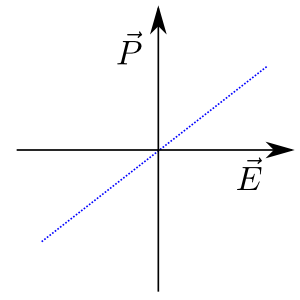
\includegraphics[width=0.9\linewidth]{./figs/chap1/dielpolplot}
	\caption{Dielectric}
	\label{fig:dielplot}
\end{subfigure}
\begin{subfigure}{0.3\textwidth}
\centering
	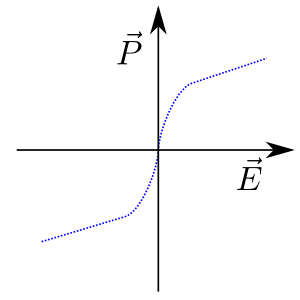
\includegraphics[width=0.9\linewidth]{./figs/chap1/parelpolplot}
	\caption{Paraelectric}
	\label{fig:parelplot}
\end{subfigure}
\begin{subfigure}{0.3\textwidth}
\centering
	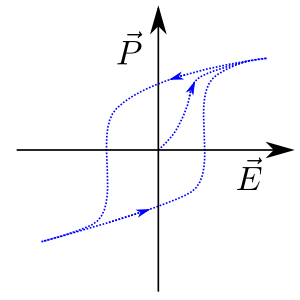
\includegraphics[width=0.9\linewidth]{./figs/chap1/ferelpolplot}
	\caption{Ferroelectric}
	\label{fig:ferelplot}
\end{subfigure}
\caption{Schematic polarisation plots for different types of materials.}
\label{fig:polplot}
\end{figure}
In Figure \ref{fig:polplot} three polarisation plots, $\vec{P}$ vs. $\vec{E}$, for three different classes of materials are shown. Figure \ref{fig:dielplot} shows the behaviour of a \enhyphen{normal}~\footnote{\ie{} linear, homogeneous, isotropic} dielectric material. The slope of the polarisation curve corresponds to the material's electric permittivity $\epsilon$ and is a constant. Figure \ref{fig:parelplot} depicts the behaviour of a paraelectric material. The \enhyphen{kink} in the curve is explained by the material becoming inherently polarised at an applied electric field: once a certain threshold applied magnetic field is reached, all previously unaligned dipoles in the material are aligned against the applied field and weaken it to the maximum extend possible for that material. When the external field is removed, the dipoles return to their unaligned state and the material thus loses its polarisation. Lastly, Figure \ref{fig:ferelplot} depicts the polarisation plot of a ferroelectric material. These materials exhibit a spontaneous electric polarisation that can be reversed by an applied field, leading to a hysteretic loop in the polarisation plot. As the applied field strength increases, so does the material's polarisation up to a point where all dipoles are aligned against the applied field. This alignment is retained in the material, leading to a non-zero polarisation at zero applied electric field. When the field is applied in the reverse direction and reaches a sufficient strength, the ordering in the material reverses as well, leading to symmetry around the axes observed in the polarisation plot.\\
\begin{figure}
\begin{subfigure}{0.3\textwidth}
\centering
	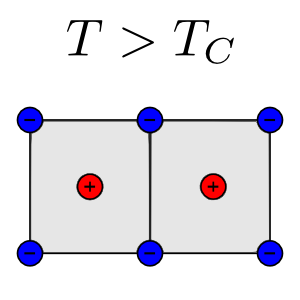
\includegraphics[width=0.9\linewidth]{./figs/chap1/ferroscheme1}
	\caption{}
	\label{fig:ferroscheme1}
\end{subfigure}
\begin{subfigure}{0.3\textwidth}
\centering
	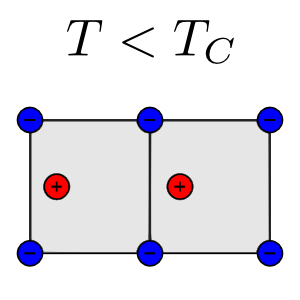
\includegraphics[width=0.9\linewidth]{./figs/chap1/ferroscheme2}
	\caption{}
	\label{fig:ferroscheme2}
\end{subfigure}
\begin{subfigure}{0.3\textwidth}
\centering
	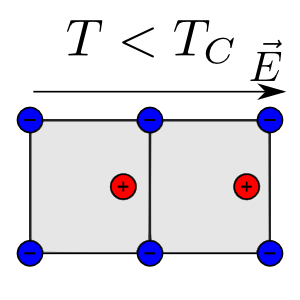
\includegraphics[width=0.9\linewidth]{./figs/chap1/ferroscheme3}
	\caption{}
	\label{fig:ferroscheme3}
\end{subfigure}
\caption[Schematic representation of the structural phases in a ferroelectric at a temperature above the Curie temperature (\ref{fig:ferroscheme1}), below the Curie temperature (\ref{fig:ferroscheme2}) and below the Curie temperature in the presence of an external electric field (\ref{fig:ferroscheme3}).]{Schematic representation of the structural phases in a ferroelectric at a temperature above the Curie temperature (\ref{fig:ferroscheme1}), below the Curie temperature (\ref{fig:ferroscheme2}) and below the Curie temperature in the presence of an external electric field (\ref{fig:ferroscheme3}). Adopted from Kittel~\cite[p. 478]{kittel}.}
\label{fig:ferroscheme}
\end{figure}
It is usual for a ferroelectric material to lose its ferroelectricity above a material specific Curie temperature $T_C$, \ie{} most ferroelectric materials undergo a ferroelectric/paraelectric phase transition at $T_C$ because the internal dipoles are coupled to the material lattice. Temperature naturally influences the lattice and therefore, the dipoles, see Figure \ref{fig:ferroscheme} for an overview of the structural phases at different temperatures. Ferroelectric transitions are broadly classified into two main groups at the extremes of a continuous spectrum: order-disorder and displacive transitions~\cite[pp. 467 ff.]{kittel}. Order-disorder transitions are relatively simply characterised by the fact that the  in the unit cells point in random directions above $T_C$. In a displacive transition, the polarisation of the material becomes unusually large, leading to a \enhyphen{polarisation catastrophe}: the local electric field caused by a displacement of charge is stronger than the elastic restoring force, leading to an asymmetrical shift of charges. In close analogy with ferromagnetism, ferroelectric domains may exist in a ferroelectic material. Each domain is characterised by a polarisation in the same direction, whereas adjacent domains have a polarisation in a different direction. The net polarisation of the material is the vector-sum of the contributions of the individual domain polarisations and the total polarisation of the material can be changed by movement of domain walls or by nucleation of new domains.
\newpage
\section{Polyvinylidene Difluorite and its Copolymers}
\begin{figure}[h]
\centering
	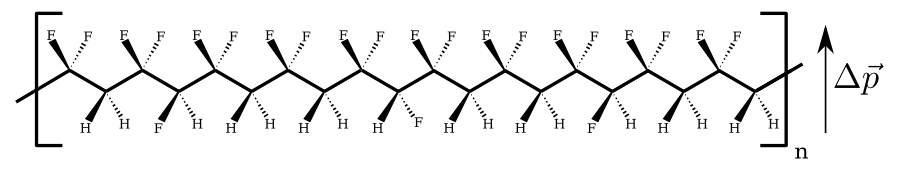
\includegraphics[width=0.9\textwidth]{./figs/chap1/pvdfstruct}
	\caption{An approximate chemical structure for \pvtr{}. The direction of the dipole moment, from Hydrogen to Fluorine, is indicated.}
	\label{fig:pvstruct}
\end{figure}
Polyvinylidene difluorite (\pvdf{}) is a ferroelectric polymer that is used on an industrial scale as a speciality plastic. On the industrial level, it is largely more interesting because its chemical properties than its ferroelectricity: its melting point, $\sim$\SI{177}{\degreeCelsius}, is relatively low compared to other fluoropolymers and is therefore more easily processed, yet it retains the stability with respect to acids, bases, solvents and heats typical for the fluorofamily. It is an insulator with a relatively low density, $\sim$\SI{1.8}{\gram\per\cubic\centi\metre}, and high mechanical strength. It is therefore often used for piping, wire-insulation, tubing etc. With regards to its ferroelectric behaviour \pvdf{} is often employed as a copolymer which includes trifluoroethylene (\trfe{}) in its chains. These copolymers are collectively referred to as \pvfe{} usually identified by the molar ratio of their constituent difluoro- and trifluoroethylene groups. For this project \pvtr{} was available and except where otherwise specifically noted, the terms \pvdf{} and \pvtr{} may be used synonymously. An approximate chemical structure for \pvtr{} is depicted in Figure \ref{fig:pvstruct}. The structure is only approximate because the exact position of \trfe{} in the chain is random, but will on average approach a distribution that reflects the molar ratio.\\
The \emph{\enhyphen{Encyclopedia of Smart Materials}} devotes an entire Chapter to polyvinylidene difluorite and its copolymers~\cite[pp. 807-820]{encyclopedia} and much of the following discussion is largely based on this excellent summary.\\
\begin{figure}
\begin{subfigure}{0.5\textwidth}
\centering
	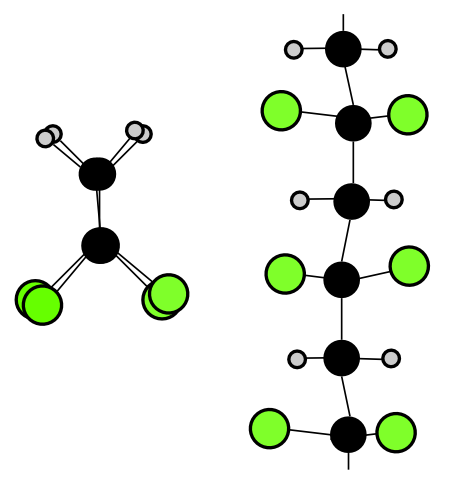
\includegraphics[width=0.8\linewidth]{./figs/chap1/pvdfbeta}
	\caption{All-\emph{trans} $\beta$-phase, designated TTT}
	\label{fig:pvdfbeta}
\end{subfigure}
\begin{subfigure}{0.5\textwidth}
\centering
	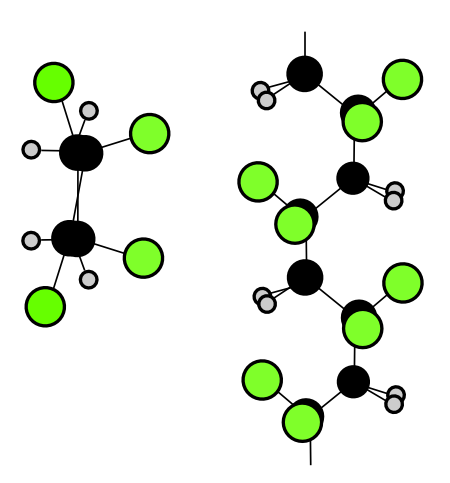
\includegraphics[width=0.8\linewidth]{./figs/chap1/pvdfalpha}
	\caption{$\alpha$-phase, designated TGT$\bar{\text{G}}$}
	\label{fig:pvdfalpha}
\end{subfigure}
\caption[Along-the-chain and top down views of ball and stick models for two crystalline forms of pure \pvdf{}. Fluorine atoms are green, carbon black, hydrogen grey.]{Along-the-chain and top down views of ball and stick models for two crystalline forms of pure \pvdf{}. Fluorine atoms are green, carbon black, hydrogen grey. Adopted from~\cite[p. 809]{encyclopedia}.}
\label{fig:pvdfstruct}
\end{figure}
\begin{figure}
\centering
	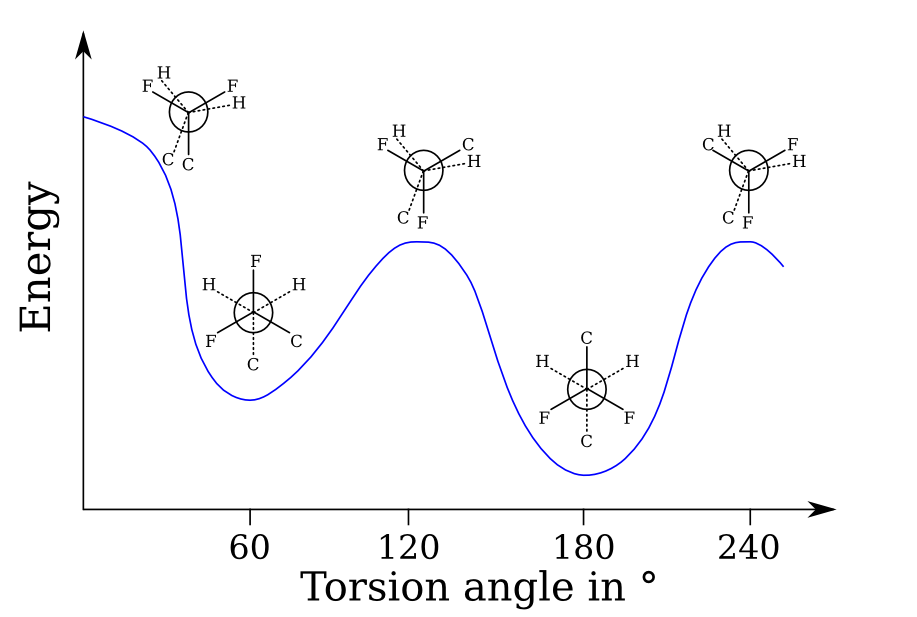
\includegraphics[width=0.9\textwidth]{./figs/chap1/fischerproject}
	\caption[Fischer-Projections and internal energy as a function of the torsion angle along the chain. The minimum at \ang{180} corresponds to the \emph{trans} $\beta$-phase.]{Fischer-Projections and internal energy as a function of the torsion angle along the chain. The minimum at \ang{180} corresponds to the \emph{trans} $\beta$-phase. Adopted from~\cite[p. 809]{encyclopedia}.}
	\label{fig:pvfischer}
\end{figure}
Overall, the structure of the (co)polymer is semi-crystalline and will consist of ordered regions of monomer units, crystallites of $\sim$\SIrange{10}{20}{\nano\metre} surrounded by a sea of amorphous, scrambled chains. The polymer may furthermore include regions of head-to-tail bonding (--CH$_2$--CF$_2$--CH$_2$--CF$_2$--) alongside regions of tail-to-tail and/or head-to-head bonding (--CH$_2$--CF$_2$--CF$_2$--CH$_2$-- and --CF$_2$--CH$_2$--CH$_2$--CF$_2$-- respectively) which can be categorised as defects in the crystalline regions of \pvdf{}. In the case of the copolymer, \trfe{} is incorporated atacticly into the molecule, \ie{} the position of the third vinyl-group with respect to the chain~\footnote{Either \enhyphen{in front of} or \enhyphen{behind} the chain} is random. Disregarding these defects, there are four major crystalline forms of \pvdf{} which are described by the way the chains are packed within the crystal lattice: according to their conformations (\emph{trans} (T) or \emph{gauche} (G) linkages), their orientation about the chain axis (\emph{parallel} or \emph{antiparallel}) and the relative directions of adjacent chains (\emph{up-up} when pointing in the same and \emph{down-down} when pointing in opposite directions). Figure \ref{fig:pvdfstruct} depicts two of the the major crystalline forms and it is apparent from the Fischer-projections in Figure~\ref{fig:pvfischer} that the all-\emph{trans} $\beta$-phase will be preferred, resulting in a dipole-moment of $\sim$\SI{2.1}{D}~\footnote{The debye is a CGS-unit convenient for molecular dipole-moments. It is exactly equivalent to \SI{1e-21}{\coulomb\metre} divided by the speed of light and  approximately equal to \SI{0.2082}{\elementarycharge\angstrom}.} in pure \pvdf{}~\cite[p. 810]{encyclopedia}. Figure \ref{fig:pvdfunit} compares the orthorhombic unit cells of the $\beta$- and $\alpha$-phases of \pvdf{} and shows an absence of a permanent dipole in the latter. The polymer chain lies along the $\vec{c}$ unit cell vector. Table \ref{tab:pvdflat} summarises the lattice dimensions and angles of pure \pvdf{} in the the $\alpha$- and $\beta$-phase and includes lattice parameters for the $\beta$-phase of \pvfe{} of varying molar ratio. It is apparent that introducing a third Fluorine atom into the unit cell will reduce the net dipolar moment of the monomer unit, but because of atacticity, the net dipole-moment is still parallel to the $\vec{b}$ unit cell vector. The macroscopic effect on the net polarisation may not be as easily inferred because inclusion of \trfe{} may influence the superstructure of the polymer, the ordering of its crystallites and possibly the structure of its ferroelectric domains. The ferroelectric/paraelectric phase transition in \pvdf{} is an order-disorder transition of first order~\cite{takeo}. The $\delta$-phase will not be discussed here.
\begin{figure}
\begin{subfigure}{0.5\textwidth}
\centering
	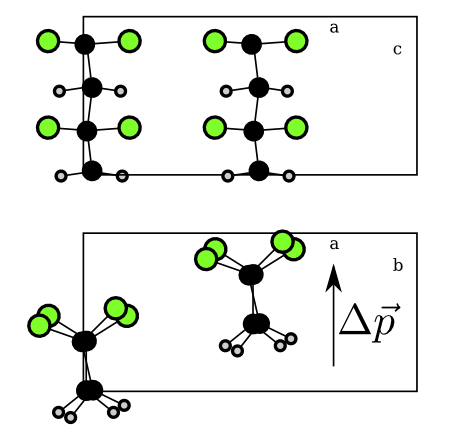
\includegraphics[width=0.8\linewidth]{./figs/chap1/betaunitcell}
	\caption{$\beta$-phase}
	\label{fig:betaunitcell}
\end{subfigure}
\begin{subfigure}{0.5\textwidth}
\centering
	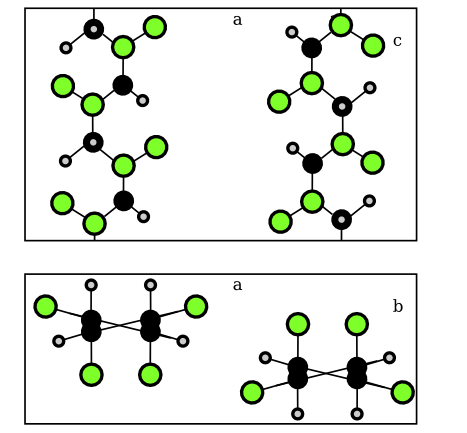
\includegraphics[width=0.8\linewidth]{./figs/chap1/alphaunitcell}
	\caption{$\alpha$-phase}
	\label{fig:alphaunitcell}
\end{subfigure}
\caption[Schematic representations of the unit cells of two crystalline phases of \pvdf{}. Fluorine atoms are green, carbon black, hydrogen grey. The direction of the dipole moment in the $\beta$-phase is indicated.]{Schematic representations of the unit cells of two crystalline phases of \pvdf{}. Fluorine atoms are green, carbon black, hydrogen grey. The direction of the dipole moment in the $\beta$-phase is indicated. Adopted from~\cite[pp. 809 f.]{encyclopedia}.}
\label{fig:pvdfunit}
\end{figure}
\begin{table}
\centering
\caption[Experimental Lattice Dimensions and Angles of pure \pvdf{} ($\alpha$ and $\beta$) and of \pvfe{} ($\beta$) of varying molar ratio.]{Experimental Lattice Dimensions and Angles of pure \pvdf{} ($\alpha$ and $\beta$) and of \pvfe{} ($\beta$) of varying molar ratio. Compiled from~\cite[p. 810]{encyclopedia}.}
\label{tab:pvdflat}
\begin{tabular}{@{}l l l l l l l l@{}}
\toprule
\multirow{2}{*}{\parbox[c]{2.5cm}{\trfe{} content in \si{\mole\percent}}} & \multirow{2}{*}{\parbox[c]{2.5cm}{Crystalline Phase}} & \multicolumn{3}{l}{Lattice Dimensions (\si{\angstrom})} & \multicolumn{3}{l}{Lattice Angles (\si{\degree})} \\ \cmidrule(l){3-8} 
                                                       &                                    & a                 & b                 & c                & $\alpha$        & $\beta$        & $\gamma$       \\ \midrule
0                                                      & $\alpha$                           & 4.69              & 9.64              & 4.62             & 90              & 90             & 90             \\
0                                                      & $\beta$                            & 8.58              & 4.91              & 2.56             & 90              & 90             & 90             \\
25                                                     & $\beta$                            & 8.86              & 4.62              & 2.56             & 90              & 90             & 90             \\
50                                                     & $\beta$                            & 9.12              & 5.25              & 2.56             & 90.3            & --             & --             \\ \bottomrule
\end{tabular}
\end{table}
Because of unfavourable, repulsive van der Waals interactions introduced by the third Fluorine, the melting point of the copolymer decreases with increasing \trfe{} content and for the same reason, incorporating \trfe{} furthermore favours crystallisation into the $\beta$-phase. It can be seen in Figure \ref{fig:pvdfunit} that the Fluorines in the $\alpha$ unit cell are more closely packed. Therefore, melting temperature $T_m$, phase transition temperature $T_C$, degree of crystallinity, remnant polarisation $P_r$ and coercive field $E_C$ are all affected by the \trfe{} content, which is summarised in Table \ref{tab:trfecont}. However, even if the polymer is present in the ferroelectric phase, its ferroelectric domains will non the less be oriented in all crystallographically allowed directions. For an observable net polarisation to develop, the polymer therefore has to be \enhyphen{poled}: in a strong electric field, dipolar ordering will be added to crystalline ordering. Elevated annealing temperatures will help with this process even if $T_C$ is exceeded, because as the polymer cools down, the preferred ferroelectric phase will crystallise with a higher degree of oriented ferroelectric domains. The effect of annealing temperature on crystallinity and remnant polarisation for a \pvfe{} with \SI{32}{\mole\percent} \trfe{} is shown in Figure \ref{fig:annealtemp}. Poling is usually accomplished either by electroding the polymer surfaces or by the use of a corona discharge where charge is injected into the polymer. For this project, electrode poling, both contacted and non-contacted, was attempted. Lastly, it was reported that \pvdf{} thin films obtained from Langmuir-Blodgett (\lb{}) deposition crystallise directly in the $\beta$-phase and undergo self-polarisation~\cite{chen_lbpvdf,kliem_lbpvdf}. However, \lb{} deposition was not easily available during the course of this project and this route could therefore not be explored.
\begin{table}
\centering
\caption[Degree of crystallinity, melting temperature $T_m$, phase transition temperature $T_C$, remnant polarisation $P_r$ and coercive field $E_C$ for \pvfe{} copolymers of varying molar ratio.]{Degree of crystallinity, melting temperature $T_m$, phase transition temperature $T_C$, remnant polarisation $P_r$ and coercive field $E_C$ for \pvfe{} copolymers of varying molar ratio. Some values are approximations because data was visually compiled from figures~\cite[pp. 812 f.]{encyclopedia}.}
\label{tab:trfecont}
\begin{tabular}{@{}llllll@{}}
\toprule
\parbox[c]{2.5cm}{\trfe{} content in \si{\mole\percent}} & Crystallinity (\si{\percent}) & $T_m$ (\si{\degreeCelsius}) & $T_C$ (\si{\degreeCelsius}) & $P_r$ (\si{\milli\coulomb\per\square\metre}) & $E_C$ (\si{\mega\volt\per\metre}) \\ \midrule
0 	& 50 		  & \phantom{$\sim$}178 		& $\sim$195 				& \phantom{$\sim$}50 	& \phantom{$\sim$}50 	\\
22 	& \num{80+-4} & \phantom{$\sim$}150 		& \phantom{$\sim$}140 	& $\sim$63 				& \phantom{$\sim$}65 	\\
26 	& \num{84+-4} & \phantom{$\sim$}150 		& \phantom{$\sim$}130 	& \phantom{$\sim$}75		& $\sim$69 				\\
31 	& \num{88+-4} & \phantom{$\sim$}145 		& \phantom{$\sim$}110 	& $\sim$83 				& \phantom{$\sim$}70 	\\
36 	& \num{91+-4} & \phantom{$\sim$}160 		& \phantom{$\sim$}94  	& $\sim$93 				& \phantom{$\sim$}75 	\\
50 	& \num{73+-4} & $\sim$163 				& \phantom{$\sim$}55	 	& \phantom{$\sim$}63		& \phantom{$\sim$}45 	\\ \bottomrule
\end{tabular}
\end{table}
\begin{figure}[h]
\centering
	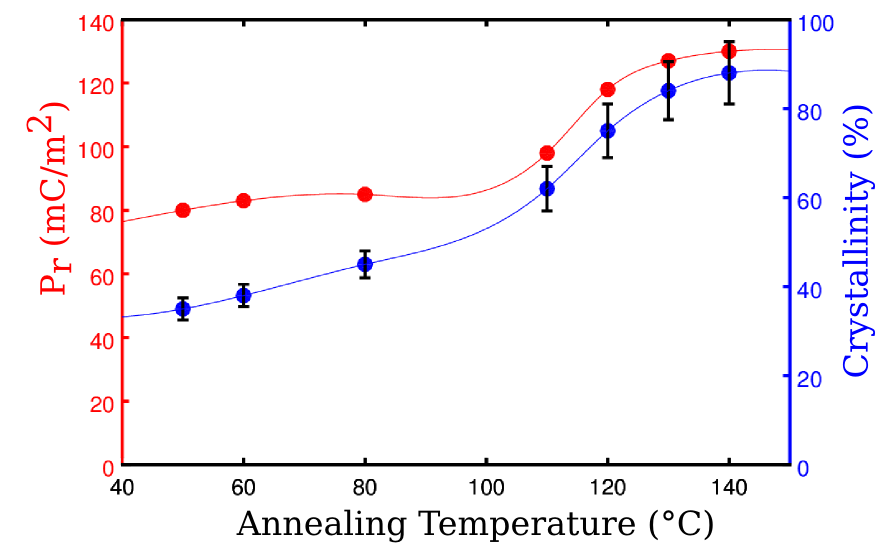
\includegraphics[width=0.9\textwidth]{./figs/chap1/annealtemp}
	\caption[Effect of annealing temperature on remnant polarisation $P_r$ and degree of crystallinity in \pvfe{} with a \trfe{} content of \SI{32}{\mole\percent}.]{Effect of annealing temperature on remnant polarisation $P_r$ and degree of crystallinity in \pvfe{} with a \trfe{} content of \SI{32}{\mole\percent}, adopted from~\cite[p. 813]{encyclopedia}. The line through the data points was constructed with a spline fit and is not based on a physical model.}
	\label{fig:annealtemp}
\end{figure}
\subsection{\pvdf{} Nanoparticles}
Apart from bulk material and thin films, \pvdf{} can also be prepared as nanoparticles (\nps{}) and as nanostructured material. While interesting, \pvdf{} nanostructures require sophisticated preparation steps, whereas \pvdf{} \nps{} can easily be synthesised by a scalable, solution chemistry self-assembly mechanism which sidesteps the otherwise necessary high annealing temperatures, rendering this route especially interesting for the application with organic photovoltaic cells (\opvs{}). The reproducible synthesis was first described by Xiao~\etal{}~\cite{NPsynthesis} and their paper serves as a basis for the following discussion of the properties of \pvdf{} \nps{}. To achieve self-assembly of \pvdf{}-chains into nanoparticles, the polymer is first dissolved in a \enhyphen{good} solvent, such as acetone, and then an interface with a \enhyphen{bad} solvent, such as water, is formed. At the interface, \pvdf{} chains tend to coils in on themselves because of the strong hydrophobic interaction between water and fluorine in \pvdf{}. This process is supported by precipitating the \nps{} out with the help of a high speed centrifuge at speeds around \SI{20000}{rpm}. Because water cannot form hydrogen bonds with the polymer~\cite{silverstein}, an increase in entropy results, causing subsequent polymer chains to aggregate at the surface of the forming \np{}. The \nps{} crystallise in \pvdf{}'s amorphous, non-ferroelectric phase but can be converted to the crystalline, ferroelectrically  active $\beta$-phase by heating above its Curie temperature. This is achieved by refluxing the suspension of \nps{}, which can subsequently be processed further. Spin-coating, evaporating or simply mixing the suspension with other chemicals allow for the \nps{} to be included in \opvs{} in a non-destructive, controlled manner: for example, Xiao~\etal{} could independently optimise the nanoparticle size and their coverage in the solar cell. \pvdf{} is a non-conducting polymer and as such increases the series resistance of the solar cell, counteracting its positive influences on charge carrier recombination lifetimes. For the optimised coverage of \SI{18}{\percent}, the solar cell's efficiency could be improved by \SI{1.9}{\percent} from \SI{4.74}{\percent} to \SI{6.64}{\percent} which is a sizeable relative improvement of $\sim$\SI{29}{\percent}!

\section{Experimental Techniques}
\label{sec:exptech}
\subsection{Contact Potential Difference and Surface Photovoltage}
Chapter \ref{chap:spv} deals exclusively with the contact potential difference (\cpd{}) and the surface photovoltage (\spv{}), so any theoretical or practical explanation will be skipped here.\\
For the scope of this Chapter, it is sufficient to mention that \cpd{} measures the work function of a sample compared to a known reference and that \spv{} can be an indicator of charges trapped at the surface and the overall quality of a chemical or physical surface modification. Previous work carried out at the Cahen group often focused on chemical surface modifications of silicon and it was shown for a range of chemicals that a (surface) dipole can influence the work function of the underlying silicon substrate. It is therefore assumed that successfully adsorbed \pvdf{} should influence the work function of silicon as measured by \cpd{} and that the direction of this influence be tune-able by changing the polarisation-direction of the ferroelectric polymer. It is furthermore assumed that a change in \spv{} may be taken as an indication of either less surface recombination or the presence of an electrical field at the surface.

\subsection{Determination of Excess Carrier Lifetimes}
In semiconductors, photogenerated excess charge carriers may recombine via different mechanisms. The effects of each of these mechanisms can be described by individual recombination rates, $S$ or by individual characteristic recombination \enhyphen{lifetimes}, $\tau$. Generally, a distinction has to be made between recombination in the bulk as expressed by the bulk carrier lifetime \tbulk{} and recombination at surfaces as expressed by the surface lifetime \tsurf{}. These two lifetimes combine to an effective carrier lifetime \teff{} given by:
\begin{equation}
\label{efflifetime}
	\frac{1}{\teff} = \frac{1}{\tbulk} + \frac{1}{\tsurf} \, .
\end{equation}
For the bulk, three mechanism can be identified: radiative recombination (also known as band-to-band recombination), \trad{}, where carriers of opposite charge neutralise each other and emit a photon of corresponding energy; Shockley-Read-Hall recombination , \tsrh{}, where carriers recombine via traps within the bandgap and Auger recombination, \taug{}, where opposite carriers recombine and transfer their energy to a third carrier, which subsequently gives off its excess energy in the form of heat. In the presence of these mechanisms, \tbulk{}, is given by:
\begin{equation}
\label{bulklifetime}
	\frac{1}{\tbulk} = \frac{1}{\trad} + \frac{1}{\tsrh} + \frac{1}{\taug} \, .
\end{equation}
For indirect bandgap semiconductors such as silicon, \trad{} is typically large compared to the other times and may be neglected in Equation \eqref{bulklifetime}. Conversely, for (high quality) direct bandgap semiconductors such as GaAs, \trad{} is short and \tsrh{} is typically large and may often be neglected~\cite{gaaslifetime}. Because Auger recombination is a three-particle process, it is inherently less probable than its two-particle counterparts. However, the Auger recombination rate is a cubic function of excess carrier density and therefore becomes dominant at higher carrier concentrations~\cite{auger}. Surfaces are natural defects in the crystal structure and as such provide ample opportunity for carriers to recombine. It is more difficult to generally relate the surface recombination velocities \ssurf{} to a surface recombination lifetime which can be used in Equation \eqref{efflifetime}. For example, the two large surfaces of a wafer might have different recombination velocities and in very high quality semiconductors, even the comparatively small surfaces at the edges may influence the overall effective lifetime~\cite{edgerecom}.\\
One method to measure the effective lifetime of the excess carriers of a semiconductor is to convert its photoconductance into its excess carrier density via known mobility functions:
\begin{equation}
\label{carrierbalance}
	\Delta n = \frac{\Delta \sigma}{qW (\mu_n \mu_p)} \, ,
\end{equation}
where $\sigma$ is the conductance, $\Delta n$ denotes the excess carrier density, $W$ is the sample thickness, $q$ the charge and $\mu_n$ \& $\mu_p$ are the mobilities of negative and positive carriers respectively. The situation is complicated because the mobilities generally are functions of the doping densities and also of the excess carrier density~\cite{sintononline}. Therefore, some knowledge about the sample is required and modelling the characteristics of the sample is generally applied. The carrier concentration in Equation \eqref{carrierbalance} can be converted to lifetimes by solving the continuity equations to obtain:
\begin{equation}
\label{taugeneral}
	\teff (\Delta n) = \frac{\Delta n (t)}{G(t) - \frac{d\Delta n}{dt} } \, ,
\end{equation}
in which $G(t)$ is the photogeneration rate and $\Delta n$ is, again, the excess carrier density~\cite{nagel_lifetime}. Equation \eqref{taugeneral} is generally valid and was even derived for non-uniform photogeneration in the presence of significant surface recombination. Most measurements are realised by flashing a strong light on the sample and monitoring the time-evolution of its photoconductance via a radio-frequency bridge. When the duration of the flash is long, a quasi-steady state situation is achieved in which the excess carrier density can be seen as constant in time. Equation \eqref{taugeneral} simplifies to:
\begin{equation}
\label{qsspd}
	\teff (\Delta n) = \frac{\Delta n (t)}{G(t)} \, ,
\end{equation}
which is a good approximation for short lifetimes. A drawback of this method is that the generation rate must be known. Therefore the intensity of the flash has to be monitored, corrected for reflectivity and absorption by the sample. The opposite situation, a transient photoconductance decay measurement, is achieved then the flash is very brief and no illumination reaches the sample during the measurement. Then, the photogeneration rate can be assumed to be zero and Equation \eqref{taugeneral} can be solved to obtain:
\begin{equation}
\label{tpd}
	\teff (\Delta n) = - \frac{t}{\ln (\Delta n)} \, .
\end{equation}
This approach is only valid for relatively long lifetimes, but the intensity of the flash does not need not be monitored and reflectivity \& absorption of the sample do not need to be known, either. The combined quasi-steady-state, quasi-transient approach as described by Equation \eqref{taugeneral} yields the most accurate results, but is also the most involved. For this approach to work, the intensity of the flash must be measured in real-time and the absolute conductance of the sample must be known, as described by Sinton \emph{et~al.}~\cite{sinton1,sinton2}.\\
In all cases, if one is interested in the surface recombination velocities or lifetimes, \teff{} needs to be translated into \tbulk{}. Experimentally, this can most easily be achieved by using a high quality substrate in which $\tbulk \gg \teff$. If the latter is not the case, then there is an exact equation that can be used for transient measurements:
\begin{equation}
\label{exacttransient}
	\ssurf = \sqrt{D \left( \frac{1}{\teff} - \frac{1}{\tbulk} \right)} \tan \left( \frac{W}{2} \sqrt{D \left( \frac{1}{\teff} - \frac{1}{\tbulk} \right)} \right) \, ,
\end{equation}
where $D$ is the minority carrier diffusivity and the other symbols have their usual meaning~\cite{luke_lifetime}. A series of approximations to that equation exists and they are valid if $\teff \gg \frac{W^2}{\pi ^2 D}$ for transient measurements and if $\teff \gg \frac{W^2}{12 D}$ for quasi-steady state measurements~\cite{sproul_lifetime}. 

\subsection{Infrared Spectroscopy}
\sisetup{per-mode = reciprocal-positive-first}
Infrared (\ir{}) spectroscopy is a vibrational spectroscopy which employs light with energies just below the visible spectrum, \ie{} with wavelengths longer than $\sim$ 800 nm. It is common to express the spectrum in terms of its frequency and a typical unit is reciprocal centimeters (\si{\per\centi\metre}), also called \enhyphen{wavenumbers} and to divide it into three broad regions: \enhyphen{near \ir{}} ($\sim$ \SIrange{14e3}{4e3}{\per\centi\metre}), \enhyphen{mid \ir{}} ($\sim$ \SIrange{4e3}{0.4e3}{\per\centi\metre}) and \enhyphen{far \ir{}} ($\sim$ \SIrange{400}{10}{\per\centi\metre}), where each region approximately excites different types of vibrations ranging from harmonic to rotational-vibrational excitations. Vibrational modes are \ir{}-active if there is a change in dipole moment which enables interaction with the electric field of the radiation. Therefore \ir{} spectroscopy is very sensitive to the chemical environment of the sample under investigation and is especially frequently used in organic chemistry. Practically, instead of scanning each wavenumber individually, the sample is often illuminated by a wide range of radiation and decomposed by a Fourier transformation into its components, yielding Fourier Transform \ir{} (\ftir{}) spectroscopy which shortens the time of the measurement and allows detecting small quantities of and minute changes in a sample.\\%
\sisetup{per-mode = symbol}%
\begin{figure}
\begin{subfigure}{0.5\textwidth}
\centering
	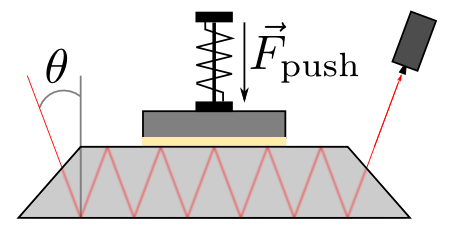
\includegraphics[width=0.8\linewidth]{./figs/chap1/IRoverview}
	\caption{}
	\label{fig:iroverview}
\end{subfigure}
\begin{subfigure}{0.5\textwidth}
\centering
	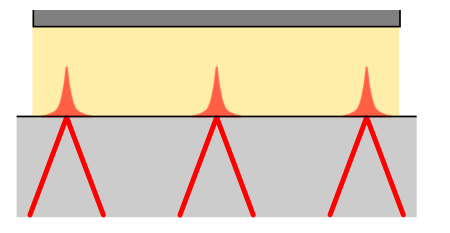
\includegraphics[width=0.8\linewidth]{./figs/chap1/IRwave}
	\caption{}
	\label{fig:irwave}
\end{subfigure}
\caption[Schematic of an \atr{} \ftir{} set-up. Figure \ref{fig:iroverview} shows the internal reflection of the beam of light at the edges of the guiding crystal (light gray) and the thin film sample (yellow) on its substrate (dark grey) being pressed onto the crystal. Figure \ref{fig:irwave} focuses on the evanescent wave projecting into the thin film and gives an indication how the beam, while being nominally inside the crystal, can still be attenuated by the sample.]{Schematic of an \atr{} \ftir{} set-up. Figure \ref{fig:iroverview} shows the internal reflection of the beam of light at the edges of the guiding crystal (light gray) and the thin film sample (yellow) on its substrate (dark grey) being pressed onto the crystal. Figure \ref{fig:irwave} focuses on the evanescent wave projecting into the thin film and gives an indication how the beam, while being nominally inside the crystal, can still be attenuated by the sample. Adopted from VILAN.}
\label{fig:irscheme}
\end{figure}
To study thin films that are either physically or chemically adsorbed to a substrate surface, it is useful exclude interaction of the substrate with the \ir{}-radiation and to maximise the interactions interactions that are of interest. One method that accomplishes  both these goals is Attenuated Total Reflectance (\atr{}) \ftir{} where the \ir{} beam is directed into a crystal of high refractive index and reflects internally from its surfaces. Refer to Figure \ref{fig:irscheme} for a schematic of the \atr{} method. The thin film under investigation is pressed onto the crystal to form an intimate contact so that an evanescent \ir{} wave can project into it, see Figure \ref{fig:irwave}. There, part of the \ir{} spectrum is absorbed by the sample and the now somewhat reduces beam is returned into the crystal where it can be internally reflected to be projected into the thin film again multiple times, greatly attenuating the absorption of the thin film. As can be deduced from Figure \ref{fig:iroverview}, the reflectance is given by
\begin{equation}
\label{atr-reflectance}
	R(\lambda)^N = (1-a_{\lambda} \cdot d_e)^N \, ,
\end{equation}
where $N$ is the number of reflections taking place at the crystal/thin film interface~\footnote{For the case of Figure \ref{fig:irscheme} $N=3$}, $a_{\lambda}$ is the wavelength specific absorptivity of the thin film and $d_e$ is its effective thickness. One complication that needs to be mentioned is that \atr{} spectra are not linear with wavenumber CITE VILAN and therefore sometimes difficult to compare to transmittance spectra. In the context of this study, that complication is somewhat alleviated because we will mainly compare \atr{}-\ftir{} spectra relative to other other \atr{}-\ftir{} spectra to assess whether or not a phase transition has occurred in the thin film sample and will for the most part not need absolute quantification of the samples.
\subsection{Ellipsometry and Contact Profilometry}
\subsubsection{Ellipsometry}
Generally, ellipsometry is an optical technique for investigating the dielectric properties of (layers of) thin films of material(s) on reflective surfaces. It is an indirect method insofar as that the information obtained from an ellipsometry measurement cannot directly be converted into the dielectric properties of the thin film under investigation. Therefore, the measured data must be compared to a model and the success of an ellipsometry measurement hinges on the quality of that model. In its most common form, ellipsometry measures the properties of light reflected from the surface of a sample. The set-up consists of a light source, a polariser, the sample, an analyser and a detector. Light with known, elliptical polarisation is employed, hence the name. This incident light can be decomposed into two components: the \emph{s} component where the electrical field of the radiation oscillates parallel to the sample and perpendicular to the plane of incidence and the \emph{p} component where the field oscillates parallel to the plane of incidence. Ellipsometry measures the complex reflectance $\rho$ of the sample which consists of an amplitude component $\Psi$ and a phase difference $\Delta$ according to
\begin{equation}
	\rho = \tan \left( \Psi \right) \exp \left( i \Delta \right) \, .
\end{equation}
The complex nature of the reflectance as measured by ellipsometry is readily apparent from the equation above. Per wavelength, one pair of $\Psi$ \& $\Delta$ can be obtained. Therefore, to reach more optical parameters, a broad spectrum is often employed in ellipsometry. For the purposes of this study, ellipsometry was exclusively used to find the thickness of a layer of interest on a substrate of known composition and thickness.
\subsubsection{Contact Profilometry}
Contact profilometry is a conceptually exceedingly simple technique to study surfaces and their roughness. A small diamond tip is brought in contact with a surface and moved across a predefined path along that surface and vertical displacement of the stylus is measured accurately. Depending of the type of surface under investigation displacements of \SI{10}{\nano\metre} up to \SI{1}{\micro\metre} can typically be measured with a lateral resolution depending primarily on the size of the tip-apex, where resolutions of $\sim$\SI{20}{\nano\metre} are feasible. The diamond tip of a record player scanning a vinyl record and producing an audible, analogue signal is a very fitting analogy for contact profilometers in use today.
\subsection{Electron Microscopy}
While a thorough explanation of the function and uses of electron microscopy is out of the scope of this paper, a brief introduction to Scanning Electron Microscopy (\sem{}) for the visualisation of nanometre sized objects will still be given. \sem{} is a type of electron microscopy in which a sample is raster-scanned with a focused beam of electrons. This focused beam causes the sample to emit several types of signals: secondary electrons emitted by atoms in the sample, backscattered electrons, x-rays and light of varying wavelength and intensity, all of which can be detected by sophisticated microscopes. The resolution of the microscope is not achieved as in an optical microscope or as in a Transmission Electron Microscope (\tem{}) where the focusing the beam and the wavelength are determining, but rather by a translation of the size of the raster on the sample to the size of the raster on the detector. Thus, \sem{} can cover up to six orders of magnitude of magnification and sample features at very different length scales can be investigated. Because the sample is subjected to a continuous beam of electrons, it needs to be conductive and grounded to get rid off excess charge. Charge accumulated on the sample can lead to unwanted interactions and artefacts in the visual reconstruction of the sample. For the purpose of this study, \sem{} was used to investigate the surface morphology of deposited thin films of a polymer, \pvdf{}, and nanoparticles synthesised from the same polymer. \sem{} was also used to obtain typical nanoparticle dimensions.
\subsection{IV-Curves}
Current-Voltage curves (IV-curves) of a semiconductor or solar cell can reveal a lot of information about the semiconductor or cell under investigation, not withstanding its conceptual simplicity. In a straight forward measurement, two contact are electrically connected to the sample and the current resulting from a precisely known applied voltage is measured accurately. With an appropriate illumination set-up, dark and light IV-curves can be obtained and compared. For an ideal diode, the dark current is given by the diode equation:
\begin{equation}
	I = I_0 \left( \exp \left( \frac{qV}{nk_BT} \right) -1 \right) \, ,
\end{equation}
where $I_0$ is the reverse saturation bias current, $n$ is the ideality factor and the remaining symbols have their usual meaning. Under light conditions, a steady-state current is induced that shifts the IV-curve down, depending on the size of the photon-current, their spectrum and the cell's spectral response. A \enhyphen{real} diode will also include parasitic resistances such as series resistance $R_S$ and shunt resistance $R_{SH}$ and the measured IV-curve will more closely follow a form corresponding to the equation:
\begin{equation}
	I = I_0 \left( \exp \left( \frac{q(V+IR_S)}{nk_BT} \right) -\frac{V+IR_S}{R_{SH}} \right) \, .
\end{equation}
As can be seen from the above equation, the parasitic resistances can be obtained from the derivative of of the IV-curve at its intersections with the axes and to put it more colloquially, parasitic resistances will result in the IV-curve being \enhyphen{less square} than than of its ideal counterpart. The presence of back-diodes will result in a \emph{S}-shaped or otherwise generally misshapen IV-curves and while it is often useful to extract precise cell parameters such as fill-factor, open-circuit voltage and short-circuit current, optical inspection of the IV-curve alone may already reveal key issues with a cell under investigation.
\subsection{Dynamic Light Scattering}
\label{sec:dlstheo}
\begin{figure}[h]
\begin{subfigure}{0.5\textwidth}
\centering
	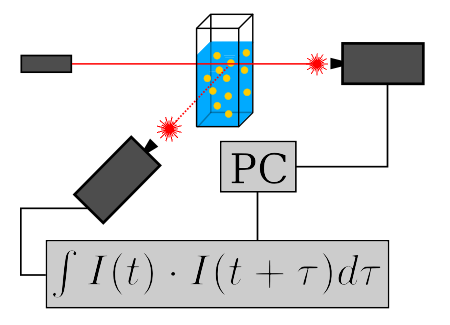
\includegraphics[width=0.8\linewidth]{./figs/chap1/dlssetup}
	\caption{}
	\label{fig:dlssetup}
\end{subfigure}
\begin{subfigure}{0.5\textwidth}
\centering
	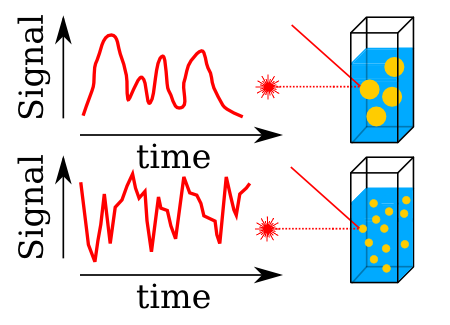
\includegraphics[width=0.8\linewidth]{./figs/chap1/dlsnoise}
	\caption{}
	\label{fig:dlsnoise}
\end{subfigure}
\caption{A schematic of a typical, simplified \dls{} set-up. Figure \ref{fig:dlssetup} shows the main components: (laser) source, sample cell, detectors, auto-correlator and a computer for data-sampling. Two detectors allow for measurement of relative intensity and thus help reduce unwanted noise from fluctuations in laser intensity. Figure \ref{fig:dlsnoise} shows how different particle sizes lead to different \enhyphen{noise} signatures in the measured signal.}
\label{fig:dlscheme}
\end{figure}
Dynamic Light Scattering (\dls{}) is most commonly used to analyse nanoparticles, specifically it can be used to determine the size of nanoparticles in solution. The optical set-up of a \dls{} experiment is shown in Figure \ref{fig:dlssetup}, a typical example of the the obtained optical signal is shown in Figure \ref{fig:dlsnoise}. A laser illuminates the sample, some amount of light is scattered by particles in solution and its intensity as a function of time is determined by the detector at an angle to the path of the laser beam. A second detector in the direct path of the light is used to subtract fluctuations in laser intensity. The \enhyphen{noise} in the measured relative intensity of the two detectors is a direct consequence of the (Brownian) motion of nanoparticles in solution and will be used to extract particle size. As particles move into and out of the path of the laser, more or less light will be scattered toward the detector. Furthermore, a particle that moves about but stays within the path of the beam for a certain delay time $\tau$ will continue to scatter light. Therefore, the evolution of the \enhyphen{noise} in time can be understood in terms of an autocorrelation function. The mathematical treatment of the signal from a population of nanoparticles with different sizes is complicated and mathematically ill posed. To overcome this difficulty experimentally, restrictions on the size distribution have to be supplied. The following discussion will be restricted to a nanoparticle population of a single size so as not to exceed the scope of this project. For such a population, the autocorrelation function
\begin{equation}
	C(\tau) = \sum _{t=0}^T I(t)\cdot I(t + \tau) \, ,
\end{equation}
where $T$ is the total time of the experiment, $I(t)$ is the intensity at time $t$ and $I(t + \tau)$ is the intensity at time $t+\tau$, will also be given by a simple exponential decay:
\begin{equation}
	C(\tau) = \exp (-2 \Gamma \tau) + B \, ,
\end{equation}
where $B$ is a baseline intensity and where $\Gamma$ is obtained by a data-fit and is related to the (translational) diffusion coefficient $D_t$ by the scattering vector $q$ as:
\begin{equation}
	\Gamma = D_t \cdot q^2 = D_t \left( \frac{4 \pi n}{\lambda} \sin \left( \frac{\theta}{2} \right) \right) ^2 \, .
\end{equation}
In the last equation $n$ is the refractive index of the medium, $\lambda$ is the wavelength of scattered light and $\theta$ is the scattering angle. Finally, $D_t$ as determined from the data-fit can be used in the Stokes-Einstein relation for Brownian motion to find the apparent hydrodynamic diameter $D_h$ of the suspended particles:
\begin{equation}
\label{diameter}
	D_h = \frac{k_B T}{3\pi \eta D_t} \, .
\end{equation}
Here, $k_B$ is the Boltzmann constant, $T$ is the thermodynamic temperature and $\eta$ is the viscosity of the suspending medium. As can easily be seen in Equation \eqref{diameter}, the determined particle diameter is directly proportional to the absolute temperature $T$, however, the viscosity of the medium is usually also very sensitively dependent on temperature and a specific value for $\eta$ needs to be supplied for the measurement. For practical purposes, the viscosity of typical (mixtures of) solvents in a range of temperatures is internally tabulated by software, as are their refractive indices. Therefore, the user of a \dls{} apparatus supplies the type of solvent used, the machine monitors the temperature during the experiment and carries out the necessary calculations and data-fitting routines. It is important to note that, for a successful size determination via \dls{}, a solution of nanoparticles should be sufficiently dilute to avoid clusters of nanoparticles while at the same time being concentrated enough to allow for measurable scattering intensities. Furthermore, the Stokes-Einstein relation assumes rigid, spherical particles so the apparent diameter of a soft, ovoid particle may significantly differ from its true dimensions.\\
The information in the presented in the preceding Section is largely based upon the presentation accompanying an advanced laboratory course taught at the Weizmann Institute of Science which is available upon request by eMail from the \href{mailto:t.bretten@gmail.com}{author}.

\section{Experimental Approach, Results and Discussion}
\label{sec:expwork}
\subsection{Sample Preparation}
\subsubsection{\sih{} Substrates}
Hydrogen passivated n-type silicon (100) with either a resistance of \SIrange{1}{4}{\ohm\metre} or a resistance of \SIrange{1}{5}{\milli\ohm\metre} is prepared according to a standard procedure: pieces of suitable size are cut from a wafers with a thickness of $\sim$\SIlist{300;500}{\micro\metre} with a diamond tip cutter, swiped off with ethyl-acetate to remove residual dust from cutting and successively sonicated for three minutes each in ethyl-acetate, acetone, methanol and water to remove organic and inorganic contaminants. Bewteen each successive sonication step, the pieces are rinsed off with the \enhyphen{new} solvent to avoid solvent cross-contamination. The pieces are microwave-treated in a plasma at \SI{100}{\watt} with a flow of \SI{1}{\cubic\centi\metre\per\minute} \oxy{} and \SI{1.5}{\cubic\centi\metre\per\minute} Ar for 3 minutes. This treatment oxidises the silicon and carbonises possible organic contaminants. Subsequently, samples are rinsed with pure water (\SI{18}{\mega\ohm\centi\metre} at \SI{20}{\degreeCelsius}) to remove residual contaminants and then immersed in \SI{2}{\percent} HF etching solution for 1 minute. The strong acid removes the oxide and creates hydrophobic \sih{} surface, which is rinsed with water to remove residual acid. The microwave treatment is repeated, the sample is rinsed again, etched again in HF and subsequently rinsed shortly to avoid possible oxidation by water. All chemicals are \SI{99.9}{\percent} purity or higher. During this process, the pieces are handled with clean plastic tweezers that underwent the same sonication steps prior to experimentation. To avoid contamination, one set of tweezers is set aside for exclusive use with HF. To avoid oxidation by air, samples are either directly further processed or stored in the inert atmosphere of a glovebox ($<\num{5}$ppm \oxy{} \& \water{}).\\
The procedure is practised until the surface layer thickness as determined by ellipsometry is reproducibly thinner than \SI{10}{\angstrom} and carrier lifetimes in high purity floatzone Si are measured at different stages during the cleaning procedure.\\
Hydrogen passivated n-type silicon (111) with a resistance of \SIrange{72}{88}{\ohm\metre} is prepared according to a similar procedure: the etch in HF is replaced by either a buffered-oxide-etch (\boe{}) or by treatment with ammonium fluoride, NH$_4$F.
\subsubsection{\pvtr{} Thin Films}
\pvdf{} thin films are spin-cast on \sih{} from solutions of different organic solvents at different concentrations ranging from \SIrange{1}{5}{\milli\gram\per\milli\litre} to investigate the influence of the solvent on thin film morphology and to allow for control over the thin film thickness. Acetone, oxygen-free dimethylformamide (\dmf{}), water-free tetrahydrofuran (\thf{}) and cyclohexanone are used as solvents. Unless otherwise noted, \SI{100}{\micro\litre} of \pvdf{} solution is pipetted onto freshly prepared \sih{} and spun for \SI{5}{\second} at \SI{500}{rpm} to distribute the solution evenly and then spun for \SI{40}{\second} at \SI{4000}{rpm} to achieve a thin film the thickness of which is determined from ellipsometry and profilometry.\\
The samples were annealed on a hotplate for different times ranging from \SI{30}{\minute} to \enhyphen{over night} at temperatures ranging from \SIrange{120}{140}{\degreeCelsius}. The samples were either heated gradually from room temperature to anneal temperature or placed on a preheated hotplate, because it was found that rapid thermal annealing may favour crystallisation of the $\beta$-phase~\cite{kang_annealspeed}. Similarly, samples were either allowed to cool gradually or thermally quenched by placing on a metal plate in an ice-bath. Poling was attempted with two different set-ups at different terminal voltages ranging from \SIrange{18}{900}{\volt} for different times ranging from \SI{30}{\minute} to \enhyphen{over night} at temperatures between room temperature and annealing temperature.\\
Poling was attempted with two set-ups one in which the \pvdf{} surface is directly contacted and one in which poling is contact-less. In the former, two series-connected \SI{9}{\volt} batteries are the voltage source. The bottom electrode is a conductive piece of copper which is connected by a screw to the source. The top electrode is a microscopy slide which is coated with a flat layer of aluminium by thermal evaporation on one side. It is contacted to the source by a strip of conductive adhesive tape. The backside of the sample is scratched, InGa eutectic is applied and the sample is firmly placed on the bottom electrode. The top electrode is placed directly onto the \pvdf{} surface and weighed down with a suitable piece of metal. Neglecting possible voltage drops in the contacts, the electrodes and the silicon substrate, this set up should develop a field of $\sim$\SIrange{1.8e7}{1.8e8}{\volt\per\metre} in the polymer layer for a polymer thickness between \SIrange{100}{10}{\nano\metre} respectively, close to or well above the coercive field strength of \pvtr{}. Simultaneous annealing and poling could be achieved, but care had to be taken to avoid burning the delicate cables. The contact-less poling device employed a high-voltage source. The bottom electrode was the same piece of copper, placed on a thick plastic insulator with a \SI{20}{\centi\metre} long vertical rod attached to it. Attached to the rod, movable along it, was a piece of insulator that had a \SI{15}{\centi\metre} by \SI{15}{\centi\metre} aluminium plate attached to it. The source was connected to the plate via an inlet for a conductive screw in the insulating holder. The surface of the aluminium could not be assumed to be flat and would therefore not serve as a top electrode directly. Thus, a silicon wafer of low resistivity was coated with a flat layer of aluminium by thermal evaporation and was connected to the metal plate with conductive paste. The top electrode assembly was lowered above the sample and the high voltage source was turned up to a value just below the electrical breakdown of air. In this manner, an electric field strength of just below $\sim$\SI{3e6}{\volt\per\metre} could realistically be achieved in the polymer layer. This is about one order of magnitude lower than the coercive field of \pvtr{}. However, even such a \enhyphen{low} electric field should induce an observable polarisation by nucleation of ferroelectric domains in \pvdf{}~\cite[pp. 812 ff.]{encyclopedia}. Specifically, Ducharme~\etal{}~\cite{ducharme_finitesize} found that nucleation processes can take place in films with a thickness $>$\SI{15}{\nano\metre} and that the coercive field falls dramatically with increased temperatures. When the phase transition temperature is exceeded during annealing and recrystallisation in the $\beta$-phase takes place inside the electric field, dipole-ordering is energetically preferred at least to some extend.\\
The \pvdf{} thin films are characterised by relative \cpd{} \& \spv{}, by \ftir{}, by the  carrier lifetimes in their substrate and their morphology is investigated by \sem{}.\\
In the majority of experiments, the samples are introduced into the antechamber of a glovebox immediate after spinning to avoid oxidation and left there under reduced pressure for for at least \SI{10}{\minute} after which the antechamber was consecutively evacuated and refilled with pure \nitro{} three times to avoid contamination of the inert atmosphere. There was concern because oxygen-levels in the glovebox reached high values, so some of the experiments were carried out in ambient atmosphere until it became clear that the solvents and procedures of this project were not the cause of the contamination in the glovebox. The initial experiments with the high-voltage poling apparatus were carried out in ambient until a sufficiently empty glovebox was found to accommodate the bulk of the apparatus.\\
\subsubsection{\pvtr{} Nanoparticles}
The synthesis of \pvtr{} nanoparticles follows the procedure described by Xiao~\etal{}~\cite{NPsynthesis}. \pvtr{} is dissolved in acetone, a good solvent for the polymer, at a concentration of \SI{5}{\milli\gram\per\milli\litre} and a mixture of water and methanol of 1:10 by volume is prepared. These solutions and pure acetone are placed in ice and the solutions are allowed to cool down for five minutes. \SI{2}{\milli\litre} of the \pvtr{}-acetone solution are injected into a \SI{15}{\milli\litre} centrifuge tube. \SI{0.5}{\milli\litre} of pure acetone are carefully injected from the bottom to form a buffer layer and subsequently \SI{4}{\milli\litre} of the water:methanol blend are also carefully injected from the bottom. The centrifuge tube is handled carefully so as not to disturb the sensitive layers and placed in ice. The nanoparticles are then precipitated out by centrifuging at \SI{19500}{rpm} for ten minutes at \SI{2}{\degreeCelsius}. The bottom layer containing \nps{} is transferred to a flask via a micro porous filter and refluxed at \SI{90}{\degreeCelsius} for \SI{60}{\minute}. The obtained solution contains \pvtr{} \nps{} and can be used for further experiments.\\
It was found that the time needed to transfer the prepared layers to the centrifuge should be minimised in order to obtain the smallest nanoparticle sizes from the synthesis. Ultra-high centrifuge speeds were found to impact the narrowness of the size distribution to a small extend. Centrifuging at \SI{18000}{rpm} was sufficient to obtain a population with a sufficiently narrow distribution, but the nanoparticle size was unaccountably too high.\\
The synthesis was carried out toward the end of the project and the problem with it became apparent too late to order a different polymer preparation: the ratio of polymer to co-polymer available for this project was 70:30 and therefore, its Curie-temperature is above the boiling point of any water:methanol mixture and indeed the synthesis by Xiao~\etal{} makes use of a 50:50 polymer:co-polymer mixture. \enhyphen{Refluxing} under conditions of increased pressure proved fruitless and substituting the water:methanol mixture with pure water in an attempt to boil under pressure at elevated temperatures was not feasible experimentally, because acetone would mix with pure water and no stable interface layers would form. Therefore, even though \nps{} could be synthesised, the material did not crystallise in its ferroelectric phase and the \nps{} could not usefully combined with solar cells. Possible further experimentation should use the appropriate polymer:copolymer mixture.
\subsection{Contact Potential Difference and Surface Photovoltage}
Over the course of the entire project, \cpd{} and \spv{} remained the main tool to see whether attempts at poling \pvdf{} were successful or not, mainly because of the great experimental ease and expediency with which the experiments could be carried out. Not all individual experiments will be presented here, but a summary of the main findings will be given. It has to be mentioned from the outset that during the whole project, no effects of successful poling could be shown and that no systematic variation of either poling-direction, solvents used, annealing temperatures or poling field strength could be shown and that results obtained in the literature, \eg{} by Lui~\etal{}~\cite{liu_THEpaper}, could not be reproduced. It is assumed that treatment with \pvdf{} remained ineffective because while the $\beta$-phase could be obtained, dipole-ordering of the ferroelectric domains failed. This might well be because poling field strengths were just too low.  The literature suggests that this should not have been the case~\cite{ducharme_finitesize}, or at least that \pvdf{} thin films used throughout this project should present a borderline case which might not reach full polarisation at the field strengths employed here, but which should never the less have shown \emph{some} effect of polarisation.\\
The \cpd{} and \spv{} experiments always compared poled to unpoled \pvdf{} thin films to untreated \sih{}. The low-voltage poling set-up gave \cpd{} and \spv{} results that were completely irregular. Independent of the poling direction, the \cpd{} of the \enhyphen{poled} sample could be up to $\sim$\SI{300}{\milli\volt} higher or lower than that of the unpoled sample and bore no discernible connection to the untreated \sih{} surface, either. The conclusion was drawn that the contacting top-electrode in the \SI{18}{\volt} poling set-up might have been a source of unknown contamination, even though care was taken that it would only ever come in contact with \enhyphen{clean} \pvdf{} surfaces and was cleaned and/or replaced by a fresh electrode from time to time. For that reason, the switch to the non-contacting poling set-up was done, even if that set-up would provide lower poling field-strengths.\\
Initial experiments with the high-voltage, no-contact set-up showed similar variations as before, this was then ascribed to acetone being a poor solvent for creation of \pvdf{} thin films and a switch to \dmf{} solvent was made. With this set-up the \spv{} of samples with the ferroelectric polymer varied around that of untreated \sih{} to within experimental uncertainty: the \spv{} of \enhyphen{poled} and unpoled \pvdf{} samples was \SIrange{14}{32}{\milli\volt} compared to \SI{20+-10}{\milli\volt} for fresh \sih{} surfaces. The \cpd{} of the \pvdf{} samples was now systematically lower than that of untreated \sih{}, with a difference ranging from \SIrange{50}{250}{\milli\volt}, depending on the exact thin film deposition method. The greatest difference in \cpd{} between untreated reference and \pvdf{} samples was found when samples were annealed at \SI{135}{\degreeCelsius} for more than \SI{30}{\minute} and when they were subsequently quenched on ice prior to poling. The difference between \enhyphen{poled} and unpoled \pvdf{} surfaces never exceeded the experimental uncertainty and the direction of the difference could not be changed by reverse-poling, either. Therefore, a switch of solvents used for \pvdf{} was again made, from \dmf{} to cyclohexanone, based on clues found in the literature~\cite{naber_cyclo}. At the same time, it was realised that \pvdf{} films might be too thin for the employed poling field strengths to be effective, so \enhyphen{thicker} solutions of \pvdf{} were employed and the speed of the spin cast was reduced from \SI{4000}{rpm} to \SI{3000}{rpm} and poling was carried out at elevated temperatures below $T_C$.\\
With these measures, the \cpd{} of samples with a polymer top layer was \SI{230+-40}{\milli\volt} below that of untreated \sih{} and there was a \SI{15+-5}{\milli\volt} difference between the \enhyphen{poled} and unpoled \pvdf{} samples, which could be switched in direction by reverse poling in three experiments, but the effect could not always be reproduced. This is an unexpected result which can only be explained if it is assumed that \enhyphen{poling} failed during the entirety of this project and that the influence of \pvdf{} on the work function of the silicon substrate is not due to its macroscopic or microscopic ferroelectric field, but due to some chemical effect of the polymer on the silicon surface.
\subsection{Ellipsometry and Profilometry}
The ellipsometer is an FQTH-100 by J. A. Woodlam Co. It is calibrated with a silicon/silicon-oxide standard. The model is silicon of appropriate thickness (\SI{500}{\micro\metre} for most wafers) plus a Cauchy-layer with thickness set as a fitting parameter. The spectroscopic scan is done over \num{100} means. The profilometer is a Dektak XXX.
\subsubsection{\sih{}}
Five pieces of \sih{} n-type silicon (100) were prepared according to the standard procedure and the thickness of their surface layer was measured at three points per piece by ellipsometry. The thickness was \SI{7+-2}{\nano\metre}, which is consistent with clean, hydrogen passivated silicon. The same procedure was carried out for n-type silicon (111), hydrogen terminated by BOE, thickness \SI{10+-1}{\nano\metre}, and for n-type silicon (111), hydrogen terminated by NH$_4$F, thickness \SI{12+-1.5}{\nano\metre}. Where ever possible, n-type silicon (100)was preferred as a substrate because of these results.
\subsubsection{\pvdf{} Thin Films}
Three thin film samples each of \pvdf{} from solutions of \SI{1}{\percent} by weight in acetone and \dmf{}, spun \SI{500}{rpm} for \SI{5}{\second} and \SI{4000}{rpm} for \SI{40}{\second} and annealed at \SI{135}{\degreeCelsius} for \SI{30}{\minute} were investigated by ellipsometry. Their thickness was \SI{17+-2}{\nano\metre} and \SI{20+-3}{\nano\metre} respectively. Solutions of \SIlist{1.3;2.5;5}{\milli\gram\per\milli\litre} \pvdf{} in cyclohexanone were likewise prepared and their thickness by ellipsometry was \SIlist{2.6+-0.1;4.6+-0.1;10.7+-0.2}{\nano\metre} respectively. Scratches were applied to the samples to reveal the underlying substrate and the height of the scratch was measured my profilometry. The measured thickness agreed to that found by ellipsometry to within \SI{3}{\nano\metre}.
\subsection{Lifetimes}
\subsubsection{\sih{}}
To assess the quality of the hydrogen passivation, carrier lifetimes in high quality n-type floatzone silicon were compared at different stages during the cleaning procedure. The minority carrier lifetimes in six individual pieces cut from the same wafer and lifetimes were measured \enhyphen{as -is}, \ie{} without any treatment just after cutting, after the first oxidation step and directly after the final chemical etch with HF. The results, summarised in Table \ref{tab:sihlifetimes}, show there are no systematic problems with the substrate preparation procedure, at least as far as minority carrier lifetimes are concerned. The variation in lifetimes after the final processing step is relatively higher than for the other stages, but is still sufficiently small so as to be no sign for concern about the quality of the passivating layer.
\begin{table}
\centering
\caption{Average minority carrier lifetimes and their standard deviations recorded from six individual pieces of n-type silicon at different stages during the cleaning procedure: 1) \enhyphen{as-is}, 2) after chemical rinsing and oxidation and 3) immediately after the final HF etch.}
\label{tab:sihlifetimes}
\begin{tabular}{@{}llll@{}}
\toprule
 & \multicolumn{3}{c}{Stage during processing} \\ \cmidrule(l){2-4} 
 & \multicolumn{1}{c}{1)} & \multicolumn{1}{c}{2)} & \multicolumn{1}{c}{3)} \\ \midrule
minority carrier lifetime (\si{\micro\second}) & \num{12+-1} & \num{3.53+-0.05} & \num{163+-19} \\ \bottomrule
\end{tabular}
\end{table}
\subsubsection{\pvdf{} Thin Films}
In a very similar experiment, the influence of \pvdf{} on the minority carrier lifetimes was investigated. The main interest was to compare poled and unpoled \pvdf{} to test the hypothesis that the electric field of the ferroelectric would reduce surface charge recombination. One piece of silicon was left untreated, \ie{} hydrogen passivated but was left on the hotplate alongside the pieces with a \pvdf{} top layer to account for possible effect of heating. This reference was also exposed to ambient for the same time that it took to spin cast \pvdf{} to account for oxidation. Finally, one piece of silicon was prepared with a surface layer of poly-methylmethacrylate (\pmma{}) to yield a sample with a comparable polymer surface layer. Four suitable pieces of silicon were cut, the two with the lowest carrier lifetimes were chosen for the untreated \sih{} reference and the \pmma{}. \sih{} was prepared according to the standard procedure, \pmma{} was spin cast onto a fresh \sih{} surface from a solution of \SI{0.3}{\milli\gram\per\milli\litre} \pmma{} in \thf{} at \SI{500}{rpm} for \SI{5}{\second} and \SI{4000}{rpm} for \SI{1}{\minute}. The sample was annealed on a separate hotplate inside the glovebox for \SI{10}{\minute} at \SI{80}{\degreeCelsius}. \pvdf{} thin films were spin cast onto fresh \sih{} from a solution of \SI{1}{\percent} by weight of \pvdf{} in acetone, spun at \SI{500}{rpm} for \SI{5}{\second} and \SI{4000}{rpm} for \SI{40}{\second}. \pvdf{} was annealed at \SI{130}{\degreeCelsius} for \SI{10}{\minute} inside the glovebox. One sample was poled using the \SI{18}{\volt} setup over-night, one sample was left unpoled. Lifetimes were measured the next day. The minority carrier lifetime in the untreated sample had decayed to \SI{12.8}{\micro\second}, comparable to lifetimes measured in untreated Si-wafers that have a natural oxide layer. The lifetimes in the poled and unpoled \pvdf{} samples were virtually identical: \SI{9.22}{\micro\second} and \SI{9.3}{\micro\second} respectively. Lastly, the \pmma{} sample had a surprisingly high lifetime of \SI{67}{\micro\second}.\\
The conclusion has to be that poling \pvdf{} prepared in this way has no effect on minority carrier lifetime and that the presence of any \pvdf{} even degrades the surface carrier recombination rates. \pmma{} seemed to have shielded the underlying substrate from residual \oxy{} in the glovebox.\\
For lack of time, minority carrier lifetime experiments were not repeated with the insights gained from the \cpd{} experiments, \ie{} thicker layers of \pvdf{} prepared from cyclohexanone solution were not investigated for their lifetimes.

\subsection{Scanning Electron Microscopy}
\subsubsection{Influence of Solvent on Thin Film Morphology}
Thin films were spin cast on cleaned indium tinoxide (\ito{}) from \SI{5}{\milli\gram\per\milli\litre} \pvdf{} in cyclohexanone and from \SI{3}{\milli\gram\per\milli\litre} \pvdf{} in \dmf{}, compared in Figure \ref{fig:semsolvent}. Samples were annealed at \SI{135}{\degreeCelsius} for \SI{30}{\minute} and the \pvdf{} was carefully scratched in some places to assure presence of polymer under the \sem{}. The substrate was placed inside a holder which electrically contacts both the substrate backside as well as the exposed \pvdf{} front surface and were introduced into a Field Emission \sem{} manufactured by JEOL, model JSF-7000F connected to and operated by the manufacturer's specific software. The acceleration voltage was \SI{5}{\kilo\volt} and the magnification was 25-times. The film morphology obtained from cyclohexanone, Figure \ref{fig:semCYCLO} is very homogeneous. The more conductive \ito{} surface appears darker in the image and serves as proof that polymer is indeed present in the image. Apart from the scratch, the coverage is complete. The individual bright spots are interpreted as dust particles from unusually long exposure to ambient. The scale-bar is invisible against the background of the sample, but is is the same as in Figure \ref{fig:semDMF}, as evidenced from the microscope's log-files. \dmf{} leads to rough, uneven \pvdf{} layers with speckles and folds, as can clearly be seen in Figure \ref{fig:semDMF}. The observations made here are in accordance with the literature~\cite{naber_cyclo}.
\begin{figure}
\begin{subfigure}{1\textwidth}
\centering
	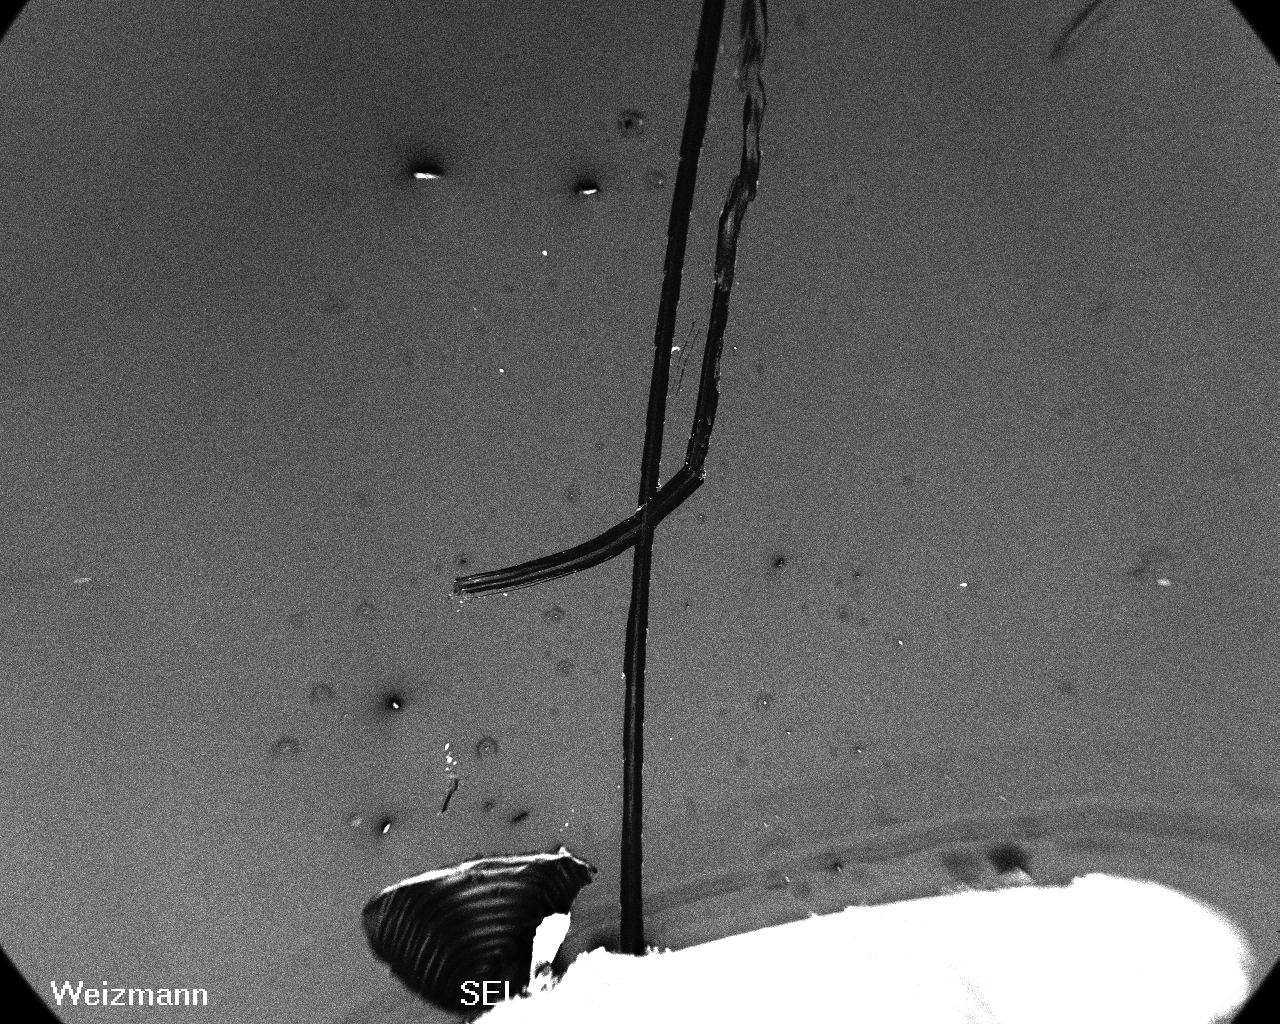
\includegraphics[width=0.9\linewidth]{./figs/chap1/semCYCLO}
	\caption{cyclohexanone solution}
	\label{fig:semCYCLO}
\end{subfigure}
\vspace{30pt}
\begin{subfigure}{1\textwidth}
\centering
	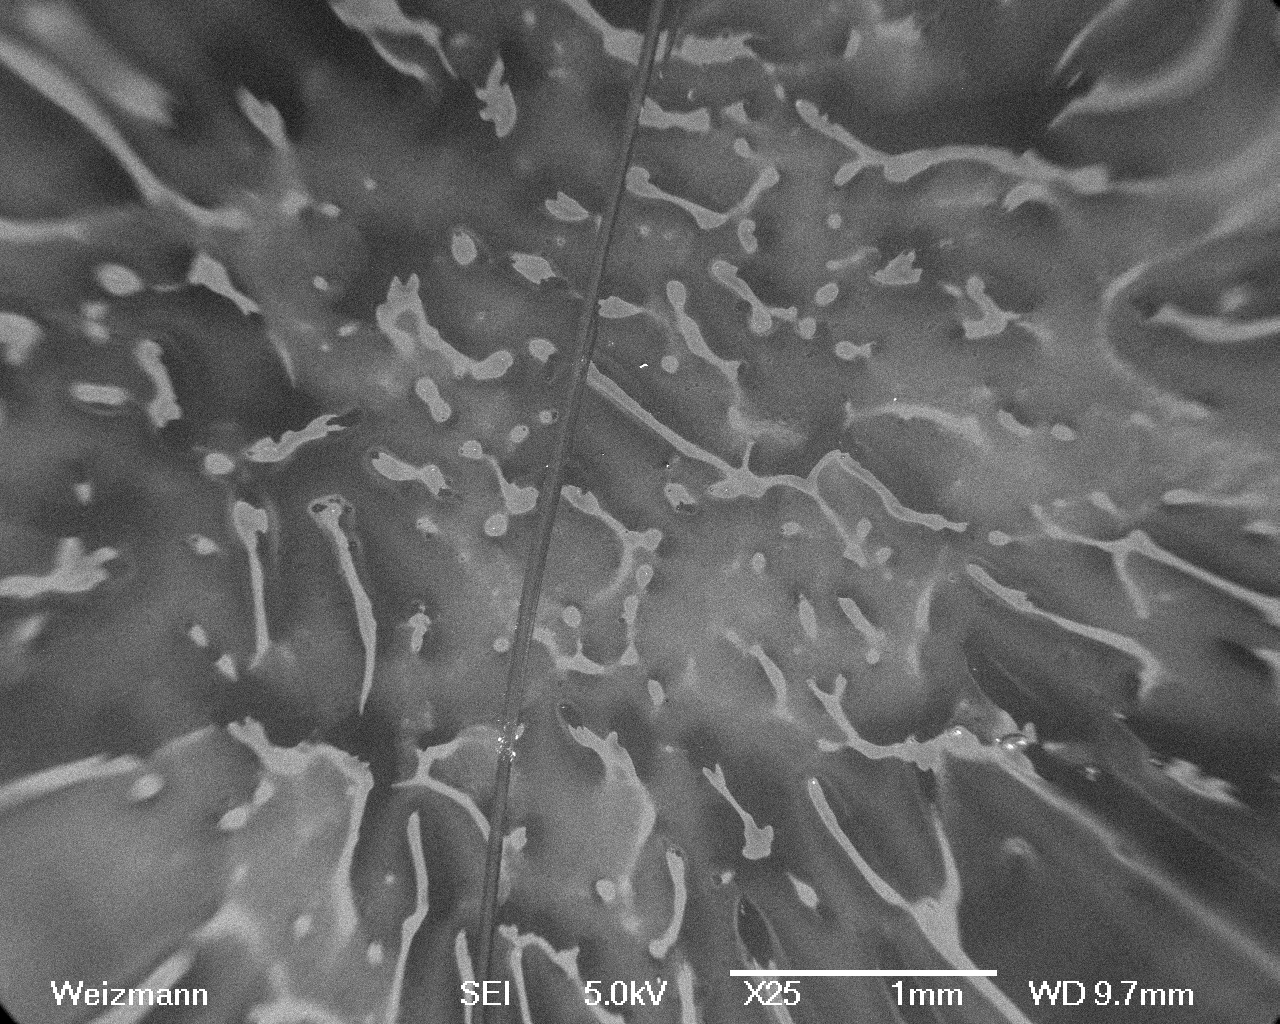
\includegraphics[width=0.9\linewidth]{./figs/chap1/semDMF}
	\caption{\dmf{} solution}
	\label{fig:semDMF}
\end{subfigure}
\caption{\sem{} images comparing the \pvdf{} thin film morphologies obtained from spin casting of different solutions.}
\label{fig:semsolvent}
\end{figure}
\begin{figure}
\begin{subfigure}{1\textwidth}
\centering
	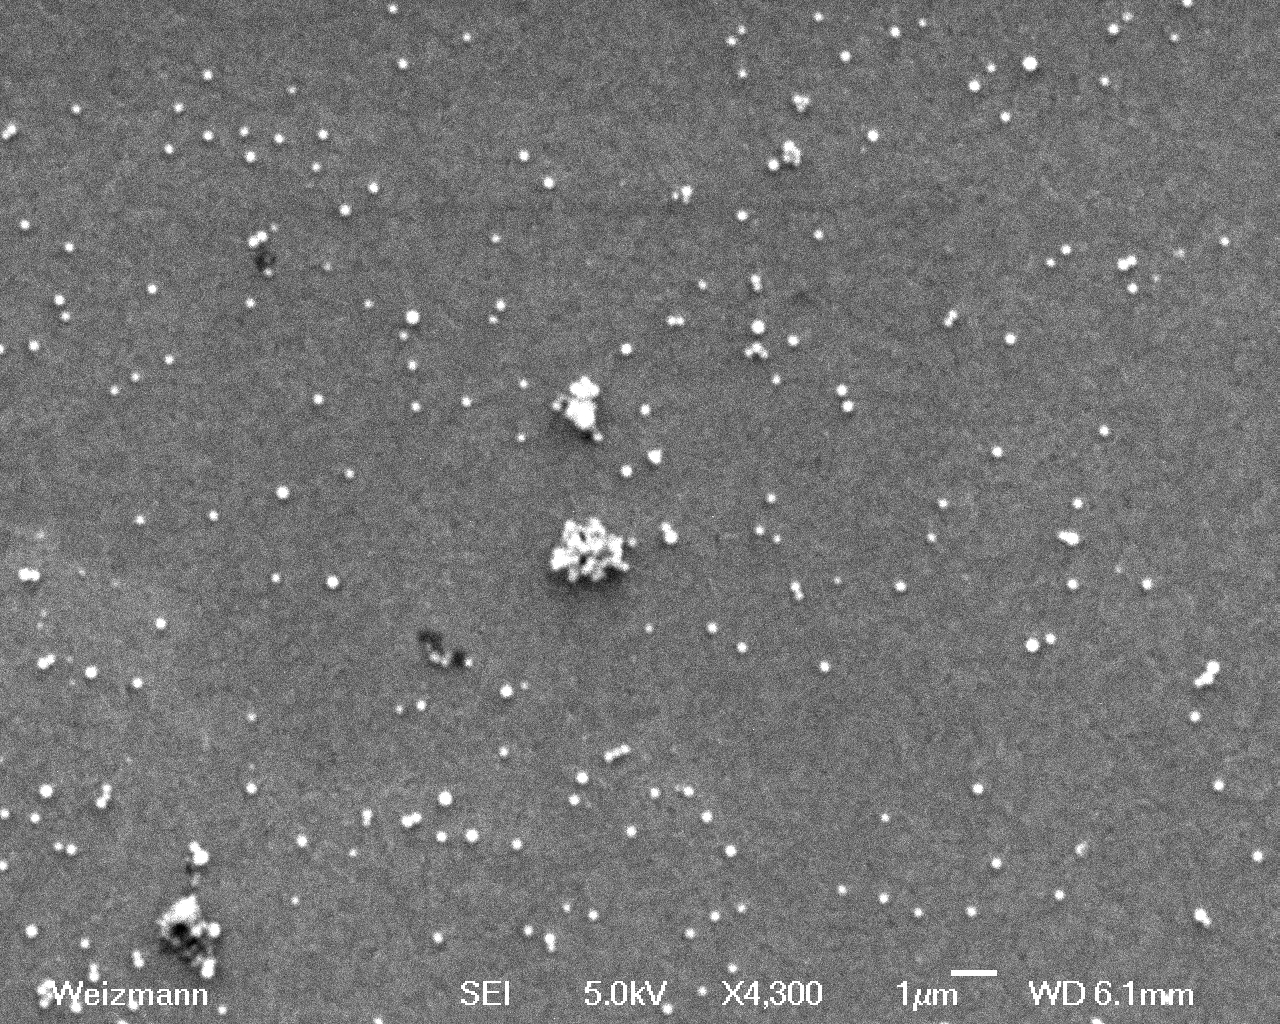
\includegraphics[width=0.9\linewidth]{./figs/chap1/semTYPNANO}
	\caption{Typical \pvdf{} \nps}
	\label{fig:semtypnano}
\end{subfigure}
\vspace{30pt}
\begin{subfigure}{1\textwidth}
\centering
	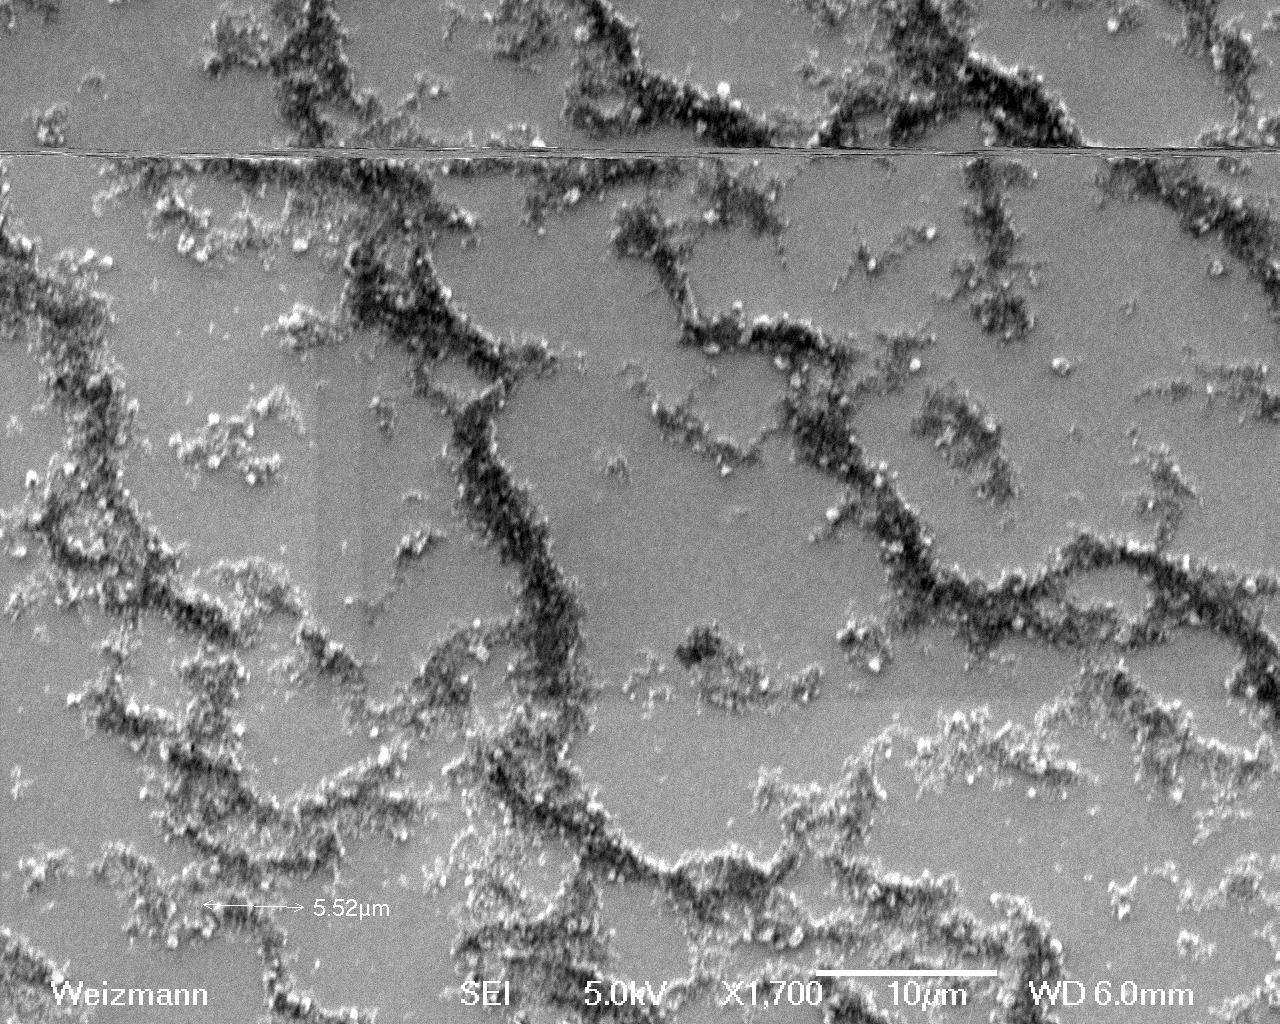
\includegraphics[width=0.9\linewidth]{./figs/chap1/semNANOSOUP}
	\caption{Amorphous structures after annealing on the substrate.}
	\label{fig:semnanosoup}
\end{subfigure}
\caption{\sem{} images comparing \enhyphen{normal} \pvdf{} \nps{} to those that were annealed at $T_C$ on a substrate.}
\label{fig:semnps}
\end{figure}

\subsubsection{Nanoparticle Characterisation}
Nanoparticle suspension was pipetted onto a cleaned \ito{} surface and the solvent was either allowed to evaporate naturally or in one case the sample was heated to annealing temperature (\SI{135}{\degreeCelsius}). The \ito{} substrates were introduced into the \sem{} in the same manner as the thin film samples. \sem{} was mainly used as a tool to determine the diameter of synthesised \nps{}. In total 23 individual \nps{} from four individual batches of synthesis were measured. The very first batch was discarded because the \enhyphen{nano}particles had an average size of $\sim$\SI{0.9}{\micro\metre}. This was because instead of directly precipitating by centrifuge, the layered solutions were left standing in the lab for $\sim$\SI{10}{\minute}. The results of the measurements of the subsequent batches are given in Table \ref{tab:npsize}. It is interesting to note that both the average size as well as the variation in the population decrease with increasing experimental experience~\footnote{The batches are numbered as successive syntheses,\ie{} b$_1$ was the first (not discarded) synthesis, b$_4$ the last that was investigated with \sem{}}. This is mainly due to faster processing of the individual synthesis steps and because later syntheses were carried out closer to the centrifuge to minimise the time the layers stay in contact without being centrifuged. The particles are about twice as big as those obtained by Xiao~\etal{}~\cite{NPsynthesis}, however, it is not immediately apparent from their paper if they used \np{} radius or \np{} diameter as a measure of size. It is assumed that diameter was used, just as in this project. Their population size distribution is narrower: standard deviation $\sim$\SI{12}{\nano\metre} compared to \SI{14}{\nano\metre} in this project's \enhyphen{best} synthesis. This may be because the centrifuging speeds for this project were instrumentally limited to \SI{18000}{rpm} instead of the prescribed \SI{20000}{rpm} or maybe because they measured \num{71} individual \nps{} instead of the five individual \nps{} in batch b$_4$.
\begin{table}
\centering
\caption[Nanoparticle diameters as obtained by \sem{}. Batches b$_1$ through b$_3$ were refluxed before size determination, batches b$_1$ \& b$_2$ were centrifuged at \SI{16500}{rpm}, b$_3$ \& b$_4$ at \SI{18000}{rpm}.]{Nanoparticle diameters as obtained by \sem{}. Values for Xiao~\etal{} are estimated from~\cite[Figure 1f)]{NPsynthesis}. Batches b$_1$ through b$_3$ were refluxed before size determination, batches b$_1$ \& b$_2$ were centrifuged at \SI{16500}{rpm}, b$_3$ \& b$_4$ at \SI{18000}{rpm}.}
\label{tab:npsize}
\begin{tabular}{@{}lcllll@{}}
\toprule
 					& \multicolumn{5}{c}{\np{} diameter (\si{\nano\metre})} \\ \cmidrule(l){2-6} 
Batch designation 	& Xiao \etal{} 	& b$_1$  & b$_2$ & b$_3$ & b$_4$ \\ \midrule
 					&  		& 290 	& 174 	& 188 	& 133 	\\
 					&  		& 263 	& 155 	& 129 	& 166 	\\
 					&  		& 198 	& 147 	& 167 	& 145 	\\
 					&  		& 283 	& 153 	& 124 	& 148 	\\
					&  		& 382 	& 229 	& 152 	& 164 	\\
 					&  		& 270 	&		& 185 	&  		\\
 					&  		& 198 	&  		& 		& 		\\ \midrule
Mean 				& 75 	& 270 	& 172 	& 157 	& 151	\\
Standard Deviation 	& 12 	& 63 	& 34 	& 27 	& 14		\\ \bottomrule
\end{tabular}
\end{table}
\sem{} was also used to try to establish the overall morphology of the \nps{}, see Figure \ref{fig:semnps} for an overview of encountered structures. Figure \ref{fig:semtypnano} shows a typical \sem{} image of the \nps{} synthesised in this project. Overall, they are roughly spherical, evenly distributed and show only few clusters. Some other \sem{} images did not show clusters at all. Lastly, it was mentioned that the \np{} dispersion could not be refluxed at a sufficiently high temperature to obtain the correct crystallographic phase. It was therefore attempted to \enhyphen{anneal} the \nps{} after being spun cast onto a substrate. The result is seen in Figure \ref{fig:semnanosoup}: unsurprisingly, the \nps{} melted and formed amorphous structures on the substrate.

\subsection{\dls{} and \np{} Size Distribution}
Dynamic light scattering measurements to characterise the size distribution of synthesised nanoparticles was carried out in a Zetasizer Nano ZSP, at room temperature. Because of its experimental ease and expediency, \dls{} was used to characterise nearly every single batch of synthesised \nps{}, until the experimental procedure was sufficiently practised to obtain \nps{} of reproducible size distributions. The nanoparticles could be taken directly from suspension and no further preparations were needed to measure \dls{}. The size distributions obtained from the Zetasizer usually showed more than one characteristic peak, but in all cases, \enhyphen{unrealistic} peaks could be identified and appropriate restrictions on the distributions as laid out in Section \ref{sec:dlstheo} could be found. Not all those individual characterisations will be shown, instead Figure~\ref{fig:dlsmeas} compares the population size distributions for \nps{} precipitated into pure water and that of \nps{} precipitated into a water:methanol mixture of 1:10 by volume. Normal distributions that characterise the nanoparticle size distributions were calculated from the histogram data. For the nanoparticles precipitated into the water:methanol blend, a size of \SI{164+-26}{\nano\metre} is obtained, while precipitation into pure water yielded \nps{} with a diameter of \SI{220+-54}{\nano\metre}. These observations are in line with those obtained from \sem{}: the \nps{} are about a factor $\sim$2 larger than what was expected from the literature, as is their size variance, but these factors may be explained by the limited centrifuging speeds available or by a misunderstanding of the definition of \enhyphen{size} employed by Xiao~\etal{}~\cite{NPsynthesis}.
\begin{figure}[h]
\centering
	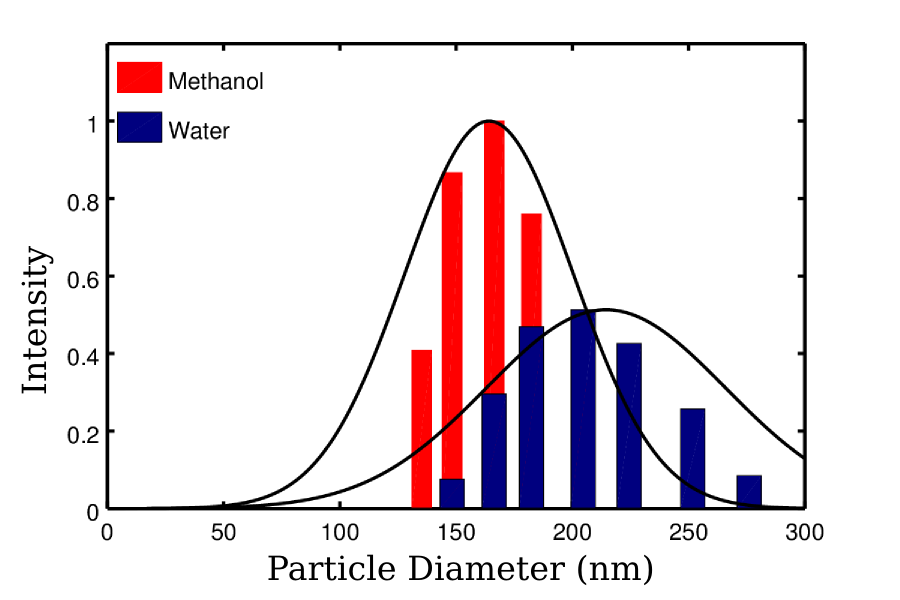
\includegraphics[width=0.9\textwidth]{./figs/chap1/dlscompare}
	\caption{Comparison of \dls{} data for \nps{} precipitated into pure water and a water:methanol mixture of 1:10 by volume. Normal distributions are calculated from the histogram data.}
	\label{fig:dlsmeas}
\end{figure}
\subsection{\ftir{} Spectra of \pvdf{} Thin Films and Nanoparticles}
\sisetup{per-mode = reciprocal-positive-first}
\ftir{} spectra were obtained using a ThermoScientific Nicolet 6700 FT-IR in \atr{} \ftir{} configuration. Thin films were spin cast from a solution \SI{50}{\milli\gram\per\milli\litre} \pvdf{} in cyclohexanone at \SI{500}{rpm} for \SI{5}{\second} and \SI{3000}{rpm} for \SI{55}{\second} and annealed at \SI{135}{\degreeCelsius} for \SI{30}{\minute} in the glovebox. Poling was attemped using the \SI{18}{\volt} set-up for one hour, also in the glovebox. The reference was a freshly prepared \sih{} surface. Nanoparticles were taken from suspension by repeatedly applying solution to an oxidised silicon surface and allowing the liquid to evaporate naturally. The reference was an oxidised silicon surface. Reference \ftir{} spectra for $\beta$-phase \pvdf{}, poled and unpoled, can be found in the literature~\cite{liu_THEpaper}. The spectra are shown in Figure \ref{fig:irplot}. The transmittance value is arbitrary and the obtained spectra were shifted to be displayed well alongside each other and the positions of the characteristic peaks are indicated by dashed lines.\\
\begin{figure}
\centering
	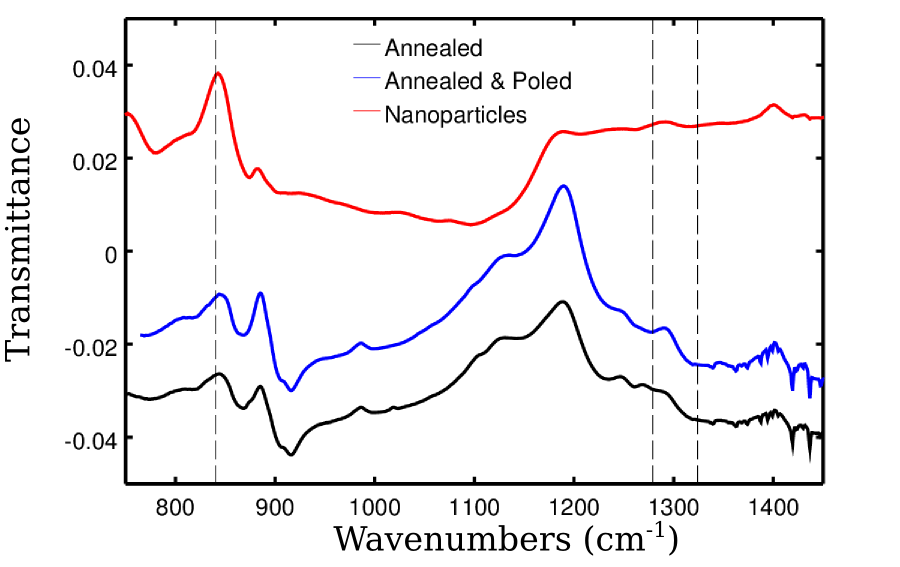
\includegraphics[width=0.9\textwidth]{./figs/chap1/IRplot}
	\caption{\ftir{} spectra of \pvdf{} in different configurations. The positions for peaks characteristic of the ferroelectric $\beta$-phase are indicated by dashed lines.}
	\label{fig:irplot}
\end{figure}
The characteristic peaks at \SIlist{1279;1324}{\per\centi\metre} less well developed than what is expected from the literature, but the overall shape of the thin film spectra still indicates presence of the $\beta$-phase of \pvdf{}. The more pronounced peaks at \SIlist{1274;1288}{\per\centi\metre} in the poled thin film compared to the unpoled thin film and their ratio compared to the highest peak at $\sim$\SI{1190}{\per\centi\metre} may be taken as an indication of polarisation of the ferroelectric perpendicular to the substrate~\cite{mao_optim}. The nanoparticles do not show features typical for the $\beta$-phase of \pvdf{}, because they could not be refluxed at sufficiently high temperatures.
\sisetup{per-mode = symbol}%


\subsection{IV Curves of c-Si/\pvdf{}/\pdot{} Schottky junctions}
\begin{figure}
\begin{subfigure}{1\textwidth}
\centering
	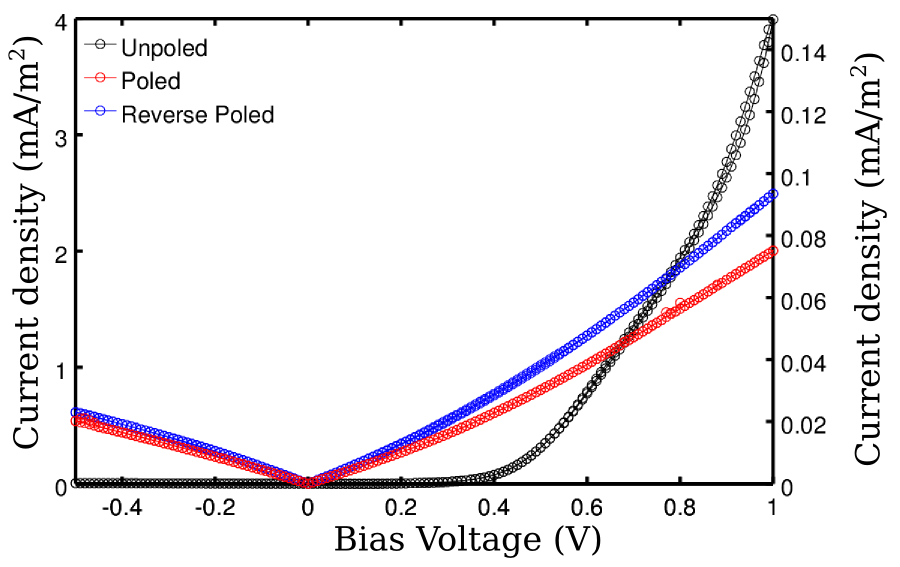
\includegraphics[width=0.9\linewidth]{./figs/chap1/IV1}
	\caption{Initial cells, exposed to ambient.}
	\label{fig:iv1}
\end{subfigure}
\vspace{30pt}
\begin{subfigure}{1\textwidth}
\centering
	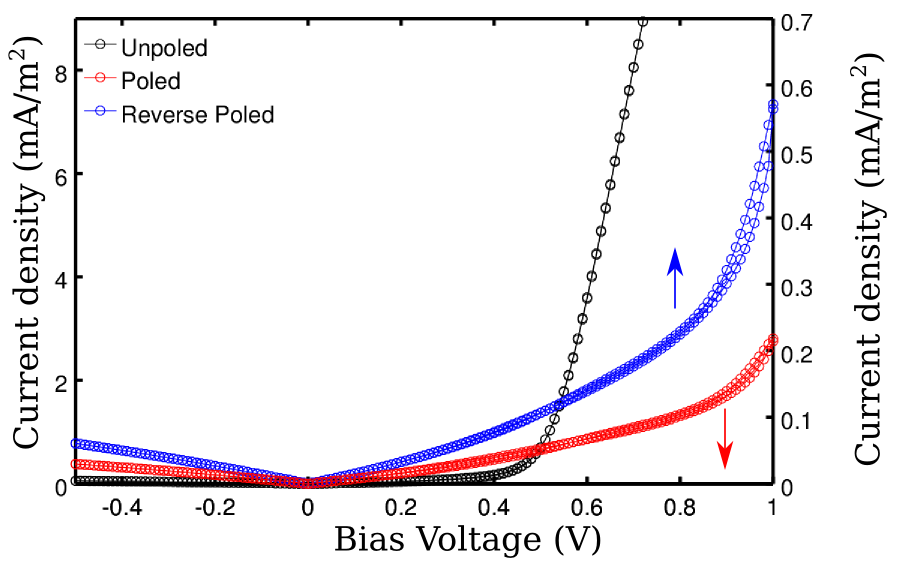
\includegraphics[width=0.9\linewidth]{./figs/chap1/IV2}
	\caption{Exposure to ambient minimised.}
	\label{fig:iv2}
\end{subfigure}
\caption[IV curves obtained for unpoled, poled and reverse poled \sih{}/\pvdf{}/ \pdot{} Schottky junction solar cells.]{IV curves obtained for unpoled, poled and reverse poled \sih{}/\pvdf{}/\pdot{} Schottky junction solar cells. Note that the poled and reverse poled cells are plotted on their own y-axis, the one at the right side of the Figures.}
\label{fig:iv}
\end{figure}
Ferroelectrically assisted solar cells, \ie{} Schottky junctions, were created from a silicon substrate obtained via the standard procedure. \pvdf{} was spin cast at \SI{500}{rpm} for \SI{5}{\second} and \SI{3000}{rpm} for \SI{55}{\second} from a solution of \SI{1}{\milli\gram\per\milli\litre} \pvdf{} in cyclohexanone. \pvdf{} was annealed at \SI{138}{\degreeCelsius} for \SI{30}{\minute} in the glovebox. A \pdot{} layer on top of the ferroelectric was spin cast for \SI{1}{\minute} at \SI{1000}{rpm} from a solution of \SI{6}{\milli\litre} \pdot{} stock with \SI{0.057}{\gram} ethyldiglycol (\edg{}) and \SI{0.004}{\gram} of Zonyl surfactant in \SI{2}{\milli\litre} water. \pdot{} was annealed \SI{140}{\degreeCelsius} for \SI{30}{\minute} in the glovebox. Top electrodes were thermally evaporated from high purity Ag at a rate of \SI{2}{\angstrom\per\second} for \SI{100}{\second} at manual settings. The back contact of the junction was created by scratching with a diamond tip and applying InGa eutectic. Polymer was scratched off the substrate to obtain a rectangular active area, the size of which was determined with optical microscopy. Poling was attempted via the solar cells top and bottom electrodes using two series-connected \SI{9}{\volt} batteries. In the first experiment, four cells were characterised with IV immediately after evaporation. Because of experimental and time limitations, the \enhyphen{best} cell was chosen and left over-night. The next day, it was characterised by IV to gain a measure for its degradation in the glovebox over night. The cell was then poled for \SI{1}{\hour} and was characterised by IV, reverse-poled for \SI{1}{\hour} and characterised again. Poling was done in ambient. The IV curves are shown in Figure \ref{fig:iv1}. Th cell degraded in ambient and lost its rectifying characteristics, currents decreased by a factor $\sim$40.\\
The same experiment was repeated, but cell-processing, characterisation, poling and reverse poling were all carried out in one day and exposure of the cells to air was minimised by poling \& reverse poling inside the glovebox. Defining \& measuring the cell area, creating a back contact and characterisation still exposed the cells to ambient. The IV curves are shown in Figure \ref{fig:iv2}. The poling procedures reduced the cell current by a factor $\sim$90.\\
The reason the cells degraded to such an extend is obvious in hindsight. The poling procedure exposed the cells to a positive bias of \SI{18}{\volt} and the batteries and cell were connected in series to the back- and front contacts of the cell. A constant current of relative high magnitude was therefore lead through the cells for an hour. Care should have been taken to limit the degrading currents through the cell. It is surprising that the \enhyphen{poled} cells in the second experiment still show any rectifying behaviour at all and that the poling direction still influenced the current through the cells. An influence of the ferroelectric properties of \pvdf{} on the behaviour of inversion-layer solar cells could therefore be shown to a minute extend, but the effect could not be used to achieve the goal of this project, namely to \emph{enhance} solar cells.  

\newpage
\section{Discussion and Conclusion}
Two critical sources for the understanding of this project, the \enhyphen{Encyclopedia of Smart Materials}~\cite{encyclopedia} and the finite size effect of on the polarisation of \pvdf{} layers~\cite{ducharme_finitesize}, were not known during the time of the actual project. Several experimental mistakes could have been avoided had that been the case. The approach of first preparing a thin film of \pvdf{} and measuring its effect on the underlying substrate proved largely fruitless. The idea was to study a simpler system first, before going on to assemble complete cells. From the available literature about cells that incorporate \pvdf{}, the conclusion was drawn, that thin films $<$\SI{20}{\nano\metre} should be investigated, but \pvdf{} films in solar cell applications are size limited because of their insulating character. Thicker films might have proven more useful for identifying an effect on the work function of the substrate, especially given the limitations imposed by the finite size effect and the available poling field strengths. The simpler poling set up making use of a contacting electrode probably suffered from contaminations, while the contact-less high voltage set up did not provide a sufficiently strong field to appreciably pole the ferroelectric. For the characterisation with \ftir{}, thicker films were employed to gain a measurable signal and poling was attempted with the contacting set up. Accordingly, some evidence of poled \pvdf{} films could be found in the \ftir{} spectra. Cyclohexanone was identified as the best solvent for obtaining homogeneous \pvdf{} thin film layers, in accordance with the literature~\cite{naber_cyclo}. Once fully assembled, a c-\sih{}/\pvdf{}/\pdot{} Schottky junction solar cell showed an effect of poling the ferroelectric. Cells could not be improved because they were subjected to high currents as a result of high positive bias for extended periods of time. This mistake is obvious in hindsight, but was not realised at the time. The \pvdf{} films employed in the cells were exceedingly thin, $\sim$\SI{1}{\nano\metre}, but poling via the front and back contacts of the cell yielded a sufficiently strong electrical field to overcome the finite size effect and induce a measurable polarisation in the films non the less.\\
Nanoparticles were synthesised from the material and characterised. They did not crystallise in the ferroelectric $\beta$-phase, because $T_C$ of the material used here was too high to allow \enhyphen{refluxing} at the necessary temperatures. This experimental oversight only became clear during an eMail a correspondence with one of the authors of the original paper by Xiao~\etal{}.\\
Future research should learn from the avoidable mistakes made here and should concentrate on the correct methods for the correct aims: if \pvdf{}'s influence on the work function is to be studied, sufficiently thick films should be employed. If the goal is to enhance solar cells, complete junctions should be assembled right away, because they provide a convenient way of poling the ferroelectric via their contacts that avoids contamination of the thin films. If contact-less poling is attempted, a method will have to be found that would allow placing the top electrode at heights above the sample in the micro-meter range. The set up used here was incapable of such precise placing and the electrical breakdown of air accordingly placed limitations on poling field strengths, ultimately rendering the set up useless for our purposes. Instead of trying to reproduce every literature result step by step using simple and successively more complex systems, the characteristics of \pvdf{} should be understood as well documented and well established by at least a whole generation of researchers. Some of those results were reproduced in this project, but because of the failures along the way, the research could not be carried on to the point of adding to the existing knowledge.

	\chapter{Temperature Dependent Surface Photovoltage}
	\label{chap:spv}
	\section{Introduction}
This Chapter deals with realising and validating an experimental set-up to measure the temperature dependent surface photovoltage (\spv{}(T)) with the help of a cryogenic system, a modified Kelvin probe (\kp{}) and a suitable source of illumination. Section \ref{sec:theo} will introduce the necessary physical background underlying the measurements with a \kp{} and will be followed by a more thorough description of the actual Kelvin probes in use in Section \ref{sec:kp}, subdivided into a description of the already established systems (Section \ref{sec:kppold}) and the \enhyphen{new} system (Section \ref{sec:kpnew}). The experimental approach described in the following Sections is aimed at validating, step-by-step that the \enhyphen{new} system reproduces results obtained with the established systems and to investigate possible complications that the capabilities of the \enhyphen{new} system might bring to light. The experimental approach will culminate in a report of a temperature dependent measurement of the \spv{} for a chosen model system in Section \ref{sec:vox}. While results obtained in that last Section cannot be fully explained at this point, the measurement did serve as a useful proof of principle to show that reproducible \spv{}(T) measurement are feasible with the system. A brief conclusion will round off this Chapter.

\section{Theory}
\label{sec:theo}
\subsection{The Contact Potential Difference and the Kelvin Probe}
When two (semi-)conductors with dissimilar Fermi levels are electrically connected from their back-side with a gap between them, charge will flow from the material with the lower work function (\wf{}) to the one with the higher \wf{}. The work function is defined as the energy needed to remove an electron from a solid to a point in vacuum immediately outside of it. Electrons will stop flowing when equilibrium is established. As long as there is a gap between the materials, an electrical field will develop in the gap due to the difference in the local vacuum level across this gap. 
The potential drop across the gap, the contact potential difference or \cpd{}. When the work functions are expressed in Electron-Volts, the \cpd{} is directly equal to the difference of the \wf{}s:
\begin{equation}
\label{wf}
	{\cpd} \, \equiv \,  \wfp \, - \wfs \, .
\end{equation}
The order of the operands in the equation above is a matter of convention. Their physical representation depends on how the measurement system which we will investigate in the following -- the Kelvin Probe -- is set up electrically. 
In the configuration outline above, the materials behave like a parallel plate capacitor and a capacitance is established, which is known to be:
\begin{equation}
\label{cap}
	C(t) = \frac{\epsilon \epsilon_0 A}{d(t)} \,
\end{equation}  
in which $\epsilon$ \& $\epsilon_0$ are the permittivity and the permittivity of free-space respectively, $A$ is the area of the parallel plate and $d(t)$ is the distance between the plates. $d(t)$ is taken as a function of time, because the Kelvin Probe varies the distance in time. The current between the plates is given by the change in charge on the plates, which is in turn given by the change in capacitance:
\begin{equation}
	I(t) = \frac{dQ}{dT}= \Delta V \frac{dC}{dV} \, ,
\end{equation}
where $\Delta V$ is the difference in potential between the plates, which is the sum of the applied backing voltage and the naturally occurring potential difference between the plates, the \cpd{}: $\Delta V = V_{\text{Backing}} + \cpd$. If we assume a sinusoidally varying distance with the average distance between the plates being $d_0$, $d_1$ being the amplitude of oscillation, $\omega$ being its frequency of oscillation and an arbitrary phase $\psi$, then
\begin{equation}
	d(t) = d_0 + d_1 \sin (\omega t + \psi)\, 
\end{equation}
and finally
\begin{equation}
\label{current}
	I(t,\Delta V) = -\epsilon \epsilon _0 A \Delta V \frac{d_1 \omega \cos (\omega t + \psi}{(d_0 + d_1 \sin (\omega t + \psi))^2}\, .
\end{equation}
In equation \eqref{current}, the current is written as a function of time and potential difference between the plates, because while continuously varying the distance between probe and sample, the Kelvin Probe also varies $V_{\text{Backing}}$. As can easily be seen from equation \eqref{current}, the current is zero or 'nulled' when $V_{\text{Backing}}=-\cpd$. Thus, if \wfp{} is known, \wfs{} can easily be calculated from equation \eqref{wf}. In practice, this requires calibrating the probe head against a sample with known work function, \hopg{} in the context of this study. Obviously, if one wants to study the work function of a sample as a function of temperature, the temperature dependence of the work function of the probe also has to be known. In most cases and especially for simple metals, the work function only varies over a few hundredths to a few tenths of meVs per Kelvin~\cite{tempdepmet,tempdepmet2,tempdepmet3,tempdepmet4,tempdepmet5}. These variations are negligible compared to other sources of experimental uncertainty and the work function of the probe is therefore assumed to be constant with respect to temperature throughout this work.\\
As pointed out, the work function \wf{} of a semiconductor is defined as the the energy needed to remove an electron from the material to a point in vacuum just outside of it and is given by the difference of the near surface vacuum vacuum energy $E_{\text{vac}}$ and the Fermi energy $E_{\text{f}}$ of the material: $\upvarphi = E_{\text{vac}} - E_{\text{f}}$. The Fermi level of a doped semiconductor is dependent on the temperature and the carrier-concentrations of the semiconductor and can be expressed in terms of the intrinsic Fermi energy as:\\[5pt]
\begin{minipage}[c]{0.4\textwidth}
	\begin{equation}
	\label{efn}
	E_{f,n} \, =  E_i \, - \, kT \ln{\frac{n}{n_i}}
	\end{equation}
\end{minipage}	
\hfill
and
\hfill
\begin{minipage}[c]{0.4\textwidth}
	\begin{equation}
	\label{efp}
	E_{f,p} \, = E_i \, + \, kT \ln{\frac{p}{p_i}}
	\end{equation}
\end{minipage}\\[5pt]
for n- and p-type semiconductors respectively. As can be seen from the preceding equations, $E_{f}$ changes with the Boltzmann Temperature. At 300 K~\footnote{approximately room temperature} and at 100 K, $kT$ is approximately equal to 26 and 8.6 meV, respectively. In many cases, it is assumed that the extrinsic carrier concentrations $n$ and $p$ are equal to the product of dopant concentration and number of supplied free carriers per dopant atom. But even in that case, the concentration of intrinsic carriers is still a strong function of temperature and requires knowledge of several material parameters to calculate precisely. A simpler argument that is valid for moderately doped semiconductors in which the Fermi-Dirac distribution can be approximated by the Boltzmann distribution is developed in the following for the example of an n-type semiconductor. In such a semiconductor, the chance of finding an electron close to the conduction band edge is greater than finding a hole close to the valence band edge. Therefore, the Fermi level is closer to the conduction band. At absolute zero, all levels below the Fermi level are filled and all levels above the Fermi level are empty, by definition. At absolute zero, there can be no free electrons as freedom to move would imply energy. Therefore, at absolute zero, the Fermi level cannot be above the conduction band edge. So far, it is shown that the Fermi level must be closer to the conduction band, but below its band edge. At extremely high temperatures, doping will be negligible because thermally generated carriers will exceed carriers introduced by the dopant. Therefore, the Fermi level will tend toward the intrinsic Fermi level in mid gap. A similar argument holds for the Fermi level of a moderately doped p-type semiconductor and it is therefore shown that:\\[5pt]
\begin{minipage}[c]{0.4\textwidth}
	\begin{equation}
	\frac{dE_{f,n}}{dT} < 0
	\end{equation}
\end{minipage}	
\hfill
and
\hfill
\begin{minipage}[c]{0.4\textwidth}
	\begin{equation}
	\frac{dE_{f,p}}{dT} > 0
	\end{equation}
\end{minipage}\\[10pt]
for the Fermi level of an n-type and a p-type semiconductor, respectively.
\subsection{The Surface Photovoltage and Band Bending}
In the context of this work, the surface photovoltage (\spv{}) is defined as the \cpd{} measured under illumination minus the \cpd{} in the dark:
\begin{equation}
\label{spv}
	\spv \equiv \cpd_{\text{light}} - \cpd_{\text{dark}} \, .
\end{equation}
\begin{figure}
\begin{subfigure}{0.5\textwidth}
\centering
	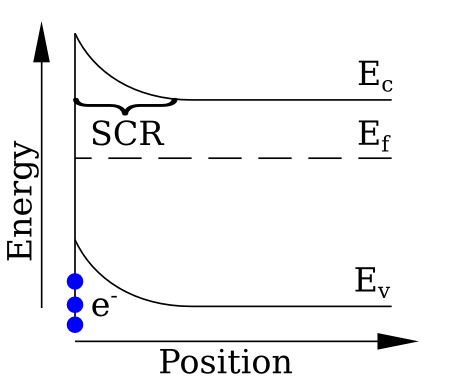
\includegraphics[width=0.8\linewidth]{./figs/bb-dark}
	\caption{}
	\label{fig:bbdark}
\end{subfigure}
\begin{subfigure}{0.5\textwidth}
\centering
	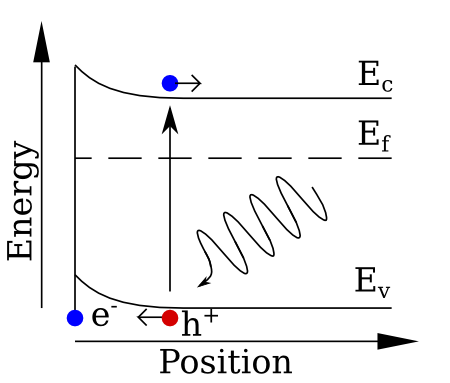
\includegraphics[width=0.8\linewidth]{./figs/bb-light}
	\caption{}
	\label{fig:bblight}
\end{subfigure}
\caption{Band bending, trapped surface charges and the space charge region at the surface of an n-type semiconductor (a) in the dark and (b) under illumination. Note the decrease in trapped surface charges in (b) and the resulting reduction in band bending. Energy levels of the valence band, $E_v$, the Fermi level, $E_f$, and the conduction band, $E_c$, are included for reference.}
\label{fig:bb}
\end{figure}
It is instructive to refer to the diagrams in Figure \ref{fig:bb} to understand the origin of the surface photovoltage: in the dark, majority carriers are trapped at the surface, setting up a space charge region (\src{}). For n-type semiconductors, electrons are in the majority, accumulating negative charge on the surface, setting up an electrical field pointing from the bulk toward the surface. This field causes the potential energy of electrons to be higher at the surface than in the bulk and accordingly, the bands in Figure \ref{fig:bbdark} are bent 'up'. Of course, the situation is reversed for p-type semiconductors. Under illumination, electron-hole pairs are created where radiation of sufficient energy is absorbed. For direct band-gap semiconductors, the absorption depth is shallow and electron-hole pair generation might well occur within the \src{}. For indirect band-gap materials, absorption might occur deep within the bulk and carriers might have to diffuse through the material until they reach the \src{}. Regardless of their path, once the carriers are close to or within the \src{} the direction of the electrical field present there causes minority carriers to be attracted to the surface and majority carriers to be repulsed back to the bulk. Once the minority carriers reach the surface, they will recombine with majority carriers already present there. This causes the charge at the surface to decrease and the bands to flatten, see Figure \ref{fig:bblight}. When the trapped surface charge is completely neutralised, the bands will return to their initial flat state, the \src{} will vanish and it is said that the \spv{} has saturated~\cite{yates_bandbend}. Saturation is usually assumed in an experiment when a further increase in illumination intensity does not lead to a further change in observed light \cpd{}. For this reason, \spv{} is often the method of choice when investigating the band bending~\cite{macnamara_tempdepspv,macnamara_tempdepspv2} but it should be noted that in the presence of strong Fermi level pinning, bands might still be bent, even if \spv{} saturation is reached~\cite{kronik_spv}. In that case, bending is not exclusively due to trapped charges and care should be taken when analysing results obtained by \spv{}. In a metal, the Fermi level lies within the conduction band. Therefore, carriers are free to move to and from the surface and no notable \src{} will exist in a metal. Therefore, no difference in \cpd{} between the dark and the illuminated condition is expected for a metal, so equations \eqref{wf} and \eqref{spv} combine to give the \spv{} as a function exclusively in terms of the sample material:
\begin{equation}
\label{spvs}
	\spv = \upvarphi _{\text{s,dark}} - \upvarphi _{\text{s,light}} \, .
\end{equation}
To gain a deeper insight into the behaviour of a semiconductor as it reacts to light, its work function can be redefined in more practical terms, namely in terms of electron affinity, band-bending, conduction band edge and Fermi level, which are shown in Figure \ref{fig:terms}. 
\begin{figure}
\begin{subfigure}{0.5\textwidth}
\centering
	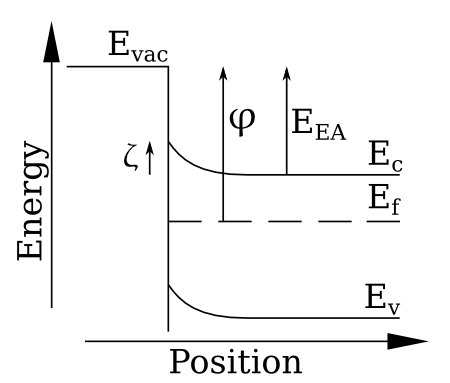
\includegraphics[width=0.8\linewidth]{./figs/bbdefn}
	\caption{}
	\label{fig:bbdefn}
\end{subfigure}
\begin{subfigure}{0.5\textwidth}
\centering
	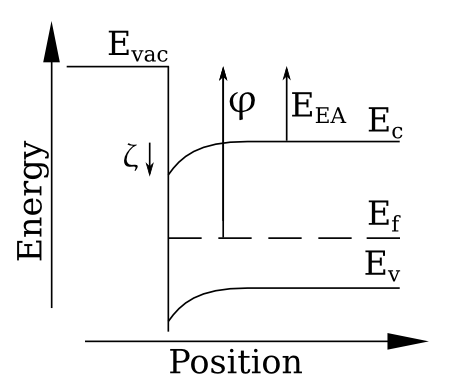
\includegraphics[width=0.8\linewidth]{./figs/bbdefp}
	\caption{}
	\label{fig:bbdefp}
\end{subfigure}
\caption{Definition of terms electron affinity, $E_{EA}$, band-bending $\upzeta$, conduction band edge, $E_c$, Fermi level, $E_f$ and work function, $\upvarphi$, for an n-type semiconductor (a) and a p-type semiconductor (b). It can be clearly seen that the band bending is negative for the p-type semiconductor. Valence band edge, $E_v$, included for reference.}
\label{fig:terms}
\end{figure}
Here, electron affinity is defined as the energy obtained by moving an electron from vacuum just outside the semiconductor to the bottom of the conduction band edge deep inside the semiconductor, which is subtly different from its usual definitions in Chemistry and Solid State Physics~\footnote{In Solid State Physics $E_{EA}$ is usually defined as the energy gained by moving an electron from vacuum just outside the material to the conduction band close to the surface, because this quantity is experimentally accessible. Our definition gives access to the band-bending,$\upzeta$, as an independent parameter.}. We have:
\begin{equation}
\label{Eea}
	E_{\text{EA}} \equiv E_{\text{vac}} - E_c \, .
\end{equation}
Band-bending, $\upzeta$, is the difference in energy of the conduction band close to the semiconductor surface and deep within the semiconductor, so the work function can be given by
\begin{equation}
\label{wfbb}
	\upvarphi = E_{\text{EA}} + E_c - \upzeta - E_f \, .
\end{equation}
In the equation above, $E_{\text{EA}}$ and $E_c$ are not affected by illumination, band-banding vanishes under saturation~\footnote{in the absence of Fermi level pinning} and $E_f$ can change because of its dependence on the carrier concentrations as expressed in equations \eqref{efn} and \eqref{efp}. However, if its change due to illumination is for the moment assumed to be small compared to the band bending, then combining equations \eqref{wfbb} and \eqref{spvs} yields an interesting property of the \spv{}: its sign can be used to identify if a sample is n- or p-type. For an n-type semiconductor, $\upzeta$ is positive and thus its \spv{} is also a positive quantity; for a p-type semiconductor, the situation is reversed: both $\upzeta$ and \spv{} are negative.


\section{Kelvin Probes in use}
\label{sec:kp}
\subsection{Established Kelvin Probe System}
\label{sec:kppold}
As mentioned, it was the aim of this project to establish if a combination of a cryogenic system fitted with a custom \kp{} probe head could be used for temperate dependent measurements of the \spv{}. The system in question will be described in detail in Section \ref{sec:kpnew}, here, the focus will be on a brief description of the two Kelvin probe system that were already established and had been in use in the Cahen group for some time.\\
Both systems feature \kp{} probe heads model \enhyphen{Kelvin Probe S}, manufactured by Besocke Delta Phi GmbH~\cite{besocke}, electrical and mechanical control is provided by systems provided by the same manufacturer. Housing and illumination for the Kelvin probe set-ups are provided by in-house built solutions. The probe head consists of a \SI{2.5}{\milli\metre} diameter opaque gold grid and as such provides a stable and inert reference surface for measurements of the \cpd{}. In practice, however, the probe heads still need to be calibrated with \hopg{} if absolute measurements of the \wf{} are desired because changes in humidity, contamination or other, unknown factors can greatly influence the work function of the probe heads.\\
The first Kelvin probe system is situated in a shielding Faraday cage placed inside a humidity controlled room (\SI{20}{\percent} relative humidity) and the probe head is exposed to ambient. This system will be referred to as the \enhyphen{Ambient Probe Station}. The sample is mounted onto a conductive block of metal which is slid into a holder that provides an electrical ground for the sample specimen. Samples are either connected with InGa eutectic via their backside or with the help of an electrically conductive clip-holder screwed to the conductive block of metal. The sample is stationary and the probe head is positioned close to the surface under investigation with the help of micrometer screw gauges. Illumination of the sample is achieved with a xenon-lamp driven by a VariAC-power source with up to \SI{60}{\watt} electrical power and an optical lens focusing the light onto the surface of the mounted sample. The illumination level is controlled manually and increased until saturation of the \spv{} signal is reached. \cpd{} data are collected with a custom LabView program and monitored in real time.\\
The second system is very similar, but is placed inside a humidity and oxygen controlled glovebox (ideally $<\num{5}$ppm \oxy{} \& \water{}) and will therefore be referred to \enhyphen{Glovebox Probe Station} or \enhyphen{Glovebox 301}~\footnote{The glovebox and its probe station are situated in room 301 on a different floor than the other experimental facilities of the Cahen group.}. Mounting and electrical connection of the sample are virtually identical to the Ambient Probe Station, but illumination offers more flexibility. On the one hand, an identical illumination set-up, also using a xenon-lamp and VariAC source can be used. On the other, the system is fitted with a more advanced illumination scheme to allow for Surface Photovoltage Spectroscopy (\sps{}) measurements over a spectral range spanning \ir{} to ultraviolet (\uv{}) radiation. These capabilities were not use in this project and so shall not be further described. For the purposes of this project, the Ambient and Glovebox probe stations are practically identical and offer a trusted source of comparison for \cpd{} and \spv{} data taken with the new, to be developed system. Influences of the atmosphere, viz. clean nitrogen vs. ambient, were investigated but were found to be negligible compared to the unavoidable experimental uncertainties in \cpd{} and \spv{} measurements.
\subsection{The Lakeshore Cryogenic System coupled with a \McA{} Kelvin Probe}
\label{sec:kpnew}
Lakeshore is an international vendor of cryogenic probe stations. For this research, a Lakeshore Model TTPX Probe Station was used. The probe station can be thought of as being divided into four components. An outer vacuum-chamber is connected to a pump to reduce the pressure inside the station. An Argon gas inlet connected to the vacuum chamber can be used to provide an inert atmosphere. Inside the vacuum chamber is a separate, smaller chamber: the radiation shielding stage, primarily used to shield the sample from \ir{} radiation and thus used to facilitate measurements at low temperatures. The radiation shielding to some extend also provides electrical shielding from stray electrical signals and can therefore act as a quasi Faraday-cage. Both these chambers are fitted with windows to allow for placement of the probe-arms and to allow for visual inspection of the experiment. The radiation shielding stage's windows is made from sapphire glass, as sapphire glass is oblique to infra-red radiation. Inside the shielding stage is placed the sample stage, which allows for mounting of samples and can provide an electrical ground. The fourth and last component of the probe station are its six probe-arms. They allow for placement of several probes on the sample from the outside. For many measurements, these probes are conceptually simple gold wires which allow for electrical measurements of the sample, such as IV and CV characterisation. Being a cryogenic system, the Lakeshore is fitted with three thermocouples. They measure the temperature of the sample stage, the radiation chamber and the probe-arm respectively. The temperature is adjusted by an electrical heater and by controlling the flow of of coolant, either liquid nitrogen or -- to achieve lower temperatures -- liquid helium. Evacuation of the cryogenic system is achieved by a combination of two pumps: a `weak pump' to reduce the pressure to $\sim$ \num{5e-2} and a \enhyphen{turbo pump} to reduce it down to $\sim$ \num{5e-4}. A schematic of the Lakeshore model TTPX cryogenic system showing its components is given in Figure \ref{fig:McAscheme}.\\
\begin{figure}
\centering
	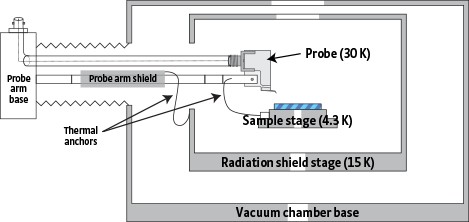
\includegraphics[width=0.8\linewidth]{./figs/Config_TTPX}
	\caption{Schematic of the Lakeshore model TTPX cryogenic system and its components, typical operational temperatures are indicated. Taken from the vendor's website~\cite{lakeshore}.}
	\label{fig:McAscheme}
\end{figure}
In our case, one of the probe arms is fitted with a modified \McA{} ultra-high vacuum (\uhv{}) Kelvin probe head. The original \McA{} \uhv{} Kelvin probe head is a horizontal base-arm ending in a vibrating, stainless steel cylinder of 2.6 mm diameter ending in a continuous, flat disk. This disk forms one of the two capacitor plates necessary for a \cpd{} measurement. The other capacitor is, of course, the sample. Using the \McA{}, the measured signal is given by equation \eqref{wf} i.e. the signal is equal to the work function of the probe head, usually $\sim$ \SI{4.5}{\electronvolt}, minus the work function of the sample. A reduction in measured \cpd{} therefore means an increase in the sample's work function.\\
The original probe head configuration is not suitable for the Lakeshore cryogenic system because the sample needs to be placed horizontally onto the sample-stage. Therefore, a vertical geometry is needed for the probe-head. Such a custom system was provided by \McA{}. The stainless-steel Kelvin probe head is now vertically mounted in a plastic base. The size and especially the weight-distribution of the original cylinder are carefully designed by \McA{} to comply with a vibration-response that is suitable for the probe head controller. The probe head is electrically connected by a gold wire that runs along the base-arm and is either soldered directly onto the cylinder or tightly wrapped around a conductive screw which is used to hold the probe head in place in its plastic holder. In the latter case, conductive silver paste suitable for \uhv{} environments is applied to the screw to ensure low resistance electrical connection. Contact potential difference measurements are severely negatively affected by non-ohmic back contacts. A second probe arm of the cryogenic system was fitted with an optical fibre to allow for laser illumination of the sample. However, in practice, it quickly became clear that such an illumination set-up was unsuitable for \spv{} measurements. This was due to several reasons. For suitable \cpd{} measurements, the probe head needs to be brought in very close proximity to the sample: distances on the scale of a few hundred micrometers are often necessary to obtain a sufficiently noise-free signal~\footnote{This adds to the practical danger of involuntarily crashing the vibrating probe head onto the sample, potentially damaging the sample, contaminating the probe head and generally interfering with conducting an experiment}. Therefore, there is simply not enough room for the exit of the optical fibre to be placed in a position where light would illuminate the sample. A further difficulty of the fibre illumination scheme are noticeable reductions in light intensity due to absorption in the fibre. After all, the fibre needs to be able withstand vacuum conditions and low temperatures, limiting the choice of suitable materials. Lastly, the fibre would provide a very localised spot of illumination. For a successful measurement of the \spv{}, the whole area under the probe head has to be saturated by illumination at the very least. Full saturation of the whole sample surface is in most cases desirable to suppress unwanted carrier recombination in the dark areas. For these reasons, it was decided to modify the probe head and employ a different illumination scheme. The cryogenic system's windows allow for illumination by a source of light placed outside the vacuum chamber, on top of the external window, focused onto the sample surface. To allow this scheme to work, the main body of the probe head needed to be hollowed out and holes needed to be drilled into the head's disk to let light pass through and onto the sample. Such a probe head, manufactured from stainless steel, was provided by \McA{} and used in initial experiments. When successful measurements were not forthcoming, three further modifications of the probe head were tried, all based on the same principle. The idea was to replace the massive disk with a wire-grid used for transmission electron microscopy (\tem{}). Three different types of wire-grids were purchased from Structure Probe Inc., a stiff, stainless steel grid with \SI{70}{\percent} opacity, two thin, flexible gold grids with \SIlist{70;60}{\percent} opacity respectively. The grids were laser-welded onto custom-made, hollowed out stainless steel cylinders. These new probe heads were manufactured by the Weizmann Institute's Department for Construction and Engineering. Care was taken to ensure acoustic vibration characteristics of the new probe heads were similar, if not identical to those of the original \McA{} probe heads. The wire-grids would add two benefits: they would increase the overall transmission of the probe head as well as allow for a more even illumination of the sample surface. In practice, however, no immediate, significant difference between the performance of the original hollow stainless steel probe head and the new, \tem{} wire-grid heads was found. At this point, an inherent limitation of the adopted illumination scheme has to be pointed out: namely that even in the ideal case, illumination from above will only result in an illuminated area directly under the probe head. The probe arm, probe head holder and even the edge of the hollow cylinder will all cast a a shadow on the sample, especially since they need to be placed directly above it.\\
\begin{figure}
\centering
	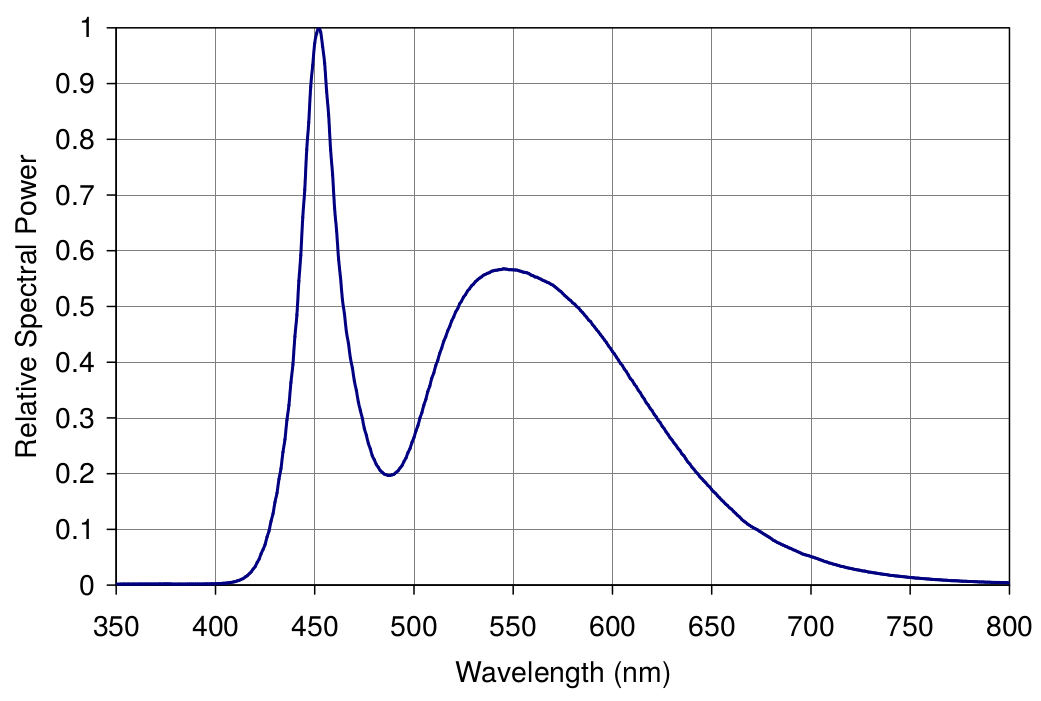
\includegraphics[width=0.8\linewidth]{./figs/ledspec}
	\caption{Typical relative spectral intensity of the LEDengine LED at an operating temperature of 25\degcent{}, taken from the vendor's supplementary information~\cite[p. 10]{ledengin}.}
	\label{fig:ledspec}
\end{figure}
In order to allow for saturating illumination of the sample, the choice of light source is crucial and it was thus a main focus of this part of the project to identify such a source and to successfully connect it to the combination of Lakeshore cryogenic station and \McA{} Kelvin Probe. Successful \spv{} measurements are routinely carried out in the group using the Ambient Kelvin Probe Station and its xenon-lamp. The xenon-lamp is not only a source of light, but also a source of heat and thus unsuitable for the temperature-dependent measurement inside the \McA{}. Not only would the heat introduce uncertainties in temperature but temperature gradients introduced by it could also damage the cryostation, specifically the radiation shielding stage's sapphire window. Therefore, the choice fell upon a high intensity, natural-white light emitting diode (\led{}) manufactured by \led{} Engin, model LZP-00CW0R. The LEDEngin \led{} uses 25 \led{}-spots soldered onto and electrically connected by a printed circuit board (\pcb{}). Using thermo-paste, the \led{} is mounted onto a copper-core of a discarded computer fan. The fan is driven by a motor that uses a small 12V AC current source to achieve the necessary cooling of the delicate \led{}. As purchased, the \led{} has a relatively wide illumination cone of \ang{60}, due to an internal fish-eye lens that is situated right atop the \pcb{}. Therefore, the lamp was supplemented by a total internal reflection lens by LEDEngin that focuses \SI{90}{\percent} of the illumination into a \ang{10} wide cone. The initial \led{} of nominally \SI{4200}{\lumen} intensity was damaged, only 12 of 25 \led{}-spots were functioning and was later replaced by new \led{} of the same manufacturer with \SI{5400}{\lumen} intensity. The \led{} is driven by a variable DC source at a maximum voltage of \SI{18.2}{\volt} and maximum current of \SI{1.5}{\ampere}. Its relative spectral intensity is given in Figure \ref{fig:ledspec}.


\section{Measuring \cpd{} at room temperature}
\subsection{Sample Preparation}
A fresh surface of \hopg{} is prepared by gently rubbing adhesive tape onto a square piece of \hopg{} and tearing it off evenly. The piece is mounted onto a sample-holder using an electrically conductive clip and the \cpd{} is measured.\\
n-\sih{} (100) with different resitivities/doping-levels is prepared according to a slightly modified standard cleaning procedure: pieces of suitable size are cut with a diamond tip cutter, swiped off with ethyl-acetate and successively sonicated for three minutes each in ethyl-acetate, acetone, methanol and water. The pieces are microwave-treated in an \oxy{}-plasma at \SI{100}{\watt} with a flow of \SI{1}{\cubic\centi\metre\per\minute} \oxy{} and \SI{1.5}{\cubic\centi\metre\per\minute} Ar for 3 minutes. Subsequently, samples are rinsed with pure water (\SI{18}{\mega\ohm\centi\metre} at \SI{20}{\degreeCelsius}), immersed in \SI{2}{\percent} HF etching solution for 1 minute, rinsed with water and ashered again as before. The pieces are etched as before, back-contacts are created by applying InGa-eutectic to a scratched back surface. The piece is mounted onto a sample holder and the \cpd{} is measured for at least two minutes each on three different spots per piece. The time the sample is subjected to ambient after etch and before each measurement is recorded and used in a linear fit \lq{}$\Delta (\cpd{})/\Delta \, t$\rq{} to serve as an indication of the \cpd{} each spot on each piece would have had right after the etch, i.e. without the time needed for creating the back surface, mounting the sample and measuring other spots.
\subsection{Results \& Discussion}
The standard deviation of measured \cpd{} between spots of the same piece is comparable to that between pieces, so all obtained values were averaged. The values obtained across the three systems agree very well with each other and in the case of mid- and high-resistivity silicon also with theory, see Figure \ref{fig:nsih}. A three,  instead of only one, minute long HF etch did not influence the \cpd{} obtained for the low resistivity sample. A possible explanation for the deviation from theory might be found in the increased surface-reactivity of highly doped silicon: by the time the experiments are started, the silicon surface might already be oxidised. 
\begin{figure}
\centering
	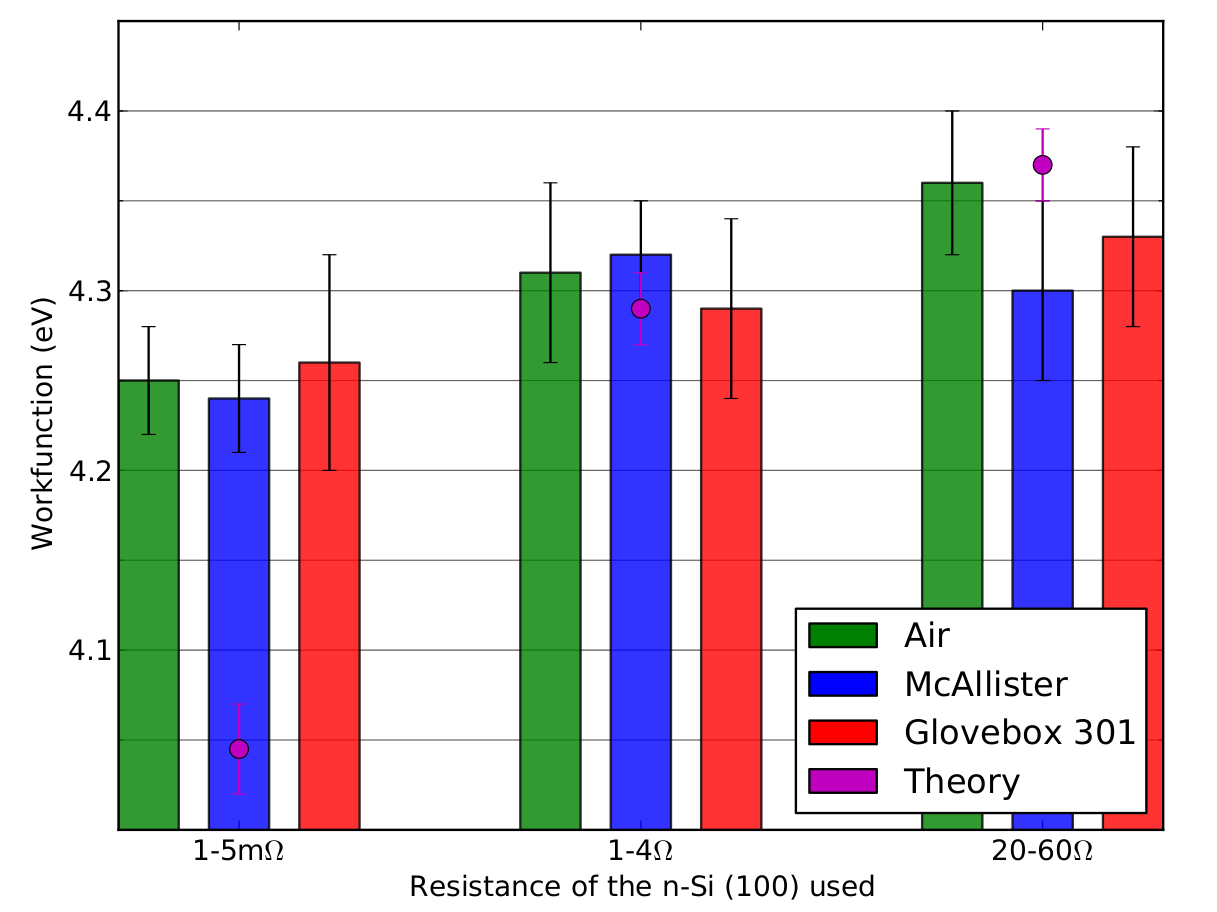
\includegraphics[width=0.8\textwidth]{./figs/Sih}
\caption{Summary of the calculated work functions for the n-\sih{} samples used. There is good agreement between the different systems and good agreement with theory, except for the case of low resistivity, highly doped silicon. Indicated errors include deviations in the samples \& the inaccuracy of calibration with \hopg{}.}
	\label{fig:nsih}
\end{figure}


\section{\cpd{} as function of pressure and temperature}
\subsection{\cpd{} as a function of pressure}
Once it was established that results obtained from the three independent system under similar conditions using hydrogenated silicon as a reference sample, efforts were concentrated on temperature and pressure dependent measurements in the Lakeshore cryogenic system. Because of unavoidable contamination with oxygen from ambient, hydrogenated silicon was not used to that end. Instead, a freshly prepared reference of \hopg{} was placed on the ground of the radiation shielding stage without a sample-mount. An electrically conductive screw and clip were used to connect the top of the \hopg{} sample to the electrical ground of the Lakeshore. Two sets of experiments were carried out to independently determine the influence of pressure and temperature on the measured \cpd{}. In the first set, the measurements was commenced under ambient condition and allowed to continue for some time. The probe head was then retracted to avoid crashing it onto the sample and the weak pump was turned on. The probe head was then brought into proximity of the sample to continue the measurement and the measurement was allowed to continue for some time. The probe head was retracted again and the turbo pump was switched on. Again, the probe head was lowered to continue with the measurement and the measurement was allowed to continue for some time. For results of this experiment, see Figure \ref{fig:hopg-p}.
\begin{figure}
\begin{subfigure}{0.5\textwidth}
\centering
	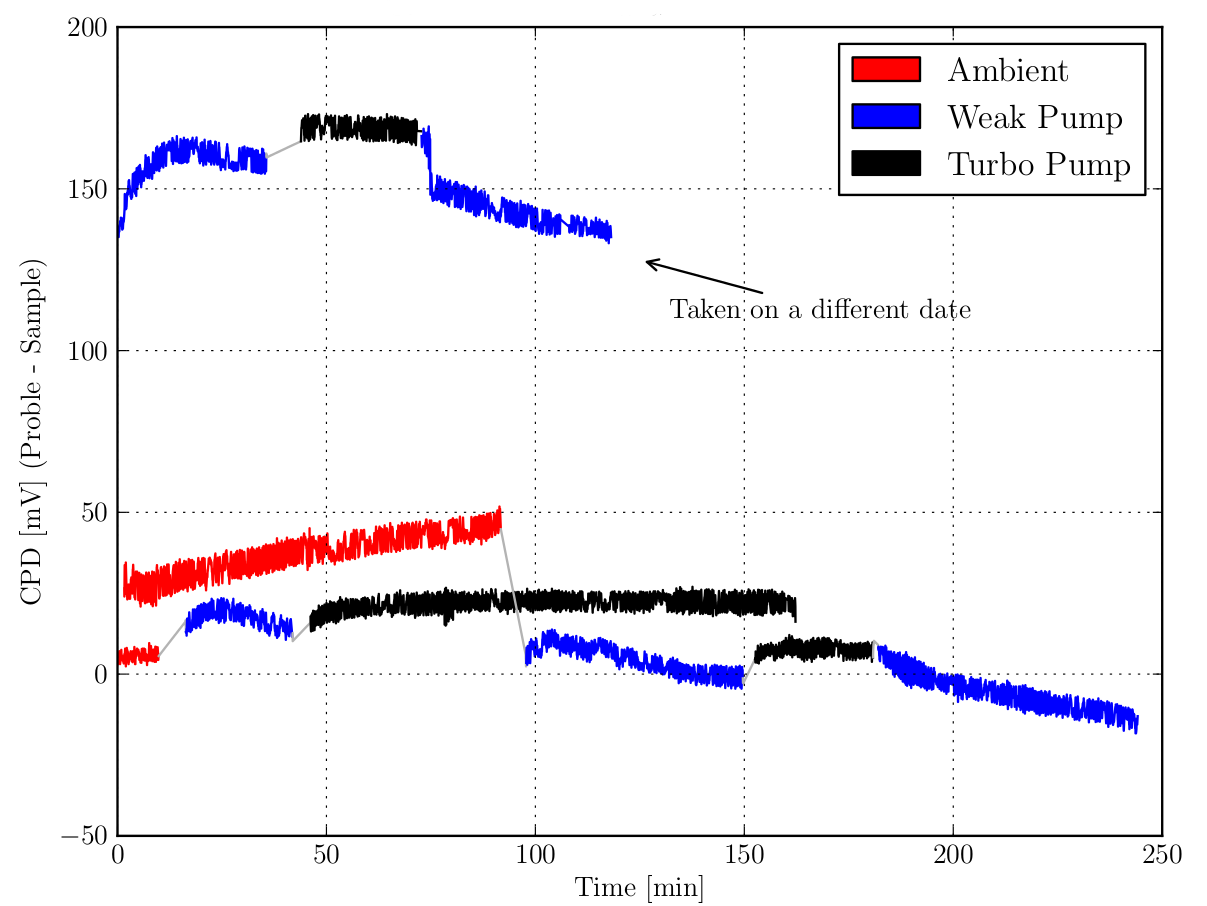
\includegraphics[width=0.95\linewidth]{./figs/HOPGMcA}
	\caption{}
	\label{fig:hopg-p1}
\end{subfigure}
\begin{subfigure}{0.5\textwidth}
\centering
	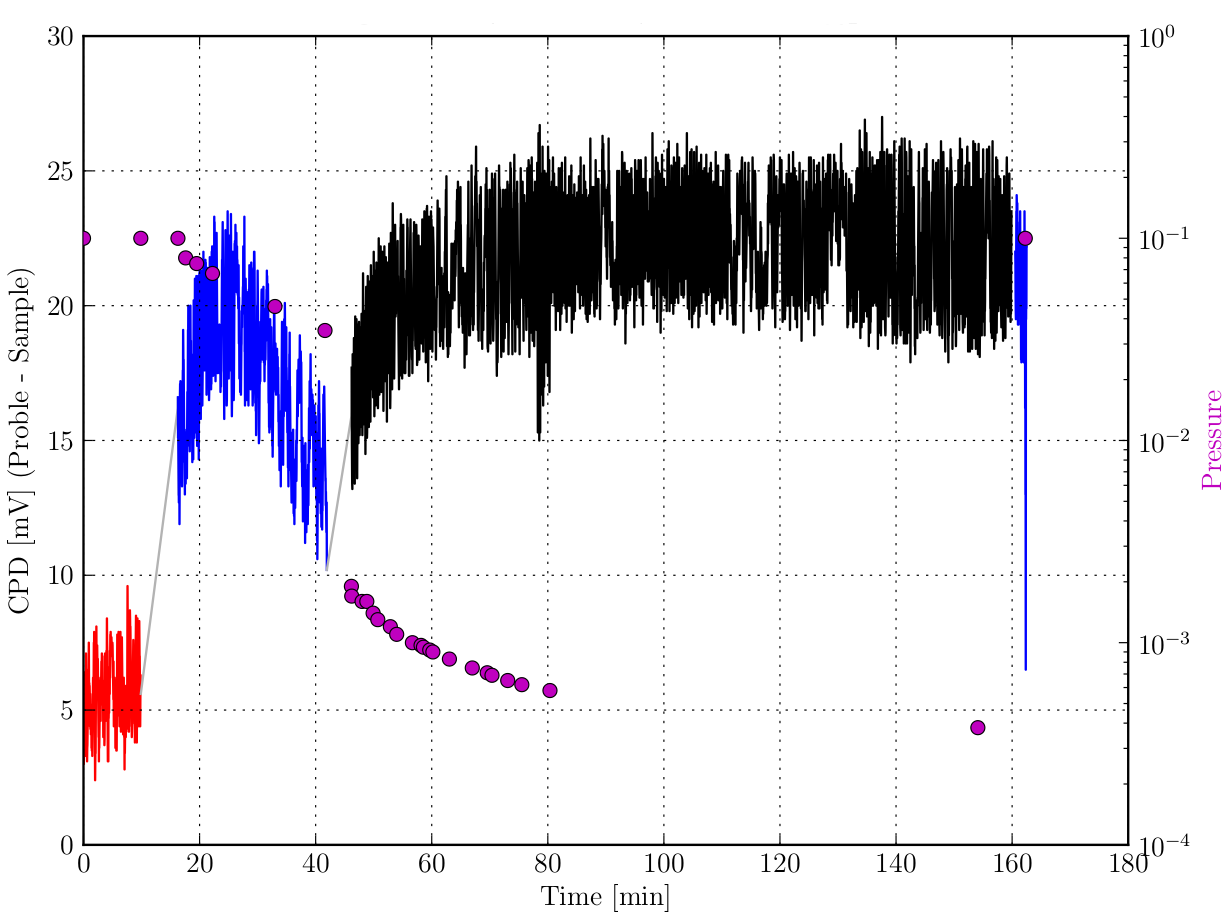
\includegraphics[width=0.95\linewidth]{./figs/HOPGMcAPres}
	\caption{}
	\label{fig:hopg-p2}
\end{subfigure}
\caption{Raw data obtained from a measurement of the \cpd{} during pressure reduction in the \McA cryogenic system. Figure \ref{fig:hopg-p1} shows results obtained from independent measurements of a piece of \hopg{} carried out on different days. It is indicated which pump was active to reduce the pressure inside the sample chamber. Figure \ref{fig:hopg-p2} gives more detail about one of these measurements and actual measurements of the pressure at different stages during evacuation.}
\label{fig:hopg-p}
\end{figure}
This experiment revealed several features. Firstly, the \cpd{} of \hopg{} rises as a function of time under ambient condition. This is readily explained by oxygenation and/or other sources of contamination from ambient, such as water for example. Once the weak pump is turned on, there is a discontinuity in \cpd{}. This discontinuity is not systematic in its direction, it may change the \cpd{} either 'up' or 'down' and can therefore best be explained by a displacement of the probe head over the sample. The sudden reduction in pressure exerts a force on the probe arm and may cause it to move slightly. The size of the discontinuity is within the size of variation of \cpd{} observed when different spots of the same reference are measured. The \cpd{} now reduces as a function of time and this may be explained by gradual decontamination of the sample: as the pressure reduces, previously adsorbed contaminants may leave the surface. A second viable explanation may be a gradual change in acoustic vibration characteristics as a result of the reduction in pressure. To distinguish between the two, an experiment was performed in which the sample chamber was flushed with clean, inert Argon after having been subjected \uhv{} conditions for about 20 minutes. It is assumed that complete desorption of possible contaminants is achieved by this treatment and that the high purity argon does not introduce fresh contaminates. The pressure was then again reduced using the weak pump and the \cpd{} again reduces as a function of time. We therefore conclude that the observed reduction in \cpd{} is indeed caused by gradual changes in pressure rather than desorption of contaminants. It is thus advisable to carry out \cpd{} experiments under conditions of stable pressure, especially given the fact that the probe head is specifically designed by \McA{} to carry out ultra-high vacuum \cpd{} measurements. 
\subsection{\cpd{} as a function of temperature}
To determine the possible influence of temperature on the quality and reliability of the measurement, an ultra-thin layer of aluminium was deposited onto a piece of silicon by atomic-layer-deposition and a natural layer of surface oxide was formed. Alumina was chosen as a surface of interest because of its natural affinity for water. If contamination by water and subsequent freezing of the surface is an inherent problem of low temperature \cpd{} measurements, then a strongly hydrophilic surface should exhibit these problems. A fresh wafer of silicon with \SI{20}{\nano\metre} of aluminium by \ald{} was cut into suitable pieces. Pieces were swiped off with ethyl-acetate and sonicated for three minutes in iso-propanol, blow-dried under \nitro{} and subsequently microwave-treated in an \oxy{}-plasma at \SI{100}{\watt} with a flow of \SI{1}{\cubic\centi\metre\per\minute} \oxy{} and \SI{1.5}{\cubic\centi\metre\per\minute} Ar for 3 minutes, ensuring a clean alumina surface. The back-side was scratched and InGa-eutectic was applied to create a back-contact. The work-function of this surface was measured in the ambient probe station and found to be \SI{4.0+-0.12}{\electronvolt}. To ensure an ohmic back-contact, the sample stage of the Lakeshore was lightly scratched and a small quantity of InGa-eutectic was applied to the stage. The piece was then placed on the sample stage and slight pressure was applied. The stage was introduced into the Lakeshore cryogenic system and the pressure was reduced. Using liquid nitrogen and the heaters, the temperature was reduced to \SI{250}{\kelvin} and allowed to stabilise. Under these conditions, the work-function of the alumina surface was found to be \SI{4.17+-0.15}{\electronvolt}~\footnote{A suitable piece of \hopg{} was also present in the sample chamber to allow for calibration of the work-function of the probe head}. It has to be pointed out that the sample surface is not the coldest point inside the Lakeshore's inner chamber. Because of the way liquid nitrogen is introduced into the system, the radiation chamber's ground surface is the coldest. Therefore, it can be assumed that any ice would form there rather than on the sample, corroborating the result presented above.
\subsection{Conclusion}
\cpd{} measurements using the Lakeshore are feasible when the pressure is constant. They may be carried out under ambient pressure with an inert argon atmosphere or under ultra-high vacuum conditions. A changing pressure is not conducive for reliable measurements of the contact potential difference but under conditions of stable pressure, \cpd{} values obtained from the Lakeshore agree with values obtained from the other probe stations. Lowering the temperature below the freezing point of water does not pose an inherent restriction on the feasibility of \cpd{} measurements in the Lakeshore system. The observed \cpd{} was in agreement with experiments carried out at room temperature. In agreement with the literature~\cite{tempdepmet,tempdepmet2,tempdepmet3,tempdepmet4,tempdepmet5} possible fluctuations of the work function of the probe head are small compared to other sources of experimental uncertainty and the \wf{} can indeed be taken as a constant.


\section{Measuring the \spv{} at room temperature}
A necessary condition for the successful determination of the \spv{} of a sample is saturation with light. In practice, this means that the light-intensity during a measurement of the \spv{} is gradually increased up to the point where further increase in intensity does not lead to further increase of the measured surface photovoltage. Detailed interpretation of the measured signal is often problematic and requires intimate knowledge of the sample and even theoretical discussions of the \spv{} tend to be very involved. However, from the point of view of establishing whether a new experimental set-up is suitable for more advanced \spv{}-measurements, a successful, saturated measurement of the \spv{} of a relatively simple test-sample is a necessary precondition. To that end, \spv{} measurements of an alumina surface were chosen as a test case. Alumina was chosen for its stability, relative simplicity and because of its relatively large \spv{} signal. The sample is the same as used for the determination of the temperature dependence of the \cpd{}: 20 nm aluminium deposited by \ald{} onto a wafer of silicon. The preparation and cleaning protocol of the sample is the same as above: rinsing; sonication; oxidation and creation of an ohmic back-contact using InGa-eutectic. The sample's \spv{} was determined in the ambient probe station as is~\footnote{i.e. ambient probe station and xenon light source} and was found to be \SI{530+-20}{\milli\volt}. To check if the \led{} is a suitable source, it was installed in the ambient probe station and an \spv{} measurement was carried out. To facilitate the comparison between the systems, the ambient probe station's light focusing lens was removed as no such lens could readily be installed with the Lakeshore. Since the \led{} has a variable electrical source, it was possible to increase the current through the \led{} from \SIrange{1}{1.6}{\ampere} in steps of \SI{0.1}{\ampere}. In a set of preliminary experiments not reported here, it was established that the illumination intensity of the \led{} as determined from a standard silicon test-cell does indeed increase smoothly over the appropriate current range when combined with the Kelvin probe stations as described. The sample was introduced into the Lakeshore's inner chamber and the \led{} was placed on top of the vacuum chamber's outer window. The current through the \led{} was increased in the same steps as for the measurement in ambient and the results of the experiment are summarised in Figure \ref{fig:Iseries}.
\begin{figure}
\centering
	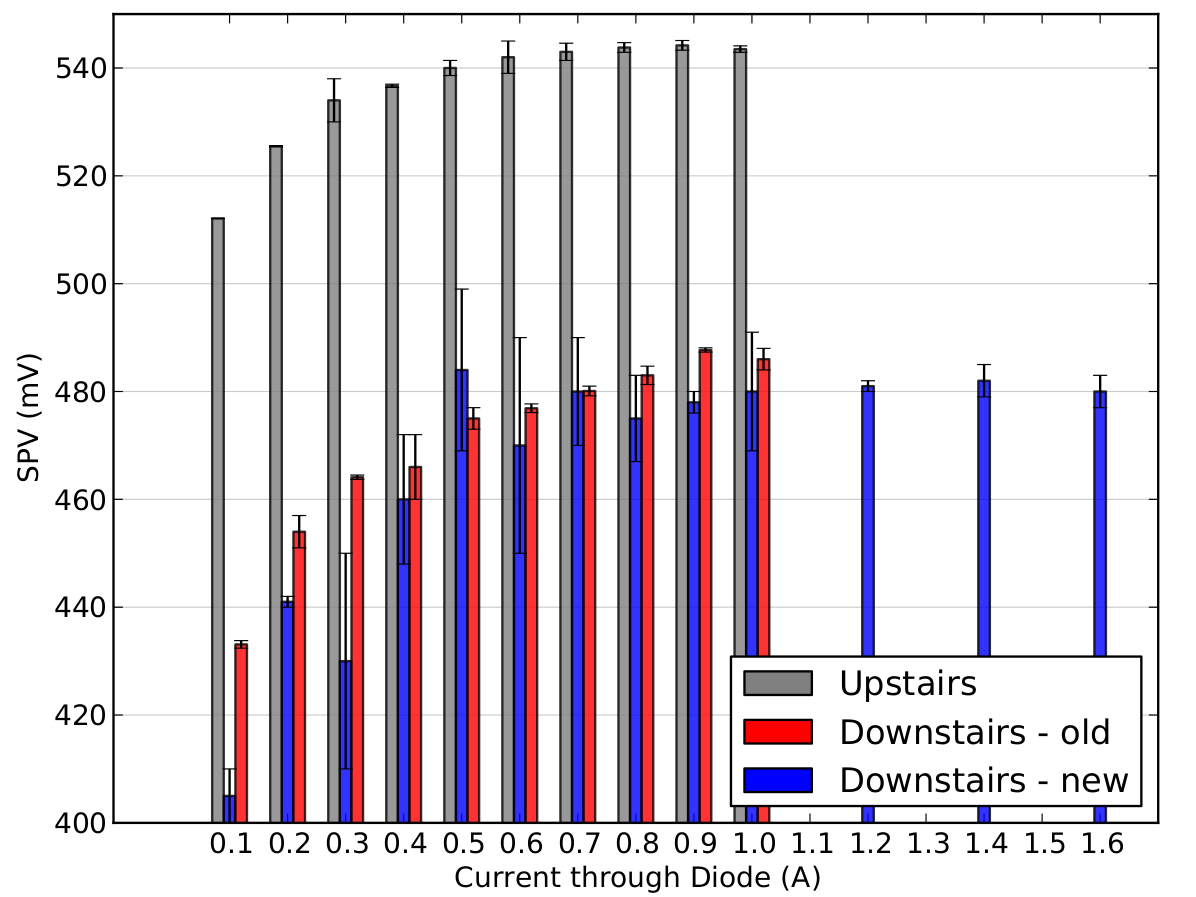
\includegraphics[width=0.8\linewidth]{./figs/currentseries}
	\caption{Comparison of the measured \spv{} as a function of illumination level as evidenced by the current through the \led{}. \enhyphen{Upstairs} refers to the combination of \led{} and the ambient probe station, while \enhyphen{Downstairs} refers to measurements with the \led{}, the \McA{} cryostation and the custom Lakeshore \kp{} probe head. \enhyphen{Old} signifies the weaker, damaged \led{} of nominally \SI{4200}{\lumen} intensity, while \enhyphen{new} refers to the fully functional \led{} of \SI{5400}{\lumen} intensity. Note that the measurement saturates independent of illumination intensity (\enhyphen{old} vs. \enhyphen{new}) at a lower measured \spv{} than the comparison with the ambient probe station.}
	\label{fig:Iseries}
\end{figure}
In that Figure \enhyphen{Upstairs} refers to the measurement in the ambient probe station, 'Downstairs' refers to the measurement with the \McA{} probe head, \enhyphen{old} refers to the initial \led{} with only 12 of 25 spots working and \enhyphen{new} refers to the newly purchased \led{} in which all diodes are working and which achieves a maximum illumination of \SI{5200}{\lumen}. It has to be pointed out that the new \led{} could be driven further than up to a maximum of \SI{1.0}{\ampere} to reach its full illumination intensity at a maximum current of \SI{1.6}{\ampere}, so the experiment was extended to make use of the maximum achievable intensity. As can be seen, saturation of the \spv{} is readily achieved with the \led{} in ambient at a current of \SI{0.6}{\ampere} and the measured value of \SI{540+-10}{\milli\volt} is in good agreement with the value expected from the measurement of the \spv{} with a xenon light source. It is furthermore apparent that the measurement achieves saturation. At a current of about \SI{0.8}{\ampere}, a further increase in current does not result in a corresponding significant increase in measured surface photovoltage. However, there is a significant discrepancy of \SI{60}{\milli\volt}~\footnote{about \SI{10}{\percent} of the maximum signal} in measured \spv{} between the two systems which cannot readily be explained. A similar experiment using neutral density filters to control the light intensity was carried out, but no meaningful conclusions could be drawn from the results, so it is not presented here. In a following step, the \spv{} of the alumina sample was measured with the Lakeshore not completely assembled. The vacuum chamber's lid as well as the radiations shielding chamber's lid were removed and the \led{} was held by hand as close to the probe head as possible without interfering with the measurement~\footnote{a constant stream of argon was employed to avoid undue contamination of the inner chamber from ambient.}. This configuration obviously does not represent a working condition for the Lakeshore, nor is it readily reproducible because of its vague parameters, but an \spv{} of $\sim$ \SI{480}{\milli\volt} could be achieved in this way. At this point, the nature of the \SI{60}{\milli\volt} discrepancy remains unknown. It might be due to the increased distance between the source and the sample or it might be due to partial absorption by the Lakeshore's windows, especially the \ir{}-shielding sapphire glass but the results obtained here remain hard to interpret properly. Saturation is achieved, but not at the right level. Simply using a stronger source will therefore most likely not alleviate the problem. It may be tried to replace the windows by lenses which better focus the light beam onto the sample but is is questionable if such a scheme is practically feasible or indeed even helpful. Practically, such window-lenses would have to be able to withstand \uhv{} conditions and saturation was achieved in ambient even without a lens, where the distance between sample and source is comparable to the corresponding distance in the cryogenic system. Since no explanations of the source of the discrepancy between the systems are forthcoming, a systematic experimental uncertainty of underestimating the \spv{} by about \SI{10}{\percent} has to be assumed when using the Lakeshore in conjunction with the \led{}.


\section{Temperature dependent measurement of the \spv{}}
Since it was established that temperature dependent \cpd{} measurements could reliably be carried out and that, albeit with a systematic uncertainty, \spv{} measurements could also be carried out with the Lakeshore cryogenic system, the final step was to attempt a combined experiment and carry out a temperature dependent measurement of the surface photovoltage. To this end, a suitable sample needed to be identified. This sample should have a sufficiently large photo-response and should undergo some phase transition at a well defined, critical temperature. Three different systems were investigated: biological samples consisting of a plant's photo-system immobilized on a gold surface; a lead-iodide-chloride perovskite on titanium-dioxide and finally a thin layer of vanadium oxide.\\
The biological samples exhibited changes in \cpd{} on the order of \SI{20}{\milli\volt}. These changes occurred at a well defined temperature, from \SIrange{250}{260}{\kelvin}. While interesting, these changes but were too small to serve as a reliable system for a proof of principle: \SI{20}{\milli\volt} is within the experimental uncertainty of both the \cpd{} and the \spv{} measurements. The biological samples were therefore quickly abandoned.\\
For the perovskites, it was attempted to compare their reaction when exposed to different parts of the optical spectrum, namely to compare their dark \cpd{} to the \cpd{} when exposed to full spectrum illumination and when exclusively exposed to infra-red illumination. The perovskite sample was introduced to the inner chamber of the Lakeshore and electrically contacted with the help of a conductive clip and screw. To allow for electrical connection via the back contact, the perovskite was removed from the point where the clip contacted the sample. The cryogenic system was evacuated and seven temperatures where chosen at which to measure the \cpd{}: \SIlist{130;170;210;230;250;270;280}{\kelvin}. At each of these temperatures, the dark \cpd{} was measured. A filter which would only allow \ir{} radiation to pass was placed in front of the source, the sample was briefly illuminated and the \ir{} \cpd{} was measured. The \cpd{} of the system was allowed to decay back to its original dark value and the filter was removed. The system was then briefly illuminated by full spectrum at high intensity and the light \cpd{} was measured. The \cpd{} of the system was allowed to decay back to its original dark-value and the system was then cooled down to the next temperature step. In the course of this measurement, repositioning the probe head to new positions over the sample was necessary because although care was taken, crashing the probe head onto the sample could not be avoided. The whole experiment was carried out under low pressure conditions, but for the lowest five temperature points, the pressure was about a factor ten lower than for the measurements taken at \SIlist{270;280}{\kelvin}. To carry out the experiment, the set up of the \McA{} had to be modified twofold. Measurements had to be carried out without the inner chamber's sapphire glass window as this would exclude any infra-red radiation from reaching the samples in the first place. Secondly, the xenon lamp had to be used as a source of illumination to give access to the infra-red part of the spectrum. These modifications introduced experimental difficulties for several reasons. As already pointed out, the xenon lamp is a source of heat and therefore, an unknown experimental uncertainty in the temperature was introduced. The experiment had to be carried out very quickly to avoid damage to the system and to minimize said uncertainty in temperature. In effect, only a brief flash of illumination could be allowed to reach the sample. Furthermore, the xenon lamp and its high power electrical source had to be set up in close proximity to the Lakeshore cryogenic system and electrical noise due to the relatively high currents and voltages involved in this experiment were introduced. To add to these problems, the sample was neither fresh nor necessarily stable and perovskites are inherently complicated systems. Accordingly, the results did not show a clear variation with temperature and could not be reproduced on consecutive days. Therefore, it was decided that this experiment could not serve for the purpose of showing a reliable \spv{}(T) measurement.\\

\subsection{Vanadium oxide}
\label{sec:vox}
\subsubsection{Description of samples and preliminary research carried out at the Cahen group}
Vanadium-dioxide (\vadiox{}) is a system well known for undergoing a metal to insulator transition (\mit{}) close to room temperature. At the heart of this transition lies a reconfiguration of the of the crystal lattice, where \vadiox{} transitions from its high-temperature tetragonal (rutile) phase to a low temperature monoclinic phase. In the tetragonal phase, the Fermi level of the material is well within the conduction band and hence, the material behaves like a metal. In the monoclinic phase, an energy gap has developed and the material now behaves like an insulator~\cite{nakano_gapopen}. Of course, the only difference between an insulator and a semiconductor is the size of their energy gaps and if the transition occurs gradually, one might also speak of a metal-semiconductor-insulator transition instead of an \mit{}. This transitions has extensively been studied, using many different methods such as direct photoemission \& x-ray absorption spectroscopy~\cite{koethe_expstud}, Raman spectroscopy~\cite{radue_raman}, ultra-fast pump-probe spectroscopy~\cite{jensen_expgap} etc. However, because of their relative simplicity, studies of the resistivity of the material stick out~\cite{shibuya_physlet}. In these, changes of resistivity over several orders of magnitude are not uncommon. Finally, the \mit{} in \vadiox{} was also investigated using Scanning Kelvin Probe Microscopy, where $\sim$ \SI{200}{\nano\metre} thin stripes of the material were grown adjacent to a strip of gold. These strips were continuously scanned over a temperature range including the phase transition temperature ($T_{MI}$) of \vadiox{}. Gold provided a stable reference work function and thus, the work function of \vadiox{} could be measured in absolute terms. It was found that vanadium-dioxide has a work function of $\sim$ \SI{5.15}{\electronvolt} in its metallic phase and that the work function gradually decreased by $\sim$ \SI{0.15}{\electronvolt} over a range of \SI{60}{\kelvin}~\cite{ko_kp}. In other studies~\cite{shibuya_physrev}, it was found that \mit{} could be tuned by tungsten-doping of a thin film of \vadiox{} grown on a supporting matrix of \tiox{} and preliminary research into similar samples has already been carried out in the Cahen group.\\
The samples were either pure or \SI{2}{\percent} tungsten-doped vanadium-dioxide of thickness ranging from \SIrange{10}{80}{\nano\metre} grown on either \tiox{} or on niobium-doped titanium-dioxide (Nb:\tiox{}) and were kindly provided by M. Nakano of RKIEN. A change in resistivity of several orders of magnitude upon \mit{} could be shown for these samples. When used for this project, however, the collection of vanadium-dioxide samples had already been in storage inside a desiccator for more than a year. Many samples were damaged and proper storage throughout the year could not be guaranteed. Therefore, the choice of sample for this project was limited to pieces which, upon optical inspection, were closest to their initial appearance and were still large enough to allow proper positioning of the probe head over a sufficiently homogeneous surface. Therefore, a sample of \SI{50}{\nano\metre} \SI{2}{\percent} \wvadiox{} on pure \tiox{} was chosen. It had been investigated by Nir Kedem using the van der Pauw method with a temperature resolution $<$\SI{5}{\kelvin}. It showed an approximately two orders of magnitude change in resistivity with a relatively gradual profile, occurring over the temperature range from \SIrange{220}{270}{\kelvin}. The resistivity also exhibited hysteresis, with up to half an order of magnitude difference in resistivity between cooling down and heating up.
\subsubsection{Experimental procedure, results and discussion}
Initially, the work function of the vanadium-dioxide sample was determined with the ambient probe station. The sample was sonicated for three minutes each in acetone, ethanol and THF and was then blow-dried under \nitro{}. To calibrate the probe head, a fresh surface of \hopg{} was prepared and the \cpd{} was measured. The work function of the probe head was found to be \SI{5.085+-0.015}{\electronvolt}. The work function of the clean \wvadiox{} sample was determined to be \SI{5.17+-0.02}{\electronvolt}, in remarkable agreement with the value obtained by Ko \emph{et~al.}~\cite{ko_kp}.\\
Before each measurement, the sample was subjected to the same cleaning procedure outlined above. The sample was then blow-dried under \nitro{} and placed directly on the ground of the inner chamber of the Lakeshore. Electrical contact was made from the top using a conductive screw and clip. The Lakeshore was then evacuated and the experiment commenced once a stable vacuum condition was obtained.\\
In the first experiment, the Lakeshore was cooled down to the lowest temperature achievable by liquid nitrogen cooling: \SI{97}{\kelvin} for this cryogenic system. During this cool-down, the \cpd{} was quickly measured at three points where the temperature remained relatively stable for a sufficient time. Once the lowest possible temperature was reached, the flow of nitrogen was stopped, the heater was set to \SI{300}{\kelvin} and the \cpd{} was measured continuously. This protocol allows for a quick measurement of the \cpd{}(T)-response of the system to identify the temperature range of interest, but uncertainties in temperature are introduced because of the temperature gradient present in the inner chamber and because of having to note down the temperature manually. The experiment had to be aborted. The data obtained during this initial experiment are shown in Figure \ref{fig:vox1}.\\
\begin{figure}
\centering
	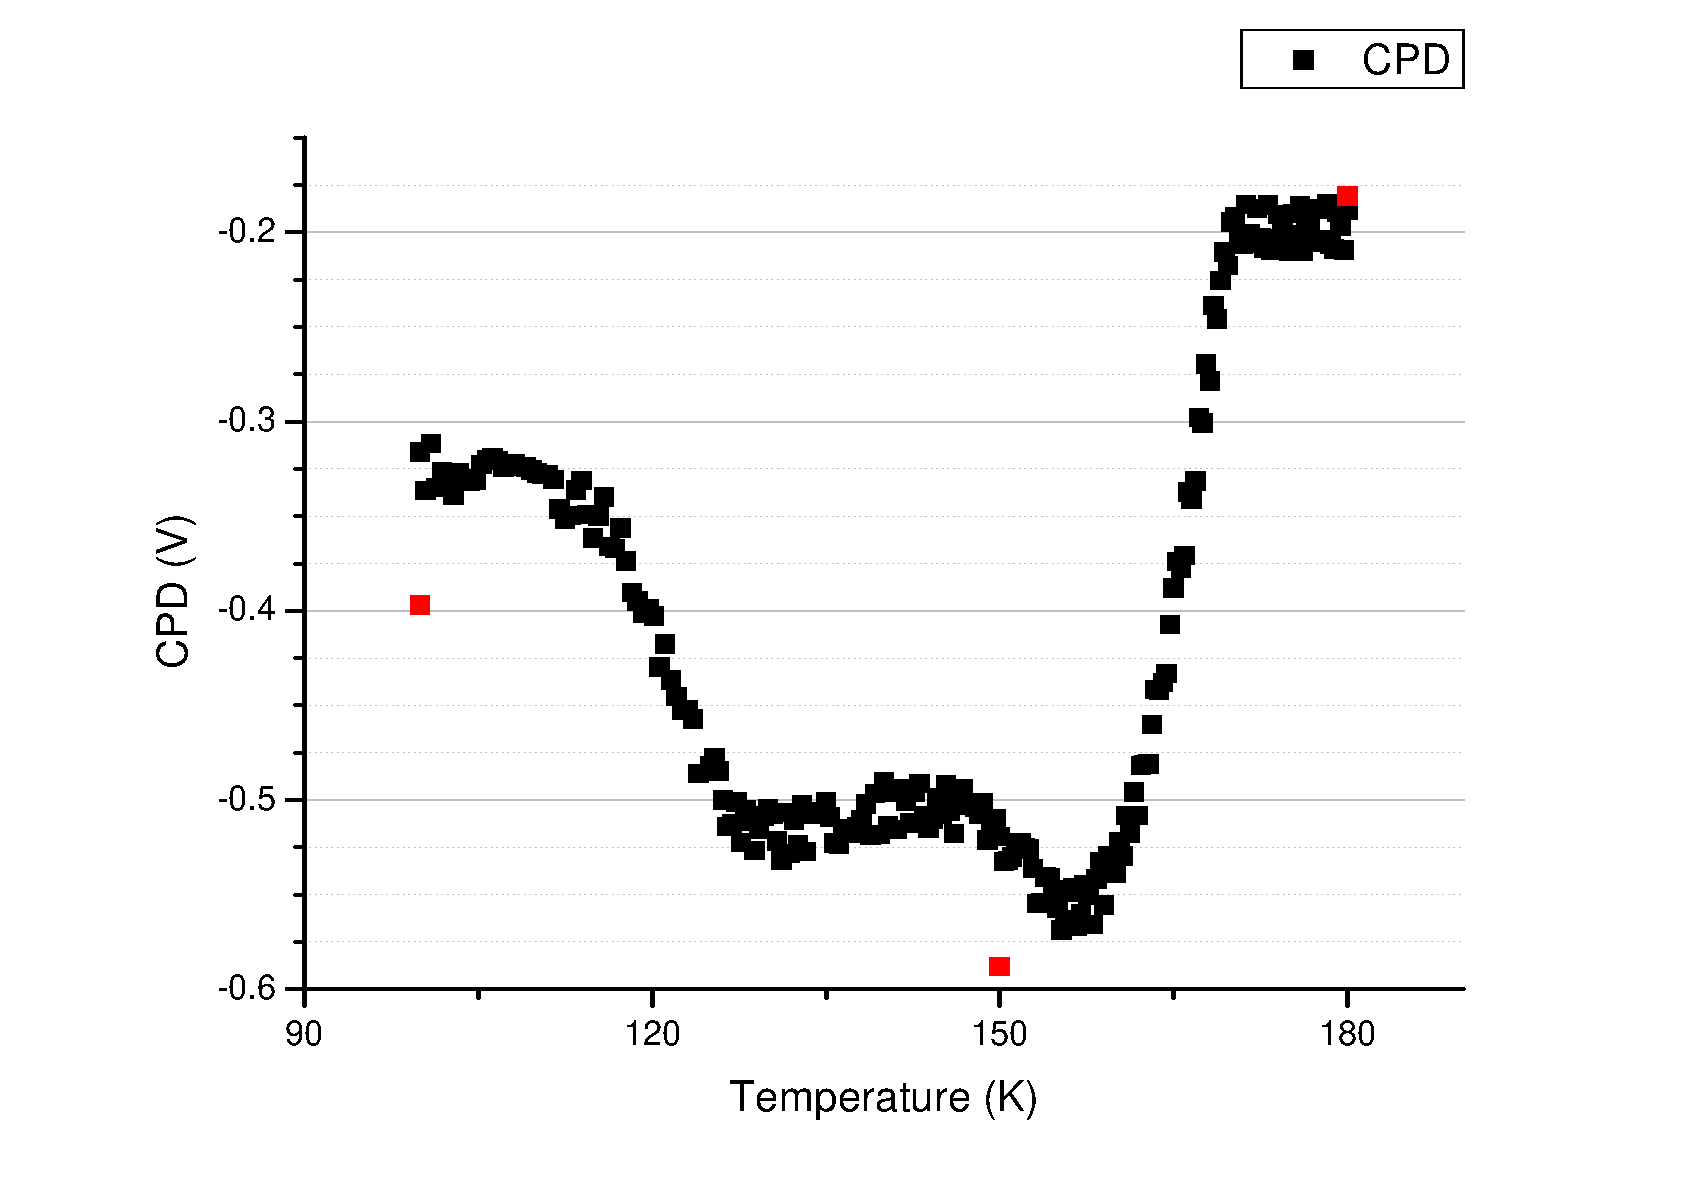
\includegraphics[width=0.8\linewidth]{./figs/vox1}
	\caption{Raw data of the contact potential difference of the \wvadiox{} sample obtained during a temperature-sweep. Data points in red were obtained while cooling down, data points in black were recorded while warming up.}
	\label{fig:vox1}
\end{figure}
For the next experiment, the temperature range was extended and more care was taken to more accurately determine the temperature. The system was cooled down to \SI{100}{\kelvin} and gradually increased. The \cpd{} was measured at 11 well defined temperatures. For each of these temperatures, the flow of liquid nitrogen and the heater setting were carefully adjusted until all three of the cryogenic system's temperature read-outs were within a range of \SI{5}{\kelvin} of each other. Holding the temperature constant, the \cpd{} was then recorded once every second for a period of 100 seconds and these data were averaged. The temperature was increased to the next set-point and the procedure was repeated. The observations of this experiment are plotted in Figure \ref{fig:vox2}. The uncertainty in \cpd{} was taken to be twice the standard deviation of \cpd{} values obtained during the 100 second period. Uncertainty in temperature is not shown but assumed to be less than \SI{5}{\kelvin}.\\
\begin{figure}
\centering
	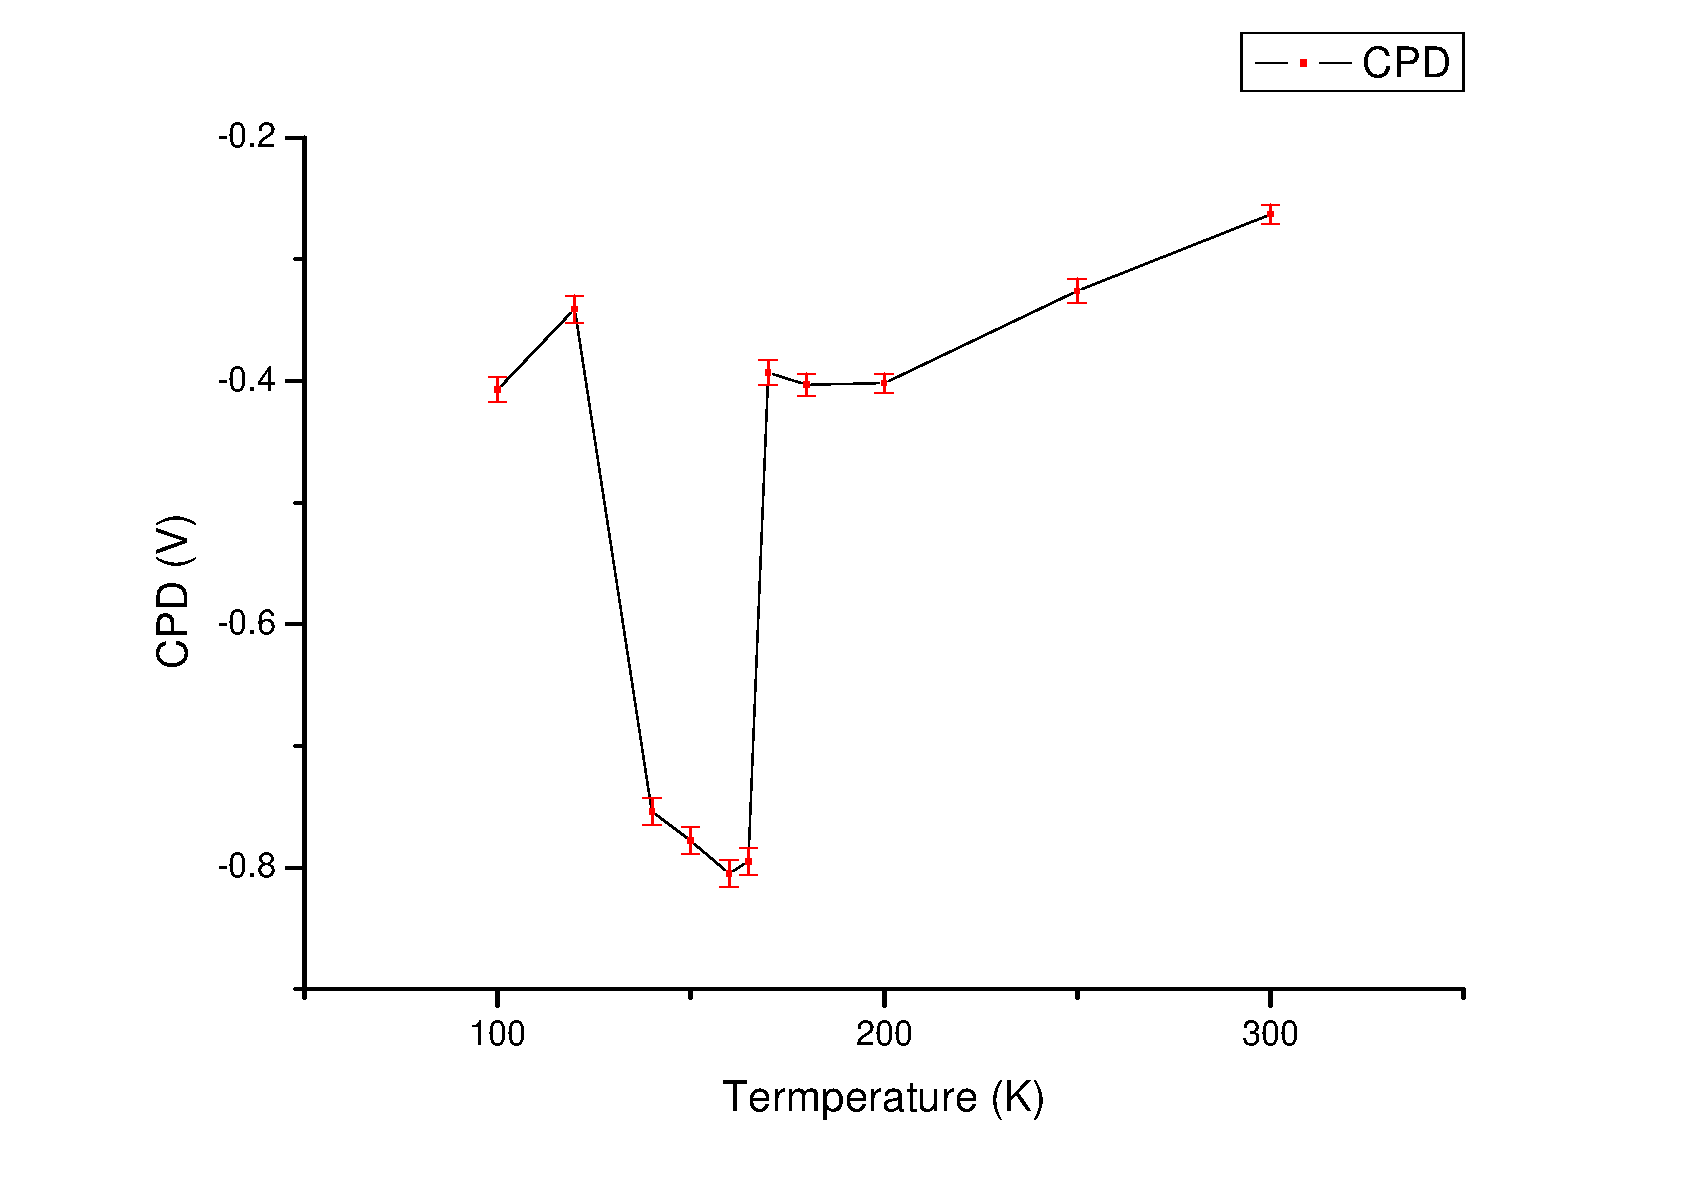
\includegraphics[width=0.8\linewidth]{./figs/vox2}
	\caption{The contact potential difference of the \wvadiox{} sample as a function of temperature. Experimental uncertainties are explained in the text.}
	\label{fig:vox2}
\end{figure}
In the last experiment, both dark and light \cpd{} were measured for the same sample for a range of temperatures between 180 and \SI{300}{\kelvin} in intervals of \SI{20}{\kelvin}. \cpd{} was only measured once the temperature gradient inside the Lakeshore was less than \SI{5}{\kelvin}. For each temperature, dark \cpd{} was measured once every second over a period of 100 seconds and these data were averaged. Illumination for light \cpd{} was achieved by the \led{} at maximum intensity and to avoid possibly heating the sample, light \cpd{} was measured for 15 seconds. \hopg{} as a reference for the work function was not used in this experiment. Instead, the work function of the sample at \SI{300}{\kelvin} in vacuum was assumed to be the same as that obtained from the same sample at room temperature in ambient and the work function of the probe could therefore be calculated to be \SI{4.41}{\electronvolt}. The results of this final experiment are shown in Figure \ref{fig:vox3}. The experimental uncertainty in work function includes twice the standard deviation of dark \cpd{} obtained during the 100 second interval plus an added uncertainty from the calculation of the work function of the probe head. The experimental uncertainty in \spv{} includes uncertainty from dark \cpd{} as well as that for light \cpd{}. Uncertainty in temperature is, again, not shown, but assumed less than \SI{5}{\kelvin}.\\
Probably the most remarkable feature of these measurements is the sudden drop in \cpd{} (sudden rise in \wf{}) at $\sim$ \SI{120}{\kelvin} and the consequent sudden rise in \cpd{} around $\sim$ \SI{170}{\kelvin} seen in both Figure \ref{fig:vox1} and Figure \ref{fig:vox2}. Since these features were observed during cool down as well as during heating up in the first and were again observed in the second, independent measurement, they are most likely not an artefact of the measurement, nor should they be ascribed to simple experimental failure. They represent a change in work function of $\sim$ \SIrange{200}{400}{\milli\electronvolt} which is remarkably large. Such changes can most likely not be explained by changes in shielding of accumulated surface-charges or repositioning of the Fermi level. A (reversible) surface-reconstruction or even a (reversible) change of chemical composition might be able to explain the data, but without further measurements, we cannot be sure. To the best of my knowledge, neither a structural reconstruction nor a change in \wf{} at the temperatures is question has yet been reported in the literature for \wvadiox{}. In conjunction with the measurements carried out by Nir Kedem, the experiments reported in the literature and those summarised in Figure \ref{fig:vox3}, it has to be assumed that the changes in \wf{} seen at around \SIlist{120;170}{\kelvin} are not explained by the known \mit{} of vanadium-dioxide. The difference in \cpd{} between heating up and cooling down seen in Figure \ref{fig:vox1} might be taken as evidence for hysteresis at lower temperatures than previously observed, but the data is sparse, so no conclusive explanation can be drawn from them. Figure \ref{fig:vox2} on the whole corroborates what was observed in the initial, relatively inaccurate experiment even though the size of the observed effect is greater, but nothing more can be concluded from these measurements alone.\\
\begin{figure}
\centering
	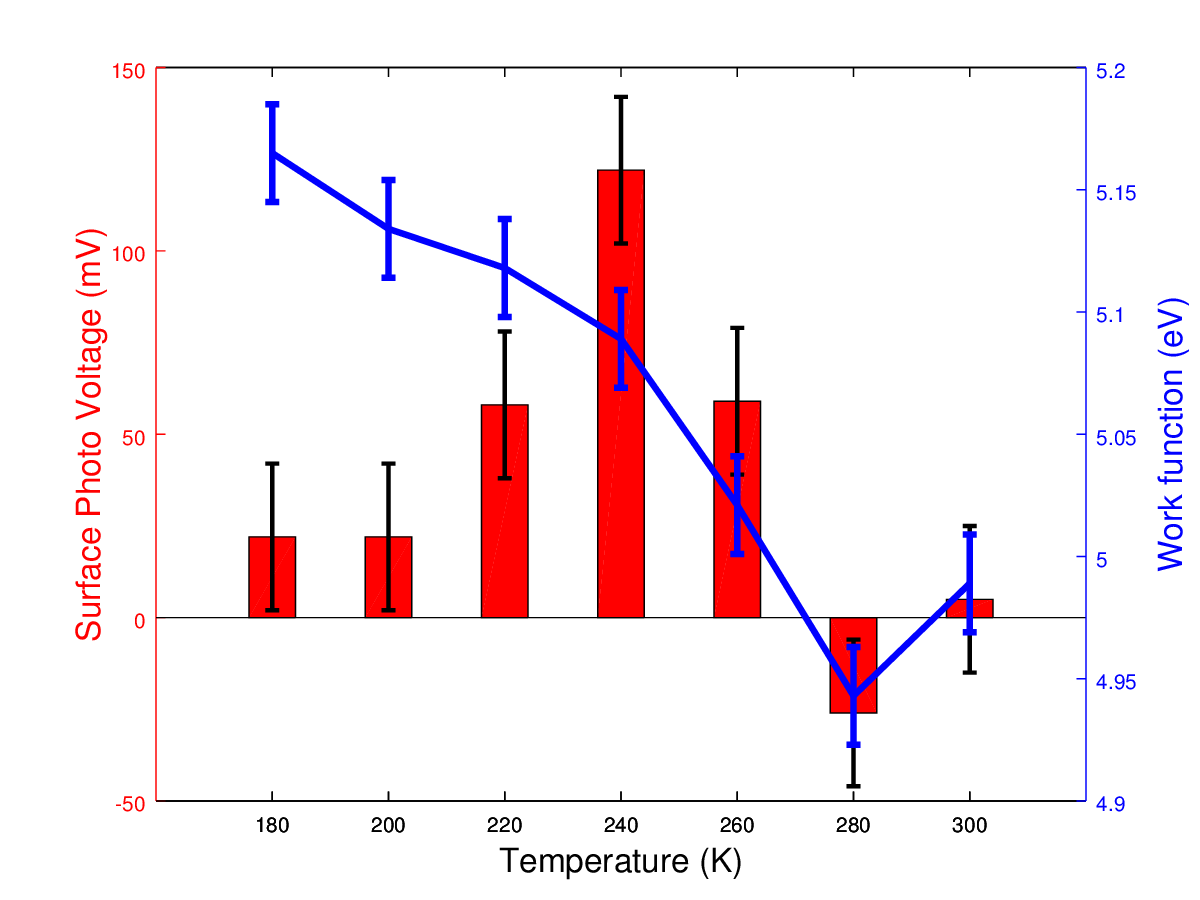
\includegraphics[width=0.8\linewidth]{./figs/vox3}
	\caption{Measured surface photovoltage and calculated work function for the \wvadiox{} sample as a function of temperature. The appearance of an \spv{} coincides with the \mit{} temperatures observed in earlier measurements, its positive sign indicates an n-type semiconductor. The change in \wf{} is substantial but remains unexplained without further experiments. Experimental uncertainties are explained in the text.}
	\label{fig:vox3}
\end{figure}
We will now concentrate on the measurement of the \spv{} as shown in Figure \ref{fig:vox3}. A significant \spv{} is observed below \SI{280}{\kelvin}, at \SI{240}{\kelvin} the \spv{} is at its maximum of $\sim$ \SI{120}{\milli\volt} and below \SI{220}{\kelvin} \spv{} is reduced back to levels comparable to those at room temperature. A significant \spv{} signal is therefore observed in the same temperature range that was identified for \mit{} in the resistivity measurements. In the metallic rutile configuration, no \spv{} is observed and none is expected. As the energy gap of the material gradually widens, the \spv{} gradually increases because gradually less thermally free carriers can shield trapped surface charges in the dark condition. The simultaneous presence of both phases of vanadium-dioxide over a range of temperatures has been observed in the literature~\cite{pergament_mixphase}. As a result, band bending and hence observed \spv{} gradually increase. If the \spv{} is assumed to be saturated at \SI{240}{\kelvin} and, accordingly, the bands to be flattened, the band bending is $\sim$ \SI{120}{\milli\electronvolt}. Possible Fermi level pinning would add to the size of the band bending, so the stated value has to be seen as a minimum. On first sight, the gradual decrease in \spv{} signal might be puzzling. One would expect the trend for the \spv{} to continue, after all, the idea behind low temperature \spv{} is to counteract thermally free carriers and increase the influence of electron-hole pairs created by absorption of light. However, the observation made here can be explained if one recalls that vanadium-dioxide is undergoing a metal to \emph{insulator} transition and that for an insulator, the energy gap is expected to be relatively large. Looking at the spectrum of illumination, Figure \ref{fig:ledspec}, a clear cut off below \SI{400}{\nano\metre} is seen. \SI{400}{\nano\metre} radiation corresponds to a photon energy of $\sim$ \SI{3.1}{\electronvolt} so if the energy gap in \vadiox{} becomes larger than this, no carriers can be created by illumination or rather: only a minute fraction of incident photons corresponding to the minute fraction of photons at the low-wavelength tail of the \led{} will have sufficient energy to create free carriers. Therefore, the sample is no longer saturated by illumination and a significant drop in observed \spv{} signal is expected. A problem with that interpretation is that the band gap of vanadium-dioxide is consistently reported as $\sim$ \SI{0.7}{\electronvolt}, from theoretical~\cite{biermann_theogap} as well as from experimental studies~\cite{garcia_expgap,jensen_expgap,koethe_expstud,merenda_expgap}.\\
Concentrating on the temperature range 180 to 300 K, a change in \wf{} of $\sim$ \SI{150}{\milli\electronvolt} is seen in both in Figure \ref{fig:vox2} and, more clearly, in Figure \ref{fig:vox3}. So far, positive changes of \wf{} of up to \SI{450}{\milli\electronvolt} have been observed for bundlelike \vadiox{} nanostructures~\cite{yin_450change}. A change of $\sim$ \SI{150}{\milli\electronvolt} was also reported by Ko~\cite{ko_kp} during the \mit{} of vanadium-dioxide, but they observed a decrease instead of the increase in \wf{} seen here. The difference between the sample used in their research and the one used here is the presence of tungsten as dopant. Tungsten has more valence electrons than vanadium even in its elemental state and certainly has more valence electrons than vanadium in its oxide. Tungsten should therefore act as n-type dopant. This is in accordance with the sign of \spv{} observed in Figure \ref{fig:vox3}. The change in \wf{} can not be explained by a gradual change in the position of the Fermi level: for an n-type material, $E_f$ is expected to increase with lowering temperature. The carrier concentrations inside the material might change drastically due to dopant freeze-out or other mechanism and that might change $E_f$ sufficiently to account for the rise in \wf{}, but without further experiments, these attempted explanations remain speculative. In fact, there is doubt in the literature if a simple `gap opening process' can indeed explain the observed \mit{}~\cite{eyert_theobands,booth_theobands}. Judging by the complexity of the material, attempts at explaining the observed data in terms of simple band diagram considerations of typical metals and n-type semiconductors will fall short. Similar experiments with an extended spectral range or a more detailed study of spectral surface photovoltage might serve to verify the results obtained for this material here, but they are out of scope of this project: elucidating the finer details of the \mit{} observed in \wvadiox{} was not the aim of this project. Vanadium-dioxide was, above all, chosen as a system to show a viable \spv{}(T) measurement, to serve as a proof of concept for measuring temperature dependent \spv{} with the Lakeshore cryogenic system. This was achieved with these experiments.

\section{Conclusion}
A series of experiments showed the viability of using the Lakeshore cryogenic system equipped with a \McA{} Kelvin probe head and an \led{} illumination source as a system to measure temperature dependent changes in the surface photovoltage. To do so, the \cpd{} obtained under various circumstances, namely in ambient, under low pressure and at temperatures below freezing was compared to existing, trusted systems. Deviations between the systems were within normal, acceptable experimental uncertainties usually encountered when using Kelvin Probe measurements. The \spv{} obtained from measurements in the Lakeshore at room temperature was shown to agree with \spv{} measurements carried out in the ambient system and lastly, experiments to show a viable \spv{}(T) measurement were carried out. Some aspects of these experiments were shown to be in good agreement with earlier, preliminary research carried out in the Cahen group and with results reported in the literature while the finer detail and precise interpretation of all the observed features remains elusive without further investigations. However, with vanadium-dioxide, it could be shown that interesting and reproducible data can be obtained by using the Lakeshore cryogenic system for \cpd{}(T) and \spv{}(T) measurements.




\appendix
	\label{chap:app}
	\bibliographystyle{timounsrt}
	\bibliography{biblio}
%	\include{./tex/Appendix}
	
\end{document}
